% Created 2023-10-29 Sun 06:42
% Intended LaTeX compiler: pdflatex
\documentclass[11pt,oneside]{memoir}
\makeatletter

\usepackage{answerkey-env}

\ifanswerkey
  \usepackage[forcolorpaper, answerkey]{eqexam}
  \usepackage{vinaya-class-questions}
\else
  \usepackage[forcolorpaper, nosolutions]{eqexam}
  \usepackage[nosolutions]{vinaya-class-questions}
\fi

\proofingsymbolColor{linkred}
\fillinColor{linkred}

\def\maketitle{}

\maxtocdepth{subsection}

\newenvironment{twocols}{%
  \raggedright%
  \setlength{\parindent}{0pt}%
  \setlength{\parskip}{8pt}%
  \fontsize{11}{17}\selectfont%
  \begin{multicols}{2}%
}{%
  \end{multicols}%
}

\newenvironment{widecols}{%
  \hspace*{-0.05\linewidth}\begin{minipage}{1.1\linewidth}%
  \raggedright%
  \setlength{\parindent}{0pt}%
  \setlength{\parskip}{8pt}%
  \fontsize{11}{17}\selectfont%
  \begin{multicols}{2}%
}{%
  \end{multicols}%
  \end{minipage}%
}

\newlength\@tmp@width
\newlength\@tmp@height

\renewcommand*{\printchaptertitleHook}{%
  \AddToShipoutPictureBG*{%
    \put(\LenToUnit{\paperwidth-25mm-\spinemargin},\LenToUnit{\paperheight-95mm}){%
      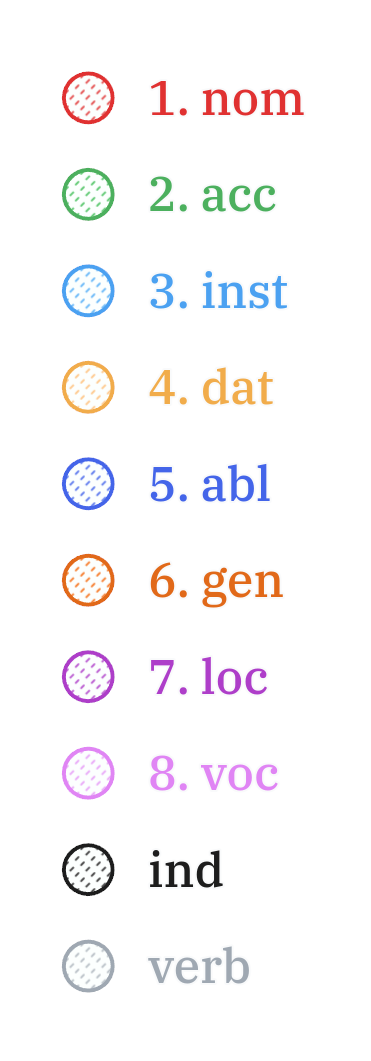
\includegraphics[width=25mm]{./images/cases-legend-white-large.png}%
    }%
  }%
}

\newcommand*\sentenceDiaMsg{\textbf{Exercise:} Draw a sentence analysis diagram below and indicate declensions.}

\newcommand*\sentenceDiaSolution[2][0.4]{%
  \ifanswerkey%
    \hspace*{-\spinemargin}%
    \begin{minipage}{\paperwidth}%
      \centering%
      \includegraphics[scale=#1]{#2}%
    \end{minipage}%
  \else%
    \settototalheight{\@tmp@height}{\includegraphics[scale=#1]{#2}}%
    \begin{minipage}[\@tmp@height]{\linewidth}%
      \sentenceDiaMsg%
    \end{minipage}%
  \fi%
}

\usepackage{cwpuzzle}

\renewcommand\PuzzleCluePre{%
  \begin{minipage}[t]{0.75\linewidth}%
}

\renewcommand\PuzzleClueFont{\fontsize{11}{17}\selectfont}

% \def\PuzzleThickline{\linethickness{2pt}}

\makeatother

\date{\today}
\title{Pali Lessons}
\hypersetup{
 pdfauthor={The Bhikkhu Saṅgha},
 pdftitle={Pali Lessons},
 pdfkeywords={},
 pdfsubject={},
 pdfcreator={Emacs 29.1 (Org mode 9.6.6)}, 
 pdflang={En_Gb}}
\begin{document}

\maketitle
\frontmatter

{\centering

{\Huge Pāḷi Lessons}

\bigskip
\href{https://vinaya-class.github.io}{https://vinaya-class.github.io}

{\scshape\small last updated on}\\
\today

}

\newlength{\colOne}\setlength{\colOne}{0.35\linewidth}
\newlength{\colTwo}\setlength{\colTwo}{0.6\linewidth}

\bigskip
\tableofcontents*

\mainmatter

\chapter{Lesson 1}
\label{sec:org5ce0fa5}
\section{Language Notes}
\label{sec:orgbe11786}

The \textbf{gender of a noun} is either masculine, feminine or neuter.
Its \textbf{number} is either singular or plural.
Its \textbf{declension} have eight cases, which indicate the subject, object, location, etc.

\textbf{Nouns ending} in \emph{-a} are either masculine or neuter. Nouns ending in \emph{-ā} are feminine.\\[0pt]
Other nouns end in \emph{-i, -ī, -u, -ū}.

\textbf{Word order} in the simplest case is Subject-Object-Verb, but since the case indicates the role of a noun, word order is often altered for emphasis.

\begin{center}
\begin{tabular}{ll}
Sūdo \emph{(nom.sg.)} bhattaṁ \emph{(acc.)} pacati \emph{(3rd.sg.)}. & Dārakā \emph{(nom.pl.)} bhojanīyaṁ \emph{(acc.)} bhuñjanti \emph{(3rd.pl.)}.\\[0pt]
The chef cooks the rice. & The boys eat the food.\\[0pt]
\end{tabular}
\end{center}

The \textbf{subject} and \textbf{verb} must agree in number: \emph{Sakuṇā ākāse uḍḍayanti} (Birds fly in the sky).

\begin{center}
\begin{tabular}{lll}
Sakuṇ\textbf{ā} & masc.nom.\textbf{pl.} & Birds\\[0pt]
ākāse / ākāsamhi / ākāsasmiṁ & masc.loc.sg. & in the sky\\[0pt]
uḍḍaya\textbf{nti}. & pr.3.\textbf{pl.} & they fly.\\[0pt]
\end{tabular}
\end{center}

The verb `to be' (is / are) is often implied and dropped from the sentence.

\textbf{An adjective} agrees with the noun it qualifies in gender, number and case. \\[0pt]
Generally, the order is adjective + noun. E.g. \emph{seto asso:} a white horse, \emph{setā assā:} white horses.

\textbf{Adverbs} are indeclinable: \emph{idha} (here), \emph{tattha / tatra} (there), \emph{tato}
(from there), \emph{idāni} (now), \emph{pubbe} (before), \emph{pacchā} (after), etc.

\bigskip

\begin{multicols}{2}

\textbf{Plural / singular} for nominative cases:

\begin{center}
\begin{tabular}{lll}
masc.sg. & -o & devo\\[0pt]
masc.pl. & -ā & devā\\[0pt]
\hline
nt.sg. & -aṁ & rūpaṁ\\[0pt]
nt.pl. & -ā, -āni & rūpāni\\[0pt]
\hline
fem.sg. & -ā & vedanā\\[0pt]
fem.pl. & -ā, -āyo, & vedanāyo\\[0pt]
\end{tabular}
\end{center}

\columnbreak

Personal pronouns in nominative case:

\begin{center}
\begin{tabular}{lll}
 & \textbf{sg.} & \textbf{pl.}\\[0pt]
\textbf{1st} & ahaṁ & amhe, mayaṁ, no\\[0pt]
\textbf{2nd} & tuvaṁ, tvaṁ & tumhe, vo\\[0pt]
\textbf{3rd.masc.} & so, sa & te\\[0pt]
\textbf{3rd.nt.} & taṁ, tad & tāni\\[0pt]
\textbf{3rd.fem.} & sā & tā, tāyo\\[0pt]
\end{tabular}
\end{center}

\emph{sā taṃ bhāsati:} she speaks (to) him/them

\vspace*{-\baselineskip}

\begin{center}
\begin{tabular}{lll}
ta → & \emph{(nom.sg.)} so / taṁ / sā & \emph{(nom.pl.)} te / tāni / tā, tāyo\\[0pt]
 & \emph{(acc.sg.)} taṁ & \emph{(acc.pl.)}  te / tāni / tā, tāyo\\[0pt]
\end{tabular}
\end{center}

\end{multicols}
\bigskip

The 1st and 2nd personal pronouns are gender neutral, the 3rd person pronouns are gendered.

Pronouns take on the person and number of the noun they represent.

\clearpage

A relative sentence begins with a relative clause, followed by a demonstrative:

\begin{center}
\begin{tabular}{lll}
\emph{yo} & \emph{gilānaṃ} & \emph{upaṭṭhāti}\\[0pt]
he who & to the ill & attends\\[0pt]
\emph{so} & \emph{maṃ} & \emph{upaṭṭhāti}\\[0pt]
he & to me & attends\\[0pt]
\end{tabular}
\end{center}

\bigskip

\begin{multicols}{2}

\textbf{Negation:} The particle \emph{na} before verbs, shortened as the \emph{a-} prefix for
nouns. \emph{mā + aorist past} is a (present) prohibition.

\emph{avera:} [na + vera] non-hostility \\[0pt]
\emph{Na jānāmi.} I don't know. \\[0pt]
\emph{Mā akāsi!} Don't you do!

\columnbreak

\textbf{Questions} begin with interrogatives such as \emph{api, api nu, kiṁ, kahaṁ, kathaṁ}.
\emph{Kiṁ} may be placed at the end of the sentence.

\emph{Api nu gacchasi?} Do you go?\\[0pt]
\emph{Kiṁ nāmo si?} What is your name?\\[0pt]
\emph{Gacchasi kiṁ?} Do you go?

\end{multicols}

\textbf{Declension Table: Masculine Nouns Ending in -a}

\begin{center}
\begin{tabular}{llll}
Case & Singular & Plural & Meaning (sg.)\\[0pt]
\hline
1. Nominative & nar\textbf{o} & nar\textbf{ā} & the man does sth (object)\\[0pt]
2. Accusative & nar\textbf{aṁ} & nar\textbf{e} & sth happens to the man (subject)\\[0pt]
3. Instrumental & nar\textbf{ena} & nar\textbf{ehi} & by, with, through the man\\[0pt]
4. Dative & nar\textbf{āya}, nar\textbf{assa} & nar\textbf{ānaṁ} & to the man, for the man\\[0pt]
5. Ablative & nar\textbf{ā}, nar\textbf{amhā}, nar\textbf{asmā} & nar\textbf{ehi} & from the man\\[0pt]
6. Genitive & nar\textbf{assa} & nar\textbf{ānaṁ} & of the man, the man's\\[0pt]
7. Locative & nar\textbf{e}, nar\textbf{amhi}, nar\textbf{asmiṁ} & nar\textbf{esu} & in, on, at the man\\[0pt]
8. Vocative & nar\textbf{a}, nar\textbf{ā} & nar\textbf{ā} & Hey, man!\\[0pt]
\end{tabular}
\end{center}

This the most common declension, worth memorizing by heart. 87\% of all masculine
nouns are ending in \textbf{-a}, \mbox{97\% of} all neuter nouns are ending in \textbf{-aṁ}, in
addition to adjectives and participles with the same declensions.

\section{Simple Present Tense (-āmi, -asi, -ati)}
\label{sec:org7d0a4b8}

Actions that are happening at the present moment, occurring regularly, or general truths.

Verbal bases can end in \emph{-a, -ā, -e, -o}.

\bigskip
{\centering\par
\begin{multicols}{2}

Verbal terminations:

\begin{center}
\begin{tabular}{lll}
 & \textbf{sg.} & \textbf{pl.}\\[0pt]
\textbf{1st} & -mi & -ma\\[0pt]
\textbf{2nd} & -si & -tha\\[0pt]
\textbf{3rd} & -ti & -(a)nti\\[0pt]
\end{tabular}
\end{center}

The base is obtained by removing the 3rd.sg. termination \emph{-ti} from the conjugated form.

\columnbreak

Root: \emph{√dhāv} (to run), base: \emph{dhāva}

\begin{center}
\begin{tabular}{lll}
 & \textbf{sg.} & \textbf{pl.}\\[0pt]
\textbf{1st} & dhāvāmi & dhāvāma\\[0pt]
\textbf{2nd} & dhāvasi & dhāvatha\\[0pt]
\textbf{3rd} & dhāvati & dhāvanti\\[0pt]
\end{tabular}
\end{center}

The final \emph{-a} of the base is lengthened before \emph{m}: \emph{dhāvāmi, dhāvāma}.

\end{multicols}
\par}
\bigskip
\begin{multicols}{2}
\setlength{\columnseprule}{0pt}

\begin{center}
\begin{tabular}{ll}
he goes & gacchati\\[0pt]
we go & \fillin{4cm}{gacchāma}\\[0pt]
he comes & āgacchati\\[0pt]
they come & \fillin{4cm}{āgacchanti}\\[0pt]
he walks & carati\\[0pt]
they walk & \fillin{4cm}{caranti}\\[0pt]
he chews & khādati\\[0pt]
you (sg.) chew & \fillin{4cm}{khādasi}\\[0pt]
he eats (enjoys) & bhuñjati\\[0pt]
they eat & \fillin{4cm}{bhuñjanti}\\[0pt]
\end{tabular}
\end{center}

\columnbreak

\begin{center}
\begin{tabular}{ll}
he sees & passati\\[0pt]
you (sg.) see & \fillin{4cm}{passasi}\\[0pt]
he recites & uddisati\\[0pt]
I recite & \fillin{4cm}{uddisāmi}\\[0pt]
he gives (to) & deti\\[0pt]
you (pl.) give (to) & \fillin{4cm}{detha}\\[0pt]
he informs & āroceti\\[0pt]
I inform & \fillin{4cm}{ārocemi}\\[0pt]
he confesses & āvikaroti\\[0pt]
you (sg.) confess & \fillin{4cm}{āvikarosi}\\[0pt]
\end{tabular}
\end{center}

\end{multicols}

\subsection{Present Tense of Irregular Verb √as (to be)}
\label{sec:org46f1fef}

\begin{center}
\begin{tabular}{lllll}
 & \textbf{sg.} &  & \textbf{pl.} & \\[0pt]
1st & amhi, asmi & I am & amha, amhā, asma & we are\\[0pt]
2nd & asi & you are & attha & you all are\\[0pt]
3rd & atthi & he is & santi & they are\\[0pt]
\end{tabular}
\end{center}

\bigskip

\emph{n'eso'ham'asmi:} [na + eso + ahaṁ + asmi] lit. not this I am

\begin{quote}
\emph{Atthi, bhikkhave, ajātaṁ abhūtaṁ akataṁ asaṅkhataṁ.} (\href{https://suttacentral.net/ud8.3/pli/ms}{Ud 8.3})

\fillin{12cm}{There is, monks, an unborn, unoriginated, uncreated, unfabricated.}
\end{quote}

\subsection{Present Tense of Irregular Verb √hū (to be)}
\label{sec:org25d1ec0}

\begin{center}
\begin{tabular}{lllll}
 & \textbf{sg.} &  & \textbf{pl.} & \\[0pt]
1st & homi & I am & homa & we are\\[0pt]
2nd & hosi & you are & hotha & you all are\\[0pt]
3rd & hoti & he is & honti & they are\\[0pt]
\end{tabular}
\end{center}

\section{Declensions (-a)}
\label{sec:org8e9dfb6}
\subsection{Nominative Case: naro -- the man (subject)}
\label{sec:org815a42e}

`\textbf{Who} is doing it?' Indicates the \textbf{subject} of a sentence.

\bigskip

\begin{widecols}


\begin{center}
\begin{tabular}{ll}
Naro nisīdati. & \textbf{The man} sits.\\[0pt]
Dārako tiṭṭhati. & \textbf{The boy} stands (\emph{tiṭṭhati}).\\[0pt]
Mātugāmo uṭṭhahati. & \textbf{The woman} stands up (\emph{uṭṭhahati}).\\[0pt]
Sīhā na dhāvanti. & \textbf{The lions} are not running.\\[0pt]
\end{tabular}
\end{center}

\columnbreak

\begin{center}
\begin{tabular}{ll}
Jātā mīyanti. & \textbf{The born} die.\\[0pt]
Mallako bhindati. & \textbf{The cup} breaks.\\[0pt]
\end{tabular}
\end{center}

{\centering

Abhisatto'va\footnote{iva} nipatati, vayo. (\href{https://suttacentral.net/thag1.118/pli/ms}{Thag 118})

Like a curse, it falls, \textbf{old age}.

\mbox{}

\par}
\end{widecols}

\clearpage

\subsection{Accusative Case: naraṁ -- the man (object)}
\label{sec:orgd272b8f}

\textbf{(a)} `\textbf{What} is he eating?' Indicates the \textbf{object} of a sentence.

\renewcommand{\arraystretch}{1.8}

\begin{center}
\begin{tabular}{ll}
I use \textbf{the requisite.} & Parikkhāraṁ paṭisevāmi.\\[0pt]
The birds eat \textbf{the seeds.} (\emph{bīja, nt.}) & \fillin{8cm}{Sakuṇā bījāni bhuñjanti.}\\[0pt]
The lion doesn't see \textbf{the dogs.} (\emph{sunakha}) & \fillin{8cm}{Sīho sunakhe na passati.}\\[0pt]
The dogs are barking (\emph{bhussati}) \textbf{at the moon.} (\emph{canda}) & \fillin{8cm}{Sunakhā candaṁ bhussanti.}\\[0pt]
The disciple (\emph{sāvaka}) eats the lion. & \fillin{8cm}{Sāvako sīhaṁ khādati.}\\[0pt]
The lion eats the disciple. & \fillin{8cm}{Sīho sāvakaṁ khādati.}\\[0pt]
They fill up (\emph{paripūreti}) the ocean (\emph{sāgara}).\footnotemark & \fillin{8cm}{Paripūrenti sāgaraṁ.}\\[0pt]
\end{tabular}
\end{center}\footnotetext[2]{\label{org89491cf}Yathā vāri-vahā pūrā\ldots{}}

\normalArrayStrech

\textbf{(b)} `\textbf{Where} is he going to?' Indicates where the subject is \textbf{going to} or \textbf{going along}. \\[0pt]
A.k.a. `the accusative of motion'.

\begin{quote}
\emph{Māluvābījaṁ sālamūle nipatati.} (\href{https://suttacentral.net/mn45/pli/ms}{MN 45})

The māluva-seed (\emph{māluvābīja}) falls \textbf{at the base of sal trees.} (\emph{sālamūla})

\emph{Bhagavā kosalesu cārikaṁ carati\ldots{}} (Ud 5.9)

The Buddha is wandering in the land of the Kosalans\ldots{}
\end{quote}

\renewcommand{\arraystretch}{1.8}

\begin{center}
\begin{tabular}{ll}
The elder is \textbf{going on a walk.} & \fillin{8cm}{Thero cārikaṁ carati.}\\[0pt]
The layman (\emph{upāsaka}) doesn't go \textbf{to the village.} & \fillin{8cm}{Upāsako gāmaṁ na gacchati.}\\[0pt]
We go up to (upasaṅkamati) the layman. & \fillin{8cm}{Upāsakaṁ upasaṅkamāma.}\\[0pt]
The men run \textbf{to the barn.} (\emph{koṭṭhāgāra}) & \fillin{8cm}{Narā koṭṭhāgāraṁ dhāvanti.}\\[0pt]
The birds fly \textbf{to the sal trees.} (\emph{sālarukkha}) & \fillin{8cm}{Sakuṇā sālarukkhe uḍḍayant.}\\[0pt]
We enter (\emph{pavisati}) \textbf{the hut.} (\emph{agāra}) & \fillin{8cm}{Agāraṁ pavisāma.}\\[0pt]
\end{tabular}
\end{center}

\normalArrayStrech

\clearpage

\section{Exercises}
\label{sec:orga9ff605}
\subsection{Translate}
\label{sec:org4e34948}

\renewcommand{\arraystretch}{1.8}

\begin{center}
\begin{tabular}{ll}
Saṅgho uposathaṁ karoti. & \fillin{8cm}{The Sangha performs the uposatha.}\\[0pt]
Āpattiṁ āvikaroti. & \fillin{8cm}{He confesses the offense.}\\[0pt]
Suññāgāraṁ pavisāmi. & \fillin{8cm}{I enter the empty hut.}\\[0pt]
Rukkhamūle gacchāma. & \fillin{8cm}{We go to the roots of trees.}\\[0pt]
Cattāro satipaṭṭhānā satta bojjhaṅge paripūrenti.\footnotemark & \fillin{8cm}{The 4 found. of mindf. fulfil the 7 fact. of enligh.  }\\[0pt]
\fillin{8cm}{Sunakhā biḷāre bhussanti.} & The dogs are barking at the cats (\emph{biḷāra}).\\[0pt]
\end{tabular}
\end{center}\footnotetext[3]{\label{org5b79f9c}\href{https://suttacentral.net/mn118/pli/ms}{MN 118}}

\normalArrayStrech

\subsection{Extra Challenge: Pāli Chat}
\label{sec:orgc266b93}
\subsubsection{Greetings: Getting By}
\label{sec:orgf6ddf78}

\begin{center}
\begin{tabular}{ll}
here & idha (ind.)\\[0pt]
he comes & āgacchati\\[0pt]
master; gentleman; sir & ayya (m.)\\[0pt]
I hope; I trust & kacci (ind.)\\[0pt]
I hope you are\ldots{} & kacci'si [kacci + asi]\\[0pt]
bearable; tolearable & khamanīya (adj.)\\[0pt]
able to keep going; sustainable & yāpanīya (adj.)\\[0pt]
\end{tabular}
\end{center}

\renewcommand{\arraystretch}{1.8}

\begin{center}
\begin{tabular}{l}
May he come here. (imperative)\\[0pt]
\fillin{12cm}{Idha āgacchatu.}\\[0pt]
May the master come here. (imperative)\\[0pt]
\fillin{12cm}{Ayyo idha āgacchatu.}\\[0pt]
Venerable, may the master come and sit here.\\[0pt]
\fillin{12cm}{Bhante, ayyo āgacchatu, idha nisīdatu.}\\[0pt]
I hope you're keeping well Ven., I hope you're getting by?\\[0pt]
\fillin{12cm}{Kacci, bhante, khamanīyaṁ kacci yāpanīyaṁ?}\\[0pt]
\end{tabular}
\end{center}

\normalArrayStrech

\clearpage

\subsubsection{Greetings: Tired from Travelling}
\label{sec:org428946e}

\begin{center}
\begin{tabular}{ll}
few; not much & appa (adj.)\\[0pt]
fatigue; tiredness & kilamatha (m.)\\[0pt]
worn out; tired & kilanta (adj)\\[0pt]
little fatigue; little tiredness & appakilamatha (m.)\\[0pt]
long road; journey & addhāna (nt.)\\[0pt]
coming; arrival & āgata (nt.)\\[0pt]
from travelling (from going on the journey) & addhānaṁ āgato\\[0pt]
I am '√as' & asmi\\[0pt]
from there & tato (ind.)\\[0pt]
where? from where? & kuto (ind.)\\[0pt]
(1) place; region (2) point; item; detail & desa (m.)\\[0pt]
Portugal-region & Portugal-desa\\[0pt]
country; province; area & janapada (m.)\\[0pt]
\end{tabular}
\end{center}

\renewcommand{\arraystretch}{1.8}

\begin{center}
\begin{tabular}{l}
I hope you are with little fatigue?\\[0pt]
\fillin{12cm}{Kacci'si appakilamathena?}\\[0pt]
I hope you're with little fatigue from traveling?\\[0pt]
\fillin{12cm}{Kacci'si appakilamathena addhānaṁ āgato?}\\[0pt]
I'm keeping well, friend, I'm getting by.\\[0pt]
\fillin{12cm}{(Ahaṁ) Khamanīyaṁ, āvuso, yāpanīyaṁ.}\\[0pt]
\ldots{} and I'm not tired, friend, from traveling.\\[0pt]
\fillin{12cm}{... appakilamathena cāhaṁ [ca ahaṁ], āvuso, addhānaṁ āgato.}\\[0pt]
I am tired. (Me tired I am '√as')\\[0pt]
\fillin{12cm}{Ahaṁ kilantosmi. [kilanto + asmi]}\\[0pt]
And where from, you Ven., have you come?\\[0pt]
\fillin{12cm}{Kuto ca tvaṁ bhante, āgacchasi?}\\[0pt]
There is, Ven., in the region (of) Portugal, the monastery called Sumedhārāma.\\[0pt]
\fillin{12cm}{Atthi, bhante, Portugal-dese Sumedhārāma-vihāro nāma.}\\[0pt]
That's where I, Ven., am coming from.\\[0pt]
\fillin{12cm}{Tato ahaṁ, bhante, āgacchāmi.}\\[0pt]
\end{tabular}
\end{center}

\normalArrayStrech

\clearpage

\subsubsection{Greetings: Almsfood}
\label{sec:org3e068c1}

\begin{center}
\begin{tabular}{ll}
(1) ball; lump (2) bit of food & piṇḍa (m.)\\[0pt]
alms food; lit. lump-like thing & piṇḍaka (m.)\\[0pt]
(1) fall (2) drop; dropping; lit. made to drop & pāta (m.)\\[0pt]
alms food; lit. lump dropping & piṇḍapāta (m.)\\[0pt]
enters & pavisati\\[0pt]
town & nigama (m.)\\[0pt]
day & aṇha (m.)\\[0pt]
time; occasion & samaya (m.)\\[0pt]
before, previously & pubbe (ind.)\\[0pt]
morning-time & pubbaṇhasamaya (m.)\\[0pt]
day-time & majjhanhikasamaya (m.)\\[0pt]
evening-time & sāyanhasamaya (m.)\\[0pt]
\end{tabular}
\end{center}

\renewcommand{\arraystretch}{1.8}

\begin{center}
\begin{tabular}{l}
Have you not had trouble? (not tired/weary you are '√as')\\[0pt]
\fillin{12cm}{Na kilantosi?}\\[0pt]
And have you not had trouble getting almsfood? (And not, with the almsfood, you are tired?)\\[0pt]
\fillin{12cm}{Na ca piṇḍakena kilantosi?}\\[0pt]
I had no trouble getting almsfood. (tired I am '√as')\\[0pt]
\fillin{12cm}{Na ca piṇḍakena kilantomhi.}\\[0pt]
I am entering the town Ericeira.\\[0pt]
\fillin{12cm}{Ericeira-nigamaṁ pavisāmi.}\\[0pt]
This morning\\[0pt]
\fillin{12cm}{Idha pubbaṇhasamayaṁ}\\[0pt]
This morning I am entering the town Ericeira for alms-round.\\[0pt]
\fillin{12cm}{Idha pubbaṇhasamayaṁ Ericeira-nigamaṁ piṇḍāya pavisāmi.}\\[0pt]
\end{tabular}
\end{center}

\normalArrayStrech

\clearpage

\subsubsection{Phrases}
\label{sec:orgb2622f5}

\begin{center}
\begin{tabular}{ll}
Good morning (daybreak) Ven. Sir! & Suppabhātaṁ bhante.\\[0pt]
Good morning everyone. & Suppabhātaṁ sabbesaṁ.\\[0pt]
Thank you. & Anumodāmi.\\[0pt]
(See you) tomorrow. & Suve.\\[0pt]
(Sorry,) I'll make amends. & Paṭikarissāmi.\\[0pt]
remorse; regret; lit. remembering back negatively & vippaṭisāra (m.)\\[0pt]
(Sorry, I have) regret. & Vippaṭisāraṁ.\\[0pt]
(I feel) sorry. (for your situation) & Kāruññaṁ.\\[0pt]
Yes. & Āma / Evaṁ bhante.\\[0pt]
No. & No hetaṁ, bhante.\\[0pt]
Never mind (leave it aside). & Tiṭṭhatu, bhante.\\[0pt]
It is hot today. & Ajj'āccuṇhaṃ. [ajja (ind.) + ati  + uṇha]\\[0pt]
It is cold today. & Ajj'ātisītaṁ.\\[0pt]
Excuse me! & Okāsa, bhante.\\[0pt]
Welcome here. & Svāgataṁ.\\[0pt]
Please sit. & Nisīdatha.\\[0pt]
Wait (stay) here. & Ettheva tiṭṭha.\\[0pt]
knows; understands; distinguishes & pajānāti\\[0pt]
Why is that? Of what cause? & Taṁ kissa hetu?\\[0pt]
Where? & kattha (ind.)\\[0pt]
market; bazaar; market place & antarāpaṇa (m.)\\[0pt]
thinks; presumes; supposes & maññati\\[0pt]
How? & kinti (ind.)\\[0pt]
if & sace (ind.)\\[0pt]
says; speaks & vadeti\\[0pt]
I (we) must go. & Handa dāni mayaṁ gacchāma.\\[0pt]
Go at your convenience. & Yassadāni tvaṁ kālaṁ maññasi.\\[0pt]
\end{tabular}
\end{center}

\enlargethispage*{2\baselineskip}
\renewcommand{\arraystretch}{1.8}

\begin{longtable}{l}
I don't understand.\\[0pt]
\fillin{12cm}{Na pajānāmi.}\\[0pt]
Where is the market?\\[0pt]
\fillin{12cm}{Kattha antarāpaṇo?}\\[0pt]
What do you think?\\[0pt]
\fillin{12cm}{Taṁ kiṁ maññasi?}\\[0pt]
How can I help (do)?\\[0pt]
\fillin{12cm}{Kinti karomi?}\\[0pt]
What is your name?\\[0pt]
\fillin{12cm}{Kinnāmosi?}\\[0pt]
My name is \ldots{}\\[0pt]
\fillin{12cm}{Ahaṁ bhante ... nāma.}\\[0pt]
What is your preceptor's name?\\[0pt]
\fillin{12cm}{Ko nāma te upajjhāyo?}\\[0pt]
My preceptor's name is Ven. \ldots{}\\[0pt]
\fillin{12cm}{Upajjhāyo me bhante āyasmā ... nāma.}\\[0pt]
I hope you are well (enduring)?\\[0pt]
\fillin{12cm}{Kacci te bhante khamanīyaṁ?}\\[0pt]
I hope you all are well.\\[0pt]
\fillin{12cm}{Kacci vo khamanīyaṁ.}\\[0pt]
I am alright.\\[0pt]
\fillin{12cm}{Khamanīyaṁ me, āvuso.}\\[0pt]
I am not well.\\[0pt]
\fillin{12cm}{Na me, bhante, khamanīyaṁ.}\\[0pt]
And where are you now?\\[0pt]
\fillin{12cm}{Idāni katthañca hosi?}\\[0pt]
Are you at your mother and father's house?\\[0pt]
\fillin{12cm}{Api nu Idāni mātāpitūgāraṁ / -garamhi / -gare viharasi?}\\[0pt]
\end{longtable}

\normalArrayStrech

\clearpage

\subsubsection{Conversation 1}
\label{sec:orge73fe16}

\begin{center}
\begin{tabular}{ll}
sunrise; dawn; daybreak & pabhāta (nt.) [pa + √bhā + ta]\\[0pt]
good morning & suppabhāta [su + pabhāta]\\[0pt]
good midday & sumajjhanhika [su + majjha + anha + ika]\\[0pt]
good evening & susāyanha [su + sāya + anha]\\[0pt]
hot & uṇha (adj.)\\[0pt]
cold & sīta (adj.)\\[0pt]
drink; beverage & pāna (nt.)\\[0pt]
water & udaka (nt.)\\[0pt]
hot water & uṇhodaka (nt.) [uṇha + udaka]\\[0pt]
cold water & sītodaka (nt.) [sīta + udaka]\\[0pt]
feels; experiences; senses; lit. causes to know & vedayati\\[0pt]
desires; wants & icchati\\[0pt]
more; greater; bigger & bahutara\\[0pt]
food; fuel; sustenance & āhāra (m.)\\[0pt]
(1) analyses; dissects (2) divides; distributes; shares & vibhajati\\[0pt]
immediately after that; with no interval & anantaraṁ (ind.)\\[0pt]
for a week; for seven days & sattāhaṁ (ind.)\\[0pt]
takes & harati\\[0pt]
brings & āharati\\[0pt]
will bring & āharissati\\[0pt]
thought; reflection & vitakka (m.)\\[0pt]
agreeable; nice & piyarūpa (adj.)\\[0pt]
right here & ettheva [ettha + eva]\\[0pt]
goal; purpose; want & attha (m.)\\[0pt]
always & sabbadā (ind.)\\[0pt]
ever; sometime & kadāci (ind.)\\[0pt]
never & na kadāci (idiom)\\[0pt]
next; after & para (adj.)\\[0pt]
master; gentleman & ayya (m.)\\[0pt]
long road; journey & addhāna (nt.)\\[0pt]
guest & āgata (m.)\\[0pt]
coming; arrival & āgata (nt.)\\[0pt]
helpful; useful & upakāra (adj.)\\[0pt]
healthy; well; lit. able & kallaka (adj.)\\[0pt]
\end{tabular}
\end{center}

\clearpage

(\textbf{[A]} is senior, \textbf{[B]} is junior)

\renewcommand{\arraystretch}{1.8}

\begin{center}
\begin{tabular}{l}
\textbf{[A]} Good morning friend! Are you well?\\[0pt]
\fillin{12cm}{Suppabhātaṁ āvuso. Kacci si khamanīyaṁ?}\\[0pt]
\textbf{[B]} I am not well, Sir. I feel cold.\\[0pt]
\fillin{12cm}{Na me, bhante, khamanīyaṁ. Sītaṁ vedayāmi / paṭisaṁvediyāmi.}\\[0pt]
\textbf{[A]} Tomorrow will be hot. Do you want a hot drink?\\[0pt]
\fillin{12cm}{Suve uṇhaṁ bhavissati. Uṇhapānaṁ icchasi?}\\[0pt]
\textbf{[B]} A cup with hot water is a good idea (agreeable thought).\\[0pt]
\fillin{12cm}{Mallako uṇhodakassa vitakkaṁ piyarūpaṁ. / Uṇhodaka'mallako vitakko piyarūpo (hoti).}\\[0pt]
\textbf{[A]} Right here friend. Do you come from the region (of) Spain?\\[0pt]
\fillin{12cm}{Etthevaṁ / Etthāyaṁ āvuso. Spain-desamhā āgacchasi?}\\[0pt]
\textbf{[B]} No Sir. I come from the country \ldots{}\\[0pt]
\fillin{12cm}{No hetaṁ, bhante. ... janapadasmā āgacchāmi.}\\[0pt]
\textbf{[B]} And where do you live Sir?\\[0pt]
\fillin{12cm}{Katthañca vasatha / viharatha bhante?}\\[0pt]
\textbf{[A]} I live in Norway. There it is always cold.\\[0pt]
\fillin{12cm}{Norway janapade vasāmi. Tatra sītaṁ sabbadā.}\\[0pt]
\textbf{[A]} In the region (of) \ldots{}, is it hot?\\[0pt]
\fillin{12cm}{Api nu ...-dese uṇho hoti?}\\[0pt]
\textbf{[B]} Here in the morning it is cold, and in the daytime is it hot.\\[0pt]
\fillin{12cm}{Idha pubbaṇhasamaye ca sīto hoti, majjhanhikasamaye ca uṇho hoti.}\\[0pt]
\textbf{[A]} I must go now. Bye for a week.\\[0pt]
\fillin{12cm}{Handa dāni ahaṁ gacchāmi. (Anantaraṁ) sattāhaṁ.}\\[0pt]
\textbf{[B]} Go at your convenience.\\[0pt]
\fillin{12cm}{Yassadāni tumhe kālaṁ maññatha.}\\[0pt]
\end{tabular}
\end{center}

\normalArrayStrech

\clearpage

\subsubsection{Conversation 2}
\label{sec:org4f3ad28}

(\textbf{[A]} is junior, \textbf{[B]} is senior)

\enlargethispage{2\baselineskip}
\renewcommand{\arraystretch}{1.8}

\begin{center}
\begin{tabular}{l}
\textbf{[A]} Welcome, Sir! May the master come here. I hope you are not tired?\\[0pt]
\fillin{12cm}{Svāgataṁ bhante. Ayyo idha āgacchatu. Kacci'si appakilamathena?}\\[0pt]
\textbf{[B]} Thank you friend, I am tired from coming on the journey.\\[0pt]
\fillin{12cm}{Anumodāmi āvuso. Kilamathena addhānaṁ āgato.}\\[0pt]
\textbf{[A]} Why is that? Today is not hot.\\[0pt]
\fillin{12cm}{Taṁ kissa hetu? Na ajj'āccuṇhaṃ / ajjūṇho.}\\[0pt]
\textbf{[B]} Having walked for alms, having received a lot of food, my bowl is heavy.\\[0pt]
\fillin{12cm}{Piṇḍāya caritvā / gatvā, bahu khādanīyaṁ paṭiggahetvā / labbhitvā, me patto garo.}\\[0pt]
\textbf{[B]} I got more food than (of) Ven. Kovilo. I will share with him.\\[0pt]
\fillin{12cm}{Āyasmato Kovilassa bahutaraṁ āhāraṁ labbhāmi. Ahaṁ tena vibhajissāmi.}\\[0pt]
\textbf{[A]} Please sit here. Where does the master go for alms?\\[0pt]
\fillin{12cm}{Ettheva / Idha nisīdatha. Kuhiṁ / Kathaṁ piṇḍāya ayyo gacchatha?}\\[0pt]
\textbf{[B]} In the town called Ericeira, there is the market. I go there for alms.\\[0pt]
\fillin{12cm}{Gāme / nigame Ericeira nāmo, atthi antarāpaṇo. Tatra piṇḍāya gacchāmi.}\\[0pt]
\textbf{[A]} How can I help (do), Sir?\\[0pt]
\fillin{12cm}{Kinti karomi bhante?}\\[0pt]
\textbf{[B]} Having taken my bowl, the alms should be shared with the bhikkhus.\\[0pt]
\fillin{12cm}{Me pattaṁ gahetvā / ādāya, piṇḍaṁ bhikkhūhi saddhiṁ saṁvibhajitabbaṁ.}\\[0pt]
\textbf{[A]} If you want water, please tell me Sir.\\[0pt]
\fillin{12cm}{Sace udakaṁ icchasi, vadetha me bhante.}\\[0pt]
\textbf{[B]} A cup of cold water will be refreshing (healthy).\\[0pt]
\fillin{12cm}{Sītodakamallako kallako bhavissati.}\\[0pt]
\textbf{[A]} Wait right here Sir, I will bring (it to you).\\[0pt]
\fillin{12cm}{Ettheva bhante, tiṭṭha / tiṭṭhatha. (Taṁ taṁ) āharissāmi.}\\[0pt]
\end{tabular}
\end{center}

\normalArrayStrech

% \cleartonewsheet
%
% \thispagestyle{empty}
% \includepdf[pages=-, angle=-90, nup=1x2]{./vocabulary-lesson-1.pdf}

\cleartonewsheet

\chapter{Lesson 2}
\label{sec:orgf3c1498}
\section{Review Exercises}
\label{sec:orgfc91248}

\renewcommand{\arraystretch}{1.8}

\begin{center}
\begin{tabular}{ll}
\fillin{8cm}{The elders make an effort.} & Therā viriyaṁ ārabhanti (\emph{begins; undertakes}).\\[0pt]
\fillin{8cm}{They give ear.} & Te sotaṁ odahanti (\emph{applies; gives}).\\[0pt]
\fillin{8cm}{Privately, he takes a seat.} & Raho (\emph{ind. privately}) nisajjaṁ kappeti.\\[0pt]
\fillin{8cm}{Who seeks privacy, he wants solitude.} & Yo rahāyati (\emph{seeks privacy}), so vivekaṁ icchati.\\[0pt]
\fillin{8cm}{Discontent is a dauther of Māra.} & Aratī ekā māradhītarā.\\[0pt]
\fillin{8cm}{He gives her the cloth.} & So tassā dussaṁ (\emph{cloth}) deti.\\[0pt]
The man eats rice. & \fillin{8cm}{Naro bhattaṁ bhuñjati.}\\[0pt]
The men are cooking. & \fillin{8cm}{Narā pacanti.}\\[0pt]
Prince Abhaya goes up to the Buddha. & \fillin{8cm}{Abhayo rājakumāro yena bhagavā ten'upasaṅkamati.}\\[0pt]
I see the moon. & \fillin{8cm}{Candaṁ passāmi.}\\[0pt]
You (pl.) don't see the dogs. & \fillin{8cm}{Sunakhe na passatha.}\\[0pt]
The boys are running. & \fillin{8cm}{Dārakā dhāvanti.}\\[0pt]
You are sitting here. & \fillin{8cm}{Idha nisīdasi.}\\[0pt]
She comes from there. & \fillin{8cm}{Sā tato āgacchati.}\\[0pt]
We run to the boys. & \fillin{8cm}{Mayaṁ dārake dhāvāma.}\\[0pt]
\end{tabular}
\end{center}

\normalArrayStrech

\emph{dhītar:} f. daughter

\emph{kappeti:} [√kapp + *e + ti] prepares; arranges; forms; fashions; constructs

\emph{nisajjaṁ kappeti:} idiom. takes a seat (on); sits down (in); lit. prepares a sitting place

\emph{kappati:} [√kapp + a + ti]: it is suitable (for); it is proper (for); it is fitting (for); it is allowable

\emph{tassā:} f.dat.sg.pron. to/for her; to/for that [ta + ssā]

\emph{purisa:} m. (1) man; person (2) servant; labourer (3) grammatical person

\emph{rājakumāra:} m. prince

\emph{yena \ldots{} ten'upasaṅkamati}: (idiom) wherever \ldots{} he approaches (him/it)

\clearpage

\section{Declensions (-a)}
\label{sec:org341a29d}
\subsection{Vocative Case: nara / narā -- Hey, man!}
\label{sec:org3491487}

Used when addressing people directly: `Hey layman, come here!' \emph{Ehi upāsak\textbf{a}!}

Vocative singular: all stems ending in \emph{-a, -i, -u} remain unchanged, the final long \emph{-ī, -ū} become short.

Vocative plural: same form as the nominative plural.

\bigskip
{\centering\par
\begin{multicols}{2}

\begin{center}
\begin{tabular}{lll}
stem & sg. & pl.\\[0pt]
\hline
Buddha & Buddha & Buddhā\\[0pt]
muni & muni & munī\\[0pt]
garu & garu & garū\\[0pt]
senānī & senāni & senānī, senānino\\[0pt]
vidū & vidu & vidū\\[0pt]
go & go & gāvo\\[0pt]
\end{tabular}
\end{center}

\columnbreak

Some special vocative forms:

\begin{itemize}
\item \emph{Bho, he:} Hello / hey! (sg.)
\item \emph{Bhavanto} (pl.)
\item \emph{āvuso} (sg.)
\item \emph{bhante} (sg.)
\end{itemize}

\end{multicols}
\par}

\subsection{Imperative Verbs}
\label{sec:org14fe023}

{\centering\par
\begin{multicols}{2}

\begin{center}
\begin{tabular}{lll}
 & \textbf{sg.} & \textbf{pl.}\\[0pt]
\textbf{1st} & -mi & -ma\\[0pt]
\textbf{2nd} & -hi & -tha\\[0pt]
\textbf{3rd} & -tu & -(a)ntu\\[0pt]
\end{tabular}
\end{center}

\columnbreak

\begin{center}
\begin{tabular}{lll}
 & \textbf{sg.} & \textbf{pl.}\\[0pt]
\textbf{1st} & dhāvāmi & dhāvāma\\[0pt]
\textbf{2nd} & dhāva, dhāvāhi & dhāvatha\\[0pt]
\textbf{3rd} & dhāvatu & dhāvantu\\[0pt]
\end{tabular}
\end{center}

\end{multicols}
\par}

Before \emph{-hi}, the final \emph{-a} is lenghened: \emph{dhāvāhi}. The \emph{-hi} may be dropped and the \emph{-ā} shortened: \emph{dhāva}.

The imperative in Pali can express a supplication, a blessing, a command, a gentle advice or a curse.

The particle \emph{mā} is used to express a prohibition.

\begin{center}
\begin{tabular}{ll}
\emph{dhāvāmi} & I may run / May I run / Let me run.\\[0pt]
\emph{dhāvatha} & Run! / You may run / May you run / Let you run.\\[0pt]
\emph{dhāvatu} & He may run / May he run / Let him run.\\[0pt]
\end{tabular}
\end{center}

\enlargethispage{\baselineskip}

\renewcommand{\arraystretch}{1.8}

\begin{center}
\begin{tabular}{ll}
Buddho paṭiggaṇhā\textbf{tu} accayantaṃ. & \fillin{8cm}{May the Buddha accept (that) transgression.}\\[0pt]
Phāsu (comfortably) vihara\textbf{tu}! & \fillin{8cm}{Let him live comfortably!}\\[0pt]
Vassasataṁ jīv\textbf{a}! & \fillin{8cm}{May you live 100 years!}\\[0pt]
Samitaṁ (\emph{calm}) ved\textbf{ehi}! & \fillin{8cm}{May you feel calm!}\\[0pt]
\textbf{Mā} gaccha! & \fillin{8cm}{Don't go!}\\[0pt]
Kāmarāgena \textbf{mā} ḍayhatha (\emph{burn})! & \fillin{8cm}{May you not burn with sensual desire!}\\[0pt]
Kilese tap\textbf{antu} (\emph{burn})! & \fillin{8cm}{May they burn the defilements!}\\[0pt]
Suṇātu me bhante saṅgho \ldots{} & \fillin{8cm}{Let the Sangha hear me.}\\[0pt]
Pārisuddhiṁ āyasmanto ārocetha. & \fillin{8cm}{Let the Venerables declare purity.}\\[0pt]
\end{tabular}
\end{center}

\normalArrayStrech

\subsection{Instrumental Case: narena -- with, by, because of the man}
\label{sec:orgc9bc5d8}

\textbf{`With whom/what? By whom/what? By means of, because of whom/what?'}

\emph{Buddhena}: with the Buddha, by the Buddha, by means of the Buddha, because of the Buddha.

Final \emph{-a} of the stem becomes \emph{-ena}: \emph{Buddha} → \emph{Buddhena}.

In the singular case, to the stems ending in \emph{i, ī, u, ū}, the ending \emph{-nā} is added. The final long vowel of the stem becomes short.

In the plural case, the final long vowel becomes long and \emph{-hi} is added.

\begin{center}
\begin{tabular}{llll}
 &  & \textbf{sg.} & \textbf{pl.}\\[0pt]
ācariya (teacher) & → & ācariyena & ācariyehi\\[0pt]
paṇḍita (sage) & → & \fillin{4cm}{paṇḍitena} & \fillin{4cm}{paṇḍitehi}\\[0pt]
senānī (general) & → & senāninā & senānīhi\\[0pt]
garu (guru) & → & garunā & garūhi\\[0pt]
satthu (master's) & → & satthunā & satthūhi, satthārehi\\[0pt]
vidū (seer) & → & vidunā & vidūhi\\[0pt]
viññū (wise man) & → & \fillin{4cm}{viññunā} & \fillin{4cm}{viññūhi}\\[0pt]
\end{tabular}
\end{center}

The particles \textbf{saddhiṁ, saha} used with the instrumental case, expresses the meaning of \textbf{`together with / accompanied by'}.

\textbf{Saddhiṁ} is added after a noun, \textbf{saha} is used as a preposition.

\renewcommand{\arraystretch}{1.8}

\begin{center}
\begin{tabular}{ll}
Buddhena saddhiṁ & together with the Buddha\\[0pt]
\fillin{8cm}{ācariyena / ācariyā saddhiṁ} & together with the teacher\\[0pt]
\fillin{8cm}{viññūhi saddhiṁ} & together with the wise men\\[0pt]
Etena saccena suvatthi [su + atthi] hotu. (\href{https://suttacentral.net/snp2.1/pli/ms}{Snp 2.1}) & \fillin{8cm}{By this truth may there be well-being.}\\[0pt]
\fillin{8cm}{Ahaṃ mittena saddhiṃ gāmaṁ gacchāmi.} & I, together with a friend, go to the village.\\[0pt]
\fillin{8cm}{Mātugāmena saddhiṃ cārikaṁ carati.} & He wanders about with a woman. (\emph{mātugāma})\\[0pt]
\end{tabular}
\end{center}

\begin{center}
\begin{tabular}{l}
Aṭṭhi tacena onaddhaṁ, saha vatthebhi\footnotemark\space sobhati. (MN 82)\\[0pt]
\fillin{10cm}{A bone covered with skin; it looks beautiful with clothes.}\\[0pt]
\end{tabular}
\end{center}\footnotetext[4]{\label{org6784d1a}The only occurrence of vatth\textbf{ebhi}, normally it's vatth\textbf{ehi}.}

\normalArrayStrech

\begin{itemize}
\item \emph{onaddha}: pp. of onandhati, covered (with); wrapped (with)
\item \emph{vattha}: nt. cloth; clothes; robe
\item \emph{sobhati}: shines (in); looks beautiful (in)
\end{itemize}

\clearpage

\subsection{Dative Case: narāya / narassa -- to the man, for the man}
\label{sec:org8c46468}

\textbf{`To whom/what? For whom/what?'}

Singular: final \emph{-a} of the stem becomes \emph{-āya} or \emph{-assa}.

To the stems ending in \emph{i, ī, u, ū}, the ending \emph{-no} or \emph{-ssa} are added.

\emph{Buddhāya, Buddhassa}: to or for the Buddha.

Plural: \emph{-naṁ} is added to the noun-stem and the final vowel of the stem becomes long.

\emph{Buddhānaṁ, munīnaṁ, vidūnaṁ.}

\begin{quote}
Saṅgho imaṃ kaṭhinadussaṃ āyasmato Amarassa deti. (\href{https://suttacentral.net/pli-tv-kd7/pli/ms}{Vin. Kd 7})
\end{quote}

\renewcommand{\arraystretch}{1.8}

\begin{center}
\begin{tabular}{ll}
Homage to the Buddha. & \fillin{8cm}{Namo Buddhāya / Buddhassa.}\\[0pt]
It leads to Nibbāna. & \fillin{8cm}{Nibbānāya saṁvattati.}\\[0pt]
We eat the almsfood not for fun or indulgence\ldots{} & \fillin{8cm}{Mayaṁ piṇḍapātaṁ bhuñjāma neva davāya, na madāya...}\\[0pt]
\end{tabular}
\end{center}

\normalArrayStrech

\subsection{Readings}
\label{sec:orgc188b4b}

\begin{widecols}
Dasa atthavase:

(1.) saṅghasuṭṭhutāya, \\[0pt]
(2.) saṅghaphāsutāya, \\[0pt]
(3.) dummaṅkūnaṁ puggalānaṁ niggahāya, \\[0pt]
(4.) pesalānaṁ bhikkhūnaṁ phāsuvihārāya, \\[0pt]
(5.) diṭṭhadhammikānaṁ āsavānaṁ saṁvarāya, \\[0pt]
(6.) samparāyikānaṁ āsavānaṁ paṭighātāya, \\[0pt]
(7). appasannānaṁ pasādāya, \\[0pt]
(8.) pasannānaṁ bhiyyobhāvāya, \\[0pt]
(9.) saddhammaṭṭhitiyā, \\[0pt]
(10.) vinayānuggahāya.

(\href{https://suttacentral.net/an10.31/pli/ms}{AN 10.31})

\columnbreak

\emph{suṭṭhutā:} f. well-being; excellence\\[0pt]
\emph{dummaṅku:} adj. unrepentant; obdurate; obstinate; lit. difficult to embarrass into silence [dur + maṅku]\\[0pt]
\emph{niggaha:} adj. holding back; restraining; arresting; lit. holding down [ni + √gah + a]\\[0pt]
\emph{pesala:} adj. well-behaved; good; honest\\[0pt]
\emph{diṭṭha:} pp. of √dis; seen; found; visible\\[0pt]
\emph{samparāyika:} adj. in the future; hereafter\\[0pt]
\emph{pasanna:} adj. who has faith (in); who has confidence (in);\\[0pt]
lit. settled\\[0pt]
\emph{appasanna:} m. one without faith or confidence\\[0pt]
\emph{pasāda:} m. inspiration; faith; trust; confidence; lit. settling\\[0pt]
\emph{bhiyyobhāva:} m. growth (of); increase (of)\\[0pt]
\emph{anuggaha:} m. support; help; assistance [anu + √gah + a]
\end{widecols}

\renewcommand{\arraystretch}{1.8}

\begin{center}
\begin{tabular}{l}
Ime dhammā kusalā \ldots{} hitāya sukhāya saṁvattantī'ti\\[0pt]
\fillin{12cm}{These things are wholesome ... lead to long-term happiness,}\\[0pt]
atha tumhe, kālāmā, upasampajja vihareyyātha. (\href{https://suttacentral.net/an3.65/pli/ms}{AN 3.65})\\[0pt]
\fillin{12cm}{then you, K., having entered them you should abide in them...}\\[0pt]
\end{tabular}
\end{center}

\normalArrayStrech

\emph{upasampajja:} undertaking; entering on; attaining; ger. of \emph{upasampajjati}

\clearpage

\subsection{Genitive Case: narassa -- of the man, the man's}
\label{sec:orgc6f2ec2}

\textbf{`Of whom/what? Whose?'}

Singular: \emph{-ssa} is added to the final \emph{-a}.

Plural: \emph{-naṁ} is added to the noun-stem and the final vowel of the stem becomes long (same as the Dative plural).

\emph{Buddhānaṁ, munīnaṁ, vidūnaṁ.}

Genitive singular forms of other nouns are the same as the Dative singulars.

\begin{center}
\begin{tabular}{llll}
 &  & Dative & Genitive\\[0pt]
\hline
Buddha & Buddhassa & to/for the Buddha & of the Buddha, the Buddha's\\[0pt]
muni & munino, munissa & to/for the hermit & of the hermit, the hermit's\\[0pt]
senānī & senānino, senānissa & to/for the general & of the general, the general's\\[0pt]
garu & garuno, garussa & to/for the teacher & of the teacher, the teacher's\\[0pt]
vidū & viduno, vidussa & to/for the seer & of the seer, the seer's\\[0pt]
\end{tabular}
\end{center}

The irregular \emph{go} (cow, ox) has two forms: \emph{gavassa, gāvassa} (to/for the cow, of the cow, the cow's).

\begin{quote}
\emph{Na kho pana mayaṁ passāma āyasmato upasenassa kāyassa vā aññathattaṁ indriyānaṁ vā vipariṇāmaṁ.}

But we don't see any impairment in the body or deterioration of Ven. Upasena's faculties. \\[0pt]
(SN 35.69)
\end{quote}

\renewcommand{\arraystretch}{1.7}

\begin{center}
\begin{tabular}{l}
Aggi uṭṭhāya (\emph{rose up}) gahapatikassa gehaṁ (\emph{house}) ḍahati (\emph{burns down}).\\[0pt]
\fillin{12cm}{Fire, having rose up, burns down the householder's house.}\\[0pt]
Sūdā gahapatino sevakānaṁ (\emph{servants}) odanaṁ pacanti.\\[0pt]
\fillin{12cm}{The cooks cook the rice for the householder's servants.}\\[0pt]
Corehi haritvā, gahapatino gāvo (\emph{acc.pl.irreg.}) haññanti (\emph{slaughtered}).\\[0pt]
\fillin{12cm}{Taken away by thieves, the householder's oxen are slaughtered.}\\[0pt]
Suriyassa ālokena andhakāro (\emph{darkness}) apagato (\emph{lit. gone away}).\\[0pt]
\fillin{12cm}{The darkness was dispelled by the sun's light.}\\[0pt]
\end{tabular}
\end{center}

\enlargethispage{\baselineskip}

\begin{multicols}{2}

\emph{hanati:} hits; beats; stabs \\[0pt]
\emph{haññati:} pr. pass. of \emph{hanati}; is hurt; is killed; \\[0pt]
is slaughtered

\columnbreak

\emph{yāti:} goes to; travels to \\[0pt]
\emph{yanti:} they go to; they travel to (3rd.pl of yāti)

\end{multicols}

\begin{center}
\begin{tabular}{ll}
We don't see the change of the body of the man. & \fillin{8cm}{Na passāma manussassa kāyassa vipariṇāmaṁ.}\\[0pt]
By means of the Teaching, men go / travel to the far shore. & \fillin{8cm}{Manussā dhammena pāraṁ gacchanti / yanti.}\\[0pt]
The man's oxen are slaughtered. & \fillin{8cm}{Purisassa goṇo / gāvo haññanti.}\\[0pt]
Rice cooked by the cook was eaten (\emph{khādito}) & \fillin{8cm}{Sūdena pacitvā odanaṁ / pacito odano}\\[0pt]
by the beggar's (\emph{yācaka}) dog. & \fillin{8cm}{yācakassa sunakhena khādito.}\\[0pt]
\end{tabular}
\end{center}

\normalArrayStrech

\clearpage

\section{Optative or Potential Verbs: May / Should (-eyya)}
\label{sec:orgfe2c361}

{\centering\par
\begin{multicols}{2}

Verbal terminations:

\begin{center}
\begin{tabular}{lll}
 & \textbf{sg.} & \textbf{pl.}\\[0pt]
\textbf{1st} & -eyyāmi, -emi & -eyyāma, -ema\\[0pt]
\textbf{2nd} & -eyyāsi, -esi & -eyyātha, -etha\\[0pt]
\textbf{3rd} & -eyya, -e & -eyyuṁ\\[0pt]
\end{tabular}
\end{center}

\columnbreak

Root: \emph{√dhāv} (to run), base: \emph{dhāva}

\begin{center}
\begin{tabular}{lll}
 & \textbf{sg.} & \textbf{pl.}\\[0pt]
\textbf{1st} & dhāveyyāmi, dhāvemi & dhāveyyāma, dhāvema\\[0pt]
\textbf{2nd} & dhāveyyāsi, dhāvesi & dhāveyyātha, dhāvetha\\[0pt]
\textbf{3rd} & dhāveyya, dhāve & dhāveyyuṁ\\[0pt]
\end{tabular}
\end{center}

\end{multicols}
\par}

Irregular forms:

{\centering\par
\begin{multicols}{2}

\emph{√as} (to be), \emph{atthi}

\begin{center}
\begin{tabular}{lll}
 & \textbf{sg.} & \textbf{pl.}\\[0pt]
\textbf{1st} & siyaṁ, assaṁ & assāma\\[0pt]
\textbf{2nd} & siyā, assa & assatha\\[0pt]
\textbf{3rd} & siyā, assa & siyuṁ, assu, siyaṁsu\\[0pt]
\end{tabular}
\end{center}

\columnbreak

\emph{√kar} (to do, make, work), \emph{karo}

\begin{center}
\begin{tabular}{lll}
 & \textbf{sg.} & \textbf{pl.}\\[0pt]
\textbf{1st} & kareyyāmi, kayirāmi & kareyyāma, kayirāma\\[0pt]
\textbf{2nd} & kareyyāsi, kayirāsi & kareyyātha, kayirātha\\[0pt]
\textbf{3rd} & kareyya, kayirā, kare & kareyyuṁ, kayiruṁ\\[0pt]
\end{tabular}
\end{center}

\end{multicols}
\par}

The optative generally indicates that the situation is hypothetical. It is often used to imply sense of `it would, if'.

The optative cam also imply a polite imperative, `it would be good if you\ldots{}'

\vspace*{-\baselineskip}
\renewcommand{\arraystretch}{1.8}

\begin{center}
\begin{tabular}{ll}
na'y'idaṁ saṅkhārā ābādhāya saṁvatteyyuṁ (SN 22.59) & \fillin{8cm}{these volitions would not lead to affliction}\\[0pt]
Yadā tumhe, bhaddiya, attanāva [attanā + eva] jāneyyātha\ldots{} (\href{https://suttacentral.net/an4.193/pli/ms}{AN 4.193}) & \fillin{8cm}{When (if) you, Bhaddiya, know this by yourself...}\\[0pt]
\end{tabular}
\end{center}

\normalArrayStrech
\vspace*{-0.5\baselineskip}

\emph{ābādha:} m. illness; affliction. \emph{saṁvattati:} leads (to); results (in); causes

\bigskip

\begin{widecols}
Kusalañca hidaṁ, bhikkhave, bhāvitaṁ ahitāya dukkhāya saṁvatteyya, nāhaṁ evaṁ
vadeyyaṁ: `kusalaṁ, bhikkhave, bhāvethā'ti.

(\href{https://suttacentral.net/an2.11-20/pli/ms}{AN 2.11-20})

\columnbreak

\emph{hidaṁ:} hi + idaṁ; this indeed; certainly this

\emph{ahitāya:} dat.sg. of na + hita; unbeneficial; harmful

\emph{nāhaṁ}: na + ahaṁ

bhāvetha + iti → bhāvethā'ti, a + i → ā
\end{widecols}

\subsection{Optative of √as (to be) has two forms}
\label{sec:orgf544571}

\begin{center}
\begin{tabular}{lllll}
1st & assaṁ & I could be & assāma & we could be\\[0pt]
 & siyaṁ &  & -- & \\[0pt]
\hline
2nd & assa & you could be & assatha & you could be\\[0pt]
 & siyā &  & -- & \\[0pt]
\hline
3rd & assa & he could be & assu & they could be\\[0pt]
 & siyā &  & siyaṁsu, siyuṁ & \\[0pt]
\end{tabular}
\end{center}

\begin{quote}
\emph{Aho vata mayaṁ na maraṇadhammā assāma!} (DN 22)

If only we could not be of the nature to die!
\end{quote}

\section{Future Passive Participle: Should Be Done (-tabba)}
\label{sec:orge5e51f8}

A.k.a. the gerundive form, formed by adding \emph{-tabba, -anīya, -ya} either to the
present active base or to the verbal root. In the root, \emph{i → e} and \emph{u → o}.
The final \emph{-ā} of the root is changed into \emph{e} before \emph{-ya}, and \emph{y} is reduplicated.

\bigskip
{\centering\par
\begin{multicols}{2}

\begin{center}
\begin{tabular}{lll}
√dā & dātabba, deyya & should be given\\[0pt]
√nī & nettabba & should be led\\[0pt]
√su & sotabba & should be listened to\\[0pt]
dese & desetabba & should be expounded\\[0pt]
\end{tabular}
\end{center}

\columnbreak

\begin{center}
\begin{tabular}{lll}
√kar & kātabba, karaṇīya & should be done\\[0pt]
√ñā & ñātabba, ñeyya & should be known\\[0pt]
√pā & peyya & should be drunk\\[0pt]
kiṇā & kīṇeyya & should be bought\\[0pt]
\end{tabular}
\end{center}

\end{multicols}
\par}

\bigskip

\begin{widecols}


Dukkhaṁ ariyasaccaṁ pariññeyyaṁ \ldots{} pariññātaṁ \\[0pt]
Dukkhasamudayaṁ a.s. pahātabbaṁ \ldots{} pahīnaṁ \\[0pt]
Dukkhanirodhaṁ a.s. sacchikātabbaṁ \ldots{} sacchikataṁ \\[0pt]
D.n.gāminī paṭipadā a.s. bhāvetabbaṁ \ldots{} bhāvitaṁ \\[0pt]
(\href{https://suttacentral.net/sn56.11/pli/ms}{SN 56.11})

\bigskip

Yo pana bhikkhu otiṇṇo vipariṇatena cittena mātugāmena saddhiṁ kāyasaṁsaggaṁ samāpajjeyya \ldots{} (\href{https://suttacentral.net/pli-tv-bu-vb-ss2/pli/ms}{Sg 2})

\bigskip

\ldots{} Paṭiggahetvā tiyojanaparamaṁ sahatthā haritabbāni. (\href{https://suttacentral.net/pli-tv-bu-vb-np16/pli/ms}{NP 16})

\columnbreak

Yo pana bhikkhu bhikkhuṁ kupito anattamano saṅghikā vihārā nikkaḍḍheyya vā nikkaḍḍhāpeyya vā, pācittiyaṁ. (\href{https://suttacentral.net/pli-tv-bu-vb-pc17/pli/ms}{Pc 17})

\bigskip

Uppannuppannānaṁ adhikaraṇānaṁ samathāya vūpasamāya: sammukhāvinayo dātabbo, sativinayo dātabbo, amūḷhavinayo dātabbo, \ldots{} (\href{https://suttacentral.net/pli-tv-bu-vb-as1-7/pli/ms}{Adhikaraṇasamatha})
\end{widecols}

\bigskip

\begin{longtable}{L{0.48\linewidth} L{0.48\linewidth}}
completely comprehends; knows full well & parijānāti\\[0pt]
gives up; abandons; lets go (of) & pajahati\\[0pt]
personal; lit. see for oneself & sacchi (adj.)\\[0pt]
personally experiences, realizes; lit. personally does & sacchikaroti\\[0pt]
cultivates; develops; lit. causes to become & bhāveti\\[0pt]
descends (into); goes down (into) & otarati\\[0pt]
afflicted (with); victim (of); immersed (in) & otiṇṇa (pp. of otarati)\\[0pt]
changes; alters; lit. completely bends around & vipariṇamati\\[0pt]
change; alteration & vipariṇāma (m.)\\[0pt]
changed, altered, distorted & vipariṇata (pp. of vipariṇamati)\\[0pt]
(1) attains; dwells in (2) engages in; performs & samāpajjati\\[0pt]
takes; accepts; receives & paṭiggaṇhāti\\[0pt]
at the very most; for a maximum of & paramaṁ (ind.)\\[0pt]
personally; with one’s own hand & sahatthā (ind.)\\[0pt]
is angered; is provoked; is irritated & kuppati\\[0pt]
indignant; angry; annoyed & kupita (pp. of kuppati)\\[0pt]
irritated; annoyed; displeased; lit. not own mind & anattamana (adj.) [na + atta + mana]\\[0pt]
expels (from); throws out; removes; lit. drags out & nikkaḍḍhati\\[0pt]
\end{longtable}

\clearpage

\section{Exercises}
\label{sec:org2b122d7}
\subsection{Translate}
\label{sec:orge666e28}

\begin{twocols}


\emph{kaṇājaka:} nt. congee; gruel; rice porridge \\[0pt]
\emph{kañjiya:} nt. rice water; congee \\[0pt]
\emph{accha:} adj. clean; clear; transparent \\[0pt]
\emph{acchakañjiyā:} f. rice gruel; rice water \\[0pt]
\emph{anujānāti:} allows (to); permits (to)

\columnbreak

\emph{attha:} m. (1) meaning; significance (2) benefit; goal \\[0pt]
(3) purpose \\[0pt]
\emph{attha:} m. (4) case; issue; matter \\[0pt]
\emph{attha:} m. (5) need (for); want (for) \\[0pt]
\emph{yūsa:} m. soup; broth \\[0pt]
\emph{akaṭayūsa:} m. untreated soup; bean broth
\end{twocols}

\bigskip

\emph{Attho} refers to its object in the instrumental: the need or goal is fulfilled by/with the object.

\emph{Attho me āvuso cīvarena.} (NP 10) `I have need of a robe.' (My need is fulfilled by a robe.)

\emph{Hoti} is intransitive, and always takes a nominative: \emph{attho hoti}, `there is need'.

\enlargethispage{\baselineskip}
\renewcommand{\arraystretch}{1.6}

\begin{center}
\begin{tabular}{ll}
(He) needed rice water (clear congee). & Acchakañjiyā attho hoti.\footnotemark\\[0pt]
Bhikkhus, I allow rice water. & Anujānāmi, bhikkhave, acchakañjiṁ.\\[0pt]
By him (\emph{tena}) bean broth is needed. & \fillin{8cm}{Tena akaṭayūsena attho hoti.}\\[0pt]
Bhikkhus, I allow bean broth. & \fillin{8cm}{Anujānāmi, bhikkhave, akaṭayūsaṁ.}\\[0pt]
\end{tabular}
\end{center}\footnotetext[5]{\label{orgc301c43}\href{https://suttacentral.net/pli-tv-kd6/en/brahmali}{Mv. Kd 6}, Mahāvagga, The chapter on medicines (\emph{Bhesajjakkhandhaka})}

\begin{twocols}


\emph{nandati:} is happy (with); delights (in); likes; enjoys \\[0pt]
\emph{socati:} sorrows; grieves; mourns \\[0pt]
\emph{laddhā:} (abs. of labhati) having got; having obtained \\[0pt]
\emph{tena hi:} in that case; if that's so \\[0pt]
\emph{kathaṁ:} ind. How? \\[0pt]
\emph{ekamāsīna:} [eka + āsīna] sitting alone \\[0pt]
\emph{nābhikīrati:} [na abhikirati] does not drown; does not overwhelm

\columnbreak

\emph{jīyati:} diminishes; decreases; gets less; is lost \\[0pt]
\emph{jīyittha:} was lost (aor. 3rd. refl. sg. of \emph{jīyati}) \\[0pt]
\emph{agha:} nt. trouble; misfortune; pain; misery \\[0pt]
\emph{anagha:} adj. [na + agha] untroubled; carefree \\[0pt]
\emph{vijjati:} exists (in); is found (in); is present (in) \\[0pt]
\emph{ve:} ind. indeed; truly; really
\end{twocols}

\begin{center}
\begin{tabular}{ll}
Do you delight, ascetic? & \fillin{8cm}{Nandasi, samaṇa?}\\[0pt]
\fillin{8cm}{What have I gained, friend?} & Kiṁ laddhā, āvuso?\\[0pt]
Well then, ascetic, do you sorrow? & \fillin{8cm}{Tena hi, samaṇa, socasi?}\\[0pt]
\fillin{8cm}{What have I lost, friend?} & Kiṁ jīyittha, āvuso?\\[0pt]
\end{tabular}
\end{center}

\null

\begin{center}
\begin{tabular}{l}
Kathaṁ tvaṁ anagho bhikkhu, kathaṁ nandī na vijjati?\\[0pt]
\fillin{12cm}{How are you untroubled, mendicant? How is delight not found in you?}\\[0pt]
Kathaṁ taṁ ekamāsīnaṁ, aratī nābhikīrati?\\[0pt]
\fillin{12cm}{How does discontent not overwhelm you as you sit alone?}\\[0pt]
\end{tabular}
\end{center}

\normalArrayStrech

\clearpage

\subsection{Readings}
\label{sec:org45051fd}

\begin{twocols}
`Aghajātassa ve nandī, \\[0pt]
nandījātassa ve aghaṁ; \\[0pt]
Anandī anagho bhikkhu, \\[0pt]
evaṁ jānāhi āvuso'ti.

(\href{https://suttacentral.net/sn2.18/pli/ms}{SN 2.18})

\columnbreak

Piyato jāyatī soko, \\[0pt]
piyato jāyatī bhayaṁ; \\[0pt]
Piyato vippamuttassa, \\[0pt]
natthi soko kuto bhayaṁ.

(\href{https://suttacentral.net/dhp209-220/pli/ms}{Dhp 212})
\end{twocols}

\begin{quote}
\raggedright

'Nandī dukkhassa mūlan'ti -- iti viditvā 'bhavā jāti bhūtassa jarāmaraṇan'ti.

Tasmātiha, bhikkhave, 'tathāgato sabbaso taṇhānaṁ khayā virāgā nirodhā cāgā paṭinissaggā anuttaraṁ sammāsambodhiṁ abhisambuddho'ti vadāmi.

(\href{https://suttacentral.net/mn1/pli/ms}{MN 1})
\end{quote}

\bigskip

\begin{widecols}
Na hi, gāmaṇi, kappati samaṇānaṁ sakyaputtiyānaṁ jātarūparajataṁ, na sādiyanti samaṇā sakyaputtiyā jātarūparajataṁ, nappaṭiggaṇhanti samaṇā sakyaputtiyā jātarūparajataṁ, nikkhittamaṇisuvaṇṇā samaṇā sakyaputtiyā apetajātarūparajatā.

Yassa kho, gāmaṇi, jātarūparajataṁ kappati, pañcapi tassa kāmaguṇā kappanti.

Yassa pañca kāmaguṇā kappanti (…), ekaṁsenetaṁ, gāmaṇi, dhāreyyāsi assamaṇadhammo asakyaputtiyadhammoti.

(\href{https://suttacentral.net/sn42.10/pli/ms}{SN 42.10})

\columnbreak

\emph{gāmaṇi:} [gāma + aṇi] masc. chief; headman; leader \\[0pt]
\emph{paṭiggaṇhāti:} takes; accepts; receives \\[0pt]
\emph{nikkhitta:} dropped; discarded; set aside \\[0pt]
\emph{maṇi:} m. jewel; gemstone \\[0pt]
\emph{suvaṇṇa:} adj. beautiful; nt. gold; lit. good colour \\[0pt]
\emph{apeta:} adj. without; -less; abstaining (from) \\[0pt]
\emph{yassa:} whose; of/for whom; gen./dat. of \emph{ya} (who) \\[0pt]
\emph{tassa:} its; of/for that; gen./dat. of \emph{ta} (it, that) \\[0pt]
\emph{kāmaguṇa:} m. object of sensual pleasure; \\[0pt]
lit. sensual strings \\[0pt]
\emph{ekaṁsena:} ind. certainly; definitely \\[0pt]
\emph{dhāreti:} holds up; carries; bears in mind
\end{widecols}

\bigskip

\begin{widecols}


Suṇātu me bhante saṅgho. \\[0pt]
Ajj'uposatho paṇṇaraso. \\[0pt]
Yadi saṅghassa pattakallaṁ, \\[0pt]
saṅgho uposathaṁ kareyya, \\[0pt]
pāṭimokkhaṁ uddisseyya.

Kiṁ saṅghassa pubba-kiccaṁ? \\[0pt]
Pārisuddhiṁ āyasmanto ārocetha. \\[0pt]
Pāṭimokkhaṁ uddisissāmi. \\[0pt]
Taṁ sabbeva santā sādhukaṁ \\[0pt]
suṇoma manasikaroma. \\[0pt]
Yassa siyā āpatti, so āvikareyya. \\[0pt]
Asantiyā [na + santi + yā] āpattiyā tuṇhī bhāvitabbaṁ. \\[0pt]
Tuṇhī-bhāvena kho pan'āyasmante \\[0pt]
pārisuddhā ti vedissāmi.

(Nidāna)

\columnbreak

\emph{yadi:} ind. if; whether; perhaps \\[0pt]
\emph{pattakalla:} nt. suitable time (for) \\[0pt]
\emph{kicca:} nt. obligation; duty \\[0pt]
\emph{siyā:} could be; may be (opt.irreg. of atthi) \\[0pt]
\emph{āpatti:} f. offense; transgression \\[0pt]
\emph{tuṇhī:} ind. silence, quiet
\end{widecols}

\clearpage

\subsection{Extra Challenge: Pāli Chat}
\label{sec:org57cf9c1}
\subsubsection{Phrases}
\label{sec:orgecb54ca}

\begin{center}
\begin{tabular}{ll}
his & assa (pron.)\\[0pt]
this is his & ayamassa\\[0pt]
your; yours & tuyha (pron.)\\[0pt]
it; that & ta / taṁ (pron.)\\[0pt]
these & ime / imā / imāni (pron.)\\[0pt]
with this & iminā (pron.) [ima + inā]\\[0pt]
my; to me; for me & me / mayha / mama (pron.)\\[0pt]
this is mine & meso\\[0pt]
spoon & kaṭacchu (m.)\\[0pt]
wooden spoon; ladle & dabbī (f.)\\[0pt]
attendant; assistant & upaṭṭhāka (m.)\\[0pt]
closet; cupboard & koṭṭhaka (m.)\\[0pt]
places down; lays down; sets up & odahati\\[0pt]
dries; desiccates; makes wither; lit. causes to dry up & visoseti\\[0pt]
tooth-stick; toothbrush & dantapona (nt.)\\[0pt]
lies; lies around; lit. sleeps & seti\\[0pt]
sleeps well (happily); rests comfortably & sukhaṁ seti (idiom)\\[0pt]
you/he slept & asayi (aor.2nd/3rd.sg. of seti)\\[0pt]
you all slept & asayittha (aor.2nd.pl. of seti)\\[0pt]
slept well; rested comfortably & sukhamasayi (aor.2nd/3rd.sg.)\\[0pt]
one slept well; one rested comfortably & sukhamasayittha (aor.2nd.pl.)\\[0pt]
myself slept well & sukhamasayitthaṁ (aor.1st.refl.)\\[0pt]
ant & kipillika (m.)\\[0pt]
bed; sleeping place; couch; furniture & sayana (nt.)\\[0pt]
gone to bed & sayanagata (adj.)\\[0pt]
\end{tabular}
\end{center}

\renewcommand{\arraystretch}{1.8}

\begin{center}
\begin{tabular}{l}
Where is Ven. Vajiro bhikkhu's spoon?\\[0pt]
\fillin{12cm}{Kattha āyasmato Vajirassa bhikkhuno kaṭacchu hoti?}\\[0pt]
I don't know. Do you see it?\\[0pt]
\fillin{12cm}{Na jānāmi. Taṁ passasi?}\\[0pt]
This is his spoon. Give it to his attendant.\\[0pt]
\fillin{12cm}{Ayamassa kaṭacchu. (Assaṁ / tassaṁ) upaṭṭhākassa dehi.}\\[0pt]
I will wash your cup.\\[0pt]
\fillin{12cm}{Tuyhaṁ mallakaṁ dhovāmi / dhovissāmi.}\\[0pt]
(Please) Wash my bowl.\\[0pt]
\fillin{12cm}{Me pattaṁ dhova / dhoveyyāsi.}\\[0pt]
Where is your bowl?\\[0pt]
\fillin{12cm}{Kattha tuyhaṁ patto?}\\[0pt]
Having washed my bowl, you should put (it) in the cupboard.\\[0pt]
\fillin{12cm}{Me pattaṁ dhovitvā, koṭṭhake odaheyya.}\\[0pt]
(Please) you could wash these robes (clothes). Having been washed, they should be dried.\\[0pt]
\fillin{12cm}{Imāni vatthāni dhoveyyāsi. Dhovitvā, visoseyyāsi / visosetabbāni.}\\[0pt]
(Please) Give me (a) toothbrush.\\[0pt]
\fillin{12cm}{Dantaponaṁ me dehi / deyyāsi.}\\[0pt]
(May you) Sleep well!\\[0pt]
\fillin{12cm}{Sukhaṁ sehi!}\\[0pt]
I trust Sir (you) slept well?\\[0pt]
\fillin{12cm}{Kacci bhante sukhamasayittha?}\\[0pt]
No friend, I haven't slept well.\\[0pt]
\fillin{12cm}{No hetaṁ, āvuso, na sukhamasayitthaṁ.}\\[0pt]
There are in my bed a lot of ants.\\[0pt]
\fillin{12cm}{Santi mama / me sayane bahu kipillikā.}\\[0pt]
\end{tabular}
\end{center}

\normalArrayStrech

\clearpage

\begin{longtable}{L{0.48\linewidth} L{0.48\linewidth}}
nods off; dozes off & pacalāyati\\[0pt]
(1) from that (2) therefore; that is why & tasmā\\[0pt]
dullness; drowsiness; fuzziness; sluggishness & thina (nt.)\\[0pt]
drowsiness; sluggishness & middha (nt.)\\[0pt]
dullness and drowsiness; sloth and torpor & thinamiddha (nt.)\\[0pt]
occurs; happens; befalls; lit. goes down & okkamati\\[0pt]
(1) exists; is found; is present (2) is possible & vijjati [√vid + ya + ti]\\[0pt]
it is possible, it is plausible; lit. a basis exists & ṭhānaṁ vijjati (idiom)\\[0pt]
is abandoned; is given up & pahīyati (pr.pass. of pajahati)\\[0pt]
like; as; according to; how & yathā (ind.)\\[0pt]
studies well; learns thoroughly; masters; lit. reaches & pariyāpuṇāti\\[0pt]
learned by heart; mastered & pariyatta (adj. pp. of pariyāpuṇāti)\\[0pt]
with mind; by mind; with thought & cetasā (m.)\\[0pt]
sees; takes a look (at) & pekkhati\\[0pt]
carefully reconsiders; re-inspects & anupekkhati\\[0pt]
both & ubho (ind.)\\[0pt]
ear & kaṇṇa (m.)\\[0pt]
ear hole; lit. ear stream & kaṇṇasota (nt.)\\[0pt]
pulls (towards); tugs (to) & āviñchati\\[0pt]
hand; palm & pāṇi (m.)\\[0pt]
(of the body) limb & gatta (nt.)\\[0pt]
strokes; massages; rubs; lit. wipes along & anumajjati [anu + √majj + a + ti]\\[0pt]
\end{longtable}

\bigskip

\begin{quote}
`Pacalāyasi no tvaṁ, moggallāna?'

`Evaṁ, bhante.'

`Tasmātiha, moggallāna, yathāsaññissa te viharato taṁ middhaṁ okkamati, taṁ
saññaṁ mā manasākāsi, taṁ saññaṁ mā bahulamakāsi.

Ṭhānaṁ kho panetaṁ, moggallāna, vijjati yaṁ te evaṁ viharato taṁ middhaṁ pahīyetha.

`No ce te evaṁ viharato taṁ middhaṁ pahīyetha, tato tvaṁ, moggallāna, yathāsutaṁ yathā-\\[0pt]
pariyattaṁ dhammaṁ cetasā anuvitakkeyyāsi anuvicāreyyāsi, manasā anupekkheyyāsi.' [\ldots{}]

`No ce te evaṁ viharato taṁ middhaṁ pahīyetha, tato tvaṁ, moggallāna, ubho
kaṇṇasotāni āviñcheyyāsi, pāṇinā gattāni anumajjeyyāsi.'

(\href{https://suttacentral.net/an7.61/en/sujato}{AN 7.61})
\end{quote}

\clearpage

\begin{longtable}{L{0.48\linewidth} L{0.48\linewidth}}
sweeps; cleans & sammajjati [saṁ + √majj + a + ti]\\[0pt]
sweeping & sammajjana (nt. from sammajjati)\\[0pt]
before; earlier & pure (ind.)\\[0pt]
afterwards; later; in the future & pacchā (ind.)\\[0pt]
seat; chair; lit. sitting & āsana (nt.)\\[0pt]
prepares; sets out (a seat, etc.) & paññāpeti\\[0pt]
(1) place (2) reason; ground; basis;  lit. standing & ṭhāna (nt.)\\[0pt]
sweeping that place & taṇṭhāna-sammajjanaṁ\\[0pt]
coffee drink & kāphīpāna (nt.)\\[0pt]
organises; arranges; prepares (food; drinks; etc.) & paṭiyādeti\\[0pt]
assembly hall; meeting hall & upaṭṭhānasālā (f.)\\[0pt]
sitting hall & āsanasālā (f.)\\[0pt]
dirty; messy & uklāpa (adj.)\\[0pt]
earth; ground; floor & chamā (f.)\\[0pt]
broom & sammuñjanī (f.)\\[0pt]
foot-washing water & pādodaka (m.) [pāda + udaka]\\[0pt]
sets out; provides; lit. causes to stand near & upaṭṭhāpeti [upa + √ṭhā + *āpe + ti]\\[0pt]
water; drinking water; lit. to be drunk & pāṇīya (nt.)\\[0pt]
washing water; rinsing water; lit. to be used & paribhojanīya (adj.)\\[0pt]
\end{longtable}

\renewcommand{\arraystretch}{1.8}

\begin{center}
\begin{tabular}{l}
Before the meal, we should put out seats.\\[0pt]
\fillin{12cm}{Purebhattaṁ, āsane / āsanāni paññāpema.}\\[0pt]
After the meal, we should sweep the place.\\[0pt]
\fillin{12cm}{Pacchābhattaṁ, taṇṭhānaṁ sammajjeyyāma.}\\[0pt]
If the teacher wants coffee, we should prepare coffee.\\[0pt]
\fillin{12cm}{Sace ācariyo kāphīpānaṁ icchati, kāphīpānaṁ paṭiyādema.}\\[0pt]
If the assembly hall is dirty, it should be swept.\\[0pt]
\fillin{12cm}{Sace upaṭṭhānasālā uklāpā hoti, upaṭṭhānasālā sammajjitabbā.}\\[0pt]
He should sweep the floor and he should expel the ants with this broom.\\[0pt]
\fillin{12cm}{Chamā ca sammajjeyya, kipillikā ca nikkaḍḍheyya iminā sammuñjaniyā.}\\[0pt]
If there's no drinking water, drinking water should be provided.\\[0pt]
\fillin{12cm}{Sace pānīyaṁ natthi, pānīyaṁ upaṭṭhāpetabbaṁ.}\\[0pt]
If there's no rinsing water, rinsing water should be provided.\\[0pt]
\fillin{12cm}{Sace paribhojanīyaṁ natthi, paribhojanīyaṁ upaṭṭhāpetabbaṁ.}\\[0pt]
\end{tabular}
\end{center}

\normalArrayStrech

\clearpage

\subsubsection{Conversation 1}
\label{sec:org7232114}

\emph{(Source: Buddhadhatta, Aids to Pāli Conversation, p.47)}

\begin{longtable}{L{0.48\linewidth} L{0.48\linewidth}}
speech; talk & bhāsa (m.)\\[0pt]
little; tiny; minute & thoka (adj.)\\[0pt]
is able (to) & sakkoti\\[0pt]
talks; speaks; converses & sallapati\\[0pt]
to converse (with) & sallapituṁ (inf. of sallapati)\\[0pt]
how many? & kittaka (adj.)\\[0pt]
length of life; life-span & āyuppamāṇa (nt.) [āyu + pamāṇa]\\[0pt]
how-old? lit. having how many years? & kativassa (adj.)\\[0pt]
brother & bhātar (m.) / bhātuka / bhāti\\[0pt]
sister & bhaginī (f.)\\[0pt]
in those; among those & tesu (pron.) [ta + esu]\\[0pt]
merchant; trader; dealer & vāṇija (m.)\\[0pt]
scribe, clerk, writer & lekhaka (m.)\\[0pt]
that much; that far; still; at least & tāva (ind.)\\[0pt]
(1) picks up (2) takes; accepts (3) grasps; learns & uggaṇhāti\\[0pt]
house builder; mason; carpenter & gahakāra (m.)\\[0pt]
When? & kadā (ind.)\\[0pt]
yesterday & hīyo (ind.)\\[0pt]
(1) town; city (2) fortress; stronghold & nagara (nt.)\\[0pt]
fifteen & pannarasa (card.) [pañca + dasa]\\[0pt]
twenty & vīsati (card.) [dvi + dasa + ti]\\[0pt]
mother and father; parents & mātāpitar (m.)\\[0pt]
only; just; merely; exclusively & yeva\\[0pt]
I have (my things are) & mayhaṁ \ldots{} santi\\[0pt]
(1) to me; for me (2) my; mine & mayhaṁ (pron.)\\[0pt]
(1) for you; to you (2) your; yours & tuyhaṁ (pron.)\\[0pt]
(1) to you; for you (2) your; of you & tava (pron.)\\[0pt]
\end{longtable}

\enlargethispage*{-\baselineskip}
\renewcommand{\arraystretch}{1.25}

\begin{longtable}{l}
Do you know Pāli-talk?\\[0pt]
\fillin{12cm}{Tvaṁ pālibhāsaṁ jānāsi?}\\[0pt]
I know a little.\\[0pt]
\fillin{12cm}{Ahaṁ thokaṁ jānāmi.}\\[0pt]
Are you able to converse `into' Pāli?\\[0pt]
\fillin{12cm}{Sakkosi tvaṁ pālibhāsāya sallapituṁ?}\\[0pt]
Yes, I am able to converse a little.\\[0pt]
\fillin{12cm}{Āma, ahaṁ thokaṁ sallapituṁ sakkomi.}\\[0pt]
What is your name?\\[0pt]
\fillin{12cm}{Tuyhaṁ nāmaṁ kiṁ? Kin nāmo'si?}\\[0pt]
I am called Vijayabāhu.\\[0pt]
\fillin{12cm}{Ahaṁ Vijayabāhu-nāmo'mhi.}\\[0pt]
Where do you live?\\[0pt]
\fillin{12cm}{Tvaṁ kattha vasasi?}\\[0pt]
I live in Colombo-town.\\[0pt]
\fillin{12cm}{Ahaṁ Koḷambanagare vasāmi.}\\[0pt]
What is your age? (How many is you life-span?)\\[0pt]
\fillin{12cm}{Tuyhaṁ āyuppamāṇāṁ kittakaṁ?}\\[0pt]
My age is fifteen.\\[0pt]
\fillin{12cm}{Mayhaṁ āyuppamāṇaṁ paṇṇarasa.}\\[0pt]
How old are you? (How many years are you?)\\[0pt]
\fillin{12cm}{Kativasso'si tvaṁ (āyunā)?}\\[0pt]
I am twenty years old.\\[0pt]
\fillin{12cm}{Ahaṁ vīsativasso'mhi.}\\[0pt]
Where do your parents live? (Your mother-and-father lives where?)\\[0pt]
\fillin{12cm}{Tuyhaṁ mātāpitaro kuhiṁ vasanti?}\\[0pt]
They too now, just live in Colombo.\\[0pt]
\fillin{12cm}{Te p'idāni Koḷambanagare yeva vasanti.}\\[0pt]
Do you have brothers and sisters too?\\[0pt]
\fillin{12cm}{Tuyhaṁ bhātu-bhaginiyo pi santi?}\\[0pt]
Yes, I have four brothers and two sisters.\\[0pt]
\fillin{12cm}{Āma, mayhaṁ cattāro bhātaro dve bhaginiyo ca santi.}\\[0pt]
Your brothers, what do they do?\\[0pt]
\fillin{12cm}{Tava bhātaro kiṁ karonti?}\\[0pt]
One of them is a merchant, the second one is a clerk,\\[0pt]
\fillin{12cm}{Tesu eko vāṇijo, ditiyo lekhako,}\\[0pt]
and the other two still attend schools.\\[0pt]
\fillin{12cm}{dve tāva pāṭha-sālāsu uggaṇhanti.}\\[0pt]
What do you like to be / do? (You what work to do desire?)\\[0pt]
\fillin{12cm}{Tvaṁ kiṁ kammaṁ kātuṁ icchasi?}\\[0pt]
I like to become an architect. (I an architect to become desire.)\\[0pt]
\fillin{12cm}{Aham eko gahakāraṁ bhavitum icchāmi.}\\[0pt]
When did you come here?\\[0pt]
\fillin{12cm}{Kadā tvaṁ idh'āgato'si?}\\[0pt]
Yesterday I came here.\\[0pt]
\fillin{12cm}{Hīyo'ham idh'āgacchiṁ.}\\[0pt]
\end{longtable}

\normalArrayStrech

\clearpage

\subsubsection{Conversation 2}
\label{sec:org85a24bc}

\emph{(Source: Buddhadhatta, Aids to Pāli Conversation, p.48)}

\begin{longtable}{L{0.48\linewidth} L{0.48\linewidth}}
who?; what?; which? & ka / ko (pron.)\\[0pt]
where?; from where? & kuto (ind.) [ka + to]\\[0pt]
to where? & kuhiṁ (ind.) [ka + hiṁ]\\[0pt]
why?; lit. from what? & kasmā (ind.) [ka + smā]\\[0pt]
how many? & kittaka (adj.) [ka + tta + ka]\\[0pt]
to you; for you & tava (pron.)\\[0pt]
pedestrian, traveller & pathika (m.)\\[0pt]
place; location; region; area & desa (m.)\\[0pt]
to do; to make & kātuṁ (inf.)\\[0pt]
goods; wares; merchandise & bhaṇḍa (nt.)\\[0pt]
sells & vikkiṇāti\\[0pt]
to sell & vikkiṇituṁ (inf. of vikkiṇāti)\\[0pt]
from here & ito (ind.)\\[0pt]
another; other; different & añña (pron.)\\[0pt]
loves; holds dear; is fond of & piyāyati\\[0pt]
too hot & accuṇha (adj.) [ati + uṇha]\\[0pt]
house; home; lit. entering down & nivesana (nt.)\\[0pt]
when \ldots{} then \ldots{} & yadā \ldots{} tadā \ldots{} (idiom)\\[0pt]
(of a tree) root; base (2) source; origin; root (3) money; cash & mūla (nt.)\\[0pt]
fourteen & catuddasa / cuddasa (card.)\\[0pt]
silver coin; money; cash & rūpiya (nt.)\\[0pt]
in the presence (of); near (to) & santike (ind.)\\[0pt]
I have (in my presence there are) & mama santike santi (idiom)\\[0pt]
\end{longtable}

\renewcommand{\arraystretch}{1.4}

\begin{longtable}{l}
Who are you?\\[0pt]
\fillin{12cm}{Ko'si tvaṁ?}\\[0pt]
I am a way-farer.\\[0pt]
\fillin{12cm}{Aham eko pathiko.}\\[0pt]
Where do you come from?\\[0pt]
\fillin{12cm}{Kuto tvam āgacchasi?}\\[0pt]
I come from India.\\[0pt]
\fillin{12cm}{Ahaṁ Indudesato āgacchāmi.}\\[0pt]
For what purpose have you come? (You what to do came?)\\[0pt]
\fillin{12cm}{Tvaṁ kiṁ kātuṁ āgato'si?}\\[0pt]
I want to sell some goods.\\[0pt]
\fillin{12cm}{Ahaṁ bhaṇḍāni vikkiṇitum icchāmi.}\\[0pt]
Why did you come here? (Why here came are you?)\\[0pt]
\fillin{12cm}{Kasmā idh'āgato si?}\\[0pt]
I came here to talk to you. (Wit you to talk came I am.)\\[0pt]
\fillin{12cm}{Tayā saddhiṁ sallapituṁ āgato'mhi.}\\[0pt]
Who is your father?\\[0pt]
\fillin{12cm}{Ko tuyhaṁ pitā?}\\[0pt]
My father is the merchant Mahānāma.\\[0pt]
\fillin{12cm}{Mama pitā Mahānāmo vāṇijo.}\\[0pt]
Who here is your friend?\\[0pt]
\fillin{12cm}{Ko idha tava mitto?}\\[0pt]
Here, the merchant is my friend.\\[0pt]
\fillin{12cm}{Idha vāṇijo mayhaṁ mitto hoti.}\\[0pt]
Where do you work? (Where the work you do?)\\[0pt]
\fillin{12cm}{Kattha tvaṁ kammaṁ karosi?}\\[0pt]
I work in a post-office. (I in one marketplace work I do.)\\[0pt]
\fillin{12cm}{Aham ekasmiṁ antarāpaṇe kammaṁ karomi.}\\[0pt]
From here, to where do you go?\\[0pt]
\fillin{12cm}{Ito tvaṁ kuhiṁ gacchasi?}\\[0pt]
I will go to another town from here. (I from here to another town I will go.)\\[0pt]
\fillin{12cm}{Aham ito aññaṁ nagaraṁ / nigamaṁ gamissāmi.}\\[0pt]
Do you like this place?\\[0pt]
\fillin{12cm}{Piyāyasi tvam idaṁ ṭhānaṁ?}\\[0pt]
I may like this place, if it doesn't get too hot. (if here not too hot may become).\\[0pt]
\fillin{12cm}{Piyāyeyyam idaṁ ṭhānaṁ sace'daṁ nāccuṇhaṁ bhaveyya. }\\[0pt]
When will you go home?\\[0pt]
\fillin{12cm}{Kadā tvaṁ nivesanaṁ gacchissasi / gamissasi?}\\[0pt]
When I get money, then I will go home.\\[0pt]
\fillin{12cm}{Yadā mūlaṁ labhissāmi, tadā'haṁ gamissāmi.}\\[0pt]
How much (many) money have you now with you?\\[0pt]
\fillin{12cm}{Kittakaṁ mūlaṁ 'dāni tava santike atthi?}\\[0pt]
I have fourteen rupees.\\[0pt]
\fillin{12cm}{Cuddasa rūpiyāni mama santike santi.}\\[0pt]
\end{longtable}

\normalArrayStrech

\clearpage

\subsection{Extra Challenge: Crossword}
\label{sec:org41068cb}

\ifanswerkey
\PuzzleSolution[true]
\fi

\begin{Puzzle}{13}{9}%
\documentclass[10pt, a4paper]{article}

\makeatletter

\usepackage{graphicx}
\graphicspath{{./assets/}}

\usepackage{multicol}

\usepackage{geometry}
\geometry{
  a4paper,
  top = 10mm,
  bottom = 20mm,
  hmargin = 20mm,
}

\usepackage{fontspec}
\setmainfont{Linux Libertine}

\def\BOOK@fontSizePt{10}
\def\BOOK@lineHeightPt{18}

\renewcommand{\normalsize}{%
  \@setfontsize\normalsize\BOOK@fontSizePt\BOOK@lineHeightPt
  \abovedisplayskip 11\p@ \@plus3\p@ \@minus6\p@
  \abovedisplayshortskip \z@ \@plus3\p@
  \belowdisplayshortskip 6.5\p@ \@plus3.5\p@ \@minus3\p@
  \belowdisplayskip \abovedisplayskip
  %\color{textbody}
  \let\@listi\@listI}
\normalsize

\usepackage{cwpuzzle}

\renewcommand\PuzzleCluePre{%
  \begin{minipage}[t]{0.75\linewidth}%
}

\renewcommand\PuzzleClueFont{\fontsize{10}{17}\selectfont}

% \def\PuzzleThickline{\linethickness{2pt}}

\pagestyle{empty}

\makeatother

\begin{document}

\begin{Puzzle}{13}{9}%
\documentclass[10pt, a4paper]{article}

\makeatletter

\usepackage{graphicx}
\graphicspath{{./assets/}}

\usepackage{multicol}

\usepackage{geometry}
\geometry{
  a4paper,
  top = 10mm,
  bottom = 20mm,
  hmargin = 20mm,
}

\usepackage{fontspec}
\setmainfont{Linux Libertine}

\def\BOOK@fontSizePt{10}
\def\BOOK@lineHeightPt{18}

\renewcommand{\normalsize}{%
  \@setfontsize\normalsize\BOOK@fontSizePt\BOOK@lineHeightPt
  \abovedisplayskip 11\p@ \@plus3\p@ \@minus6\p@
  \abovedisplayshortskip \z@ \@plus3\p@
  \belowdisplayshortskip 6.5\p@ \@plus3.5\p@ \@minus3\p@
  \belowdisplayskip \abovedisplayskip
  %\color{textbody}
  \let\@listi\@listI}
\normalsize

\usepackage{cwpuzzle}

\renewcommand\PuzzleCluePre{%
  \begin{minipage}[t]{0.75\linewidth}%
}

\renewcommand\PuzzleClueFont{\fontsize{10}{17}\selectfont}

% \def\PuzzleThickline{\linethickness{2pt}}

\pagestyle{empty}

\makeatother

\begin{document}

\begin{Puzzle}{13}{9}%
\documentclass[10pt, a4paper]{article}

\makeatletter

\usepackage{graphicx}
\graphicspath{{./assets/}}

\usepackage{multicol}

\usepackage{geometry}
\geometry{
  a4paper,
  top = 10mm,
  bottom = 20mm,
  hmargin = 20mm,
}

\usepackage{fontspec}
\setmainfont{Linux Libertine}

\def\BOOK@fontSizePt{10}
\def\BOOK@lineHeightPt{18}

\renewcommand{\normalsize}{%
  \@setfontsize\normalsize\BOOK@fontSizePt\BOOK@lineHeightPt
  \abovedisplayskip 11\p@ \@plus3\p@ \@minus6\p@
  \abovedisplayshortskip \z@ \@plus3\p@
  \belowdisplayshortskip 6.5\p@ \@plus3.5\p@ \@minus3\p@
  \belowdisplayskip \abovedisplayskip
  %\color{textbody}
  \let\@listi\@listI}
\normalsize

\usepackage{cwpuzzle}

\renewcommand\PuzzleCluePre{%
  \begin{minipage}[t]{0.75\linewidth}%
}

\renewcommand\PuzzleClueFont{\fontsize{10}{17}\selectfont}

% \def\PuzzleThickline{\linethickness{2pt}}

\pagestyle{empty}

\makeatother

\begin{document}

\begin{Puzzle}{13}{9}%
\input{./assets/cw-01.txt}
\end{Puzzle}

\vspace*{-\baselineskip}

\begin{multicols}{2}

\begin{PuzzleClues}{\textbf{Tiriyato}}
  \mbox{}\\
  \Clue{1}{putta}{mātāya dāraka}\\
  \Clue{2}{pīti}{TODO}\\
  \Clue{4}{kuṭi}{bhikkhussa vihāraṁ}\\
  \Clue{5}{cīvara}{bhikkhussa dussaṁ}\\
  \Clue{7}{tapati}{kilesaṁ jhāyati}\\
  \Clue{10}{aratī}{TODO}\\
  \Clue{11}{gimha}{TODO}\\
  \Clue{13}{gāviṁ}{TODO}\\
  \Clue{14}{kataññū}{vedeti (having received)}\\
  \Clue{15}{rahāyati}{TODO}\\
  \Clue{16}{ādi}{TODO}
\end{PuzzleClues}

\columnbreak

\begin{PuzzleClues}{\textbf{Dīghaso}}
  \mbox{}\\
  \Clue{1}{pacati}{sūdassa kammaṁ}\\
  \Clue{2}{pivati}{TODO}\\
  \Clue{3}{tatra}{TODO}\\
  \Clue{4}{kattikā}{TODO}\\
  \Clue{6}{vidū}{paṇḍito}\\
  \Clue{8}{patta}{TODO}\\
  \Clue{9}{aggi}{TODO}\\
  \Clue{10}{ahiri}{TODO}\\
  \Clue{12}{rūpa}{TODO}
\end{PuzzleClues}

\end{multicols}

\clearpage

\PuzzleSolution[true]

\begin{Puzzle}{13}{9}%
\input{./assets/cw-01.txt}
\end{Puzzle}

\end{document}

\end{Puzzle}

\vspace*{-\baselineskip}

\begin{multicols}{2}

\begin{PuzzleClues}{\textbf{Tiriyato}}
  \mbox{}\\
  \Clue{1}{putta}{mātāya dāraka}\\
  \Clue{2}{pīti}{TODO}\\
  \Clue{4}{kuṭi}{bhikkhussa vihāraṁ}\\
  \Clue{5}{cīvara}{bhikkhussa dussaṁ}\\
  \Clue{7}{tapati}{kilesaṁ jhāyati}\\
  \Clue{10}{aratī}{TODO}\\
  \Clue{11}{gimha}{TODO}\\
  \Clue{13}{gāviṁ}{TODO}\\
  \Clue{14}{kataññū}{vedeti (having received)}\\
  \Clue{15}{rahāyati}{TODO}\\
  \Clue{16}{ādi}{TODO}
\end{PuzzleClues}

\columnbreak

\begin{PuzzleClues}{\textbf{Dīghaso}}
  \mbox{}\\
  \Clue{1}{pacati}{sūdassa kammaṁ}\\
  \Clue{2}{pivati}{TODO}\\
  \Clue{3}{tatra}{TODO}\\
  \Clue{4}{kattikā}{TODO}\\
  \Clue{6}{vidū}{paṇḍito}\\
  \Clue{8}{patta}{TODO}\\
  \Clue{9}{aggi}{TODO}\\
  \Clue{10}{ahiri}{TODO}\\
  \Clue{12}{rūpa}{TODO}
\end{PuzzleClues}

\end{multicols}

\clearpage

\PuzzleSolution[true]

\begin{Puzzle}{13}{9}%
\documentclass[10pt, a4paper]{article}

\makeatletter

\usepackage{graphicx}
\graphicspath{{./assets/}}

\usepackage{multicol}

\usepackage{geometry}
\geometry{
  a4paper,
  top = 10mm,
  bottom = 20mm,
  hmargin = 20mm,
}

\usepackage{fontspec}
\setmainfont{Linux Libertine}

\def\BOOK@fontSizePt{10}
\def\BOOK@lineHeightPt{18}

\renewcommand{\normalsize}{%
  \@setfontsize\normalsize\BOOK@fontSizePt\BOOK@lineHeightPt
  \abovedisplayskip 11\p@ \@plus3\p@ \@minus6\p@
  \abovedisplayshortskip \z@ \@plus3\p@
  \belowdisplayshortskip 6.5\p@ \@plus3.5\p@ \@minus3\p@
  \belowdisplayskip \abovedisplayskip
  %\color{textbody}
  \let\@listi\@listI}
\normalsize

\usepackage{cwpuzzle}

\renewcommand\PuzzleCluePre{%
  \begin{minipage}[t]{0.75\linewidth}%
}

\renewcommand\PuzzleClueFont{\fontsize{10}{17}\selectfont}

% \def\PuzzleThickline{\linethickness{2pt}}

\pagestyle{empty}

\makeatother

\begin{document}

\begin{Puzzle}{13}{9}%
\input{./assets/cw-01.txt}
\end{Puzzle}

\vspace*{-\baselineskip}

\begin{multicols}{2}

\begin{PuzzleClues}{\textbf{Tiriyato}}
  \mbox{}\\
  \Clue{1}{putta}{mātāya dāraka}\\
  \Clue{2}{pīti}{TODO}\\
  \Clue{4}{kuṭi}{bhikkhussa vihāraṁ}\\
  \Clue{5}{cīvara}{bhikkhussa dussaṁ}\\
  \Clue{7}{tapati}{kilesaṁ jhāyati}\\
  \Clue{10}{aratī}{TODO}\\
  \Clue{11}{gimha}{TODO}\\
  \Clue{13}{gāviṁ}{TODO}\\
  \Clue{14}{kataññū}{vedeti (having received)}\\
  \Clue{15}{rahāyati}{TODO}\\
  \Clue{16}{ādi}{TODO}
\end{PuzzleClues}

\columnbreak

\begin{PuzzleClues}{\textbf{Dīghaso}}
  \mbox{}\\
  \Clue{1}{pacati}{sūdassa kammaṁ}\\
  \Clue{2}{pivati}{TODO}\\
  \Clue{3}{tatra}{TODO}\\
  \Clue{4}{kattikā}{TODO}\\
  \Clue{6}{vidū}{paṇḍito}\\
  \Clue{8}{patta}{TODO}\\
  \Clue{9}{aggi}{TODO}\\
  \Clue{10}{ahiri}{TODO}\\
  \Clue{12}{rūpa}{TODO}
\end{PuzzleClues}

\end{multicols}

\clearpage

\PuzzleSolution[true]

\begin{Puzzle}{13}{9}%
\input{./assets/cw-01.txt}
\end{Puzzle}

\end{document}

\end{Puzzle}

\end{document}

\end{Puzzle}

\vspace*{-\baselineskip}

\begin{multicols}{2}

\begin{PuzzleClues}{\textbf{Tiriyato}}
  \mbox{}\\
  \Clue{1}{putta}{mātāya dāraka}\\
  \Clue{2}{pīti}{TODO}\\
  \Clue{4}{kuṭi}{bhikkhussa vihāraṁ}\\
  \Clue{5}{cīvara}{bhikkhussa dussaṁ}\\
  \Clue{7}{tapati}{kilesaṁ jhāyati}\\
  \Clue{10}{aratī}{TODO}\\
  \Clue{11}{gimha}{TODO}\\
  \Clue{13}{gāviṁ}{TODO}\\
  \Clue{14}{kataññū}{vedeti (having received)}\\
  \Clue{15}{rahāyati}{TODO}\\
  \Clue{16}{ādi}{TODO}
\end{PuzzleClues}

\columnbreak

\begin{PuzzleClues}{\textbf{Dīghaso}}
  \mbox{}\\
  \Clue{1}{pacati}{sūdassa kammaṁ}\\
  \Clue{2}{pivati}{TODO}\\
  \Clue{3}{tatra}{TODO}\\
  \Clue{4}{kattikā}{TODO}\\
  \Clue{6}{vidū}{paṇḍito}\\
  \Clue{8}{patta}{TODO}\\
  \Clue{9}{aggi}{TODO}\\
  \Clue{10}{ahiri}{TODO}\\
  \Clue{12}{rūpa}{TODO}
\end{PuzzleClues}

\end{multicols}

\clearpage

\PuzzleSolution[true]

\begin{Puzzle}{13}{9}%
\documentclass[10pt, a4paper]{article}

\makeatletter

\usepackage{graphicx}
\graphicspath{{./assets/}}

\usepackage{multicol}

\usepackage{geometry}
\geometry{
  a4paper,
  top = 10mm,
  bottom = 20mm,
  hmargin = 20mm,
}

\usepackage{fontspec}
\setmainfont{Linux Libertine}

\def\BOOK@fontSizePt{10}
\def\BOOK@lineHeightPt{18}

\renewcommand{\normalsize}{%
  \@setfontsize\normalsize\BOOK@fontSizePt\BOOK@lineHeightPt
  \abovedisplayskip 11\p@ \@plus3\p@ \@minus6\p@
  \abovedisplayshortskip \z@ \@plus3\p@
  \belowdisplayshortskip 6.5\p@ \@plus3.5\p@ \@minus3\p@
  \belowdisplayskip \abovedisplayskip
  %\color{textbody}
  \let\@listi\@listI}
\normalsize

\usepackage{cwpuzzle}

\renewcommand\PuzzleCluePre{%
  \begin{minipage}[t]{0.75\linewidth}%
}

\renewcommand\PuzzleClueFont{\fontsize{10}{17}\selectfont}

% \def\PuzzleThickline{\linethickness{2pt}}

\pagestyle{empty}

\makeatother

\begin{document}

\begin{Puzzle}{13}{9}%
\documentclass[10pt, a4paper]{article}

\makeatletter

\usepackage{graphicx}
\graphicspath{{./assets/}}

\usepackage{multicol}

\usepackage{geometry}
\geometry{
  a4paper,
  top = 10mm,
  bottom = 20mm,
  hmargin = 20mm,
}

\usepackage{fontspec}
\setmainfont{Linux Libertine}

\def\BOOK@fontSizePt{10}
\def\BOOK@lineHeightPt{18}

\renewcommand{\normalsize}{%
  \@setfontsize\normalsize\BOOK@fontSizePt\BOOK@lineHeightPt
  \abovedisplayskip 11\p@ \@plus3\p@ \@minus6\p@
  \abovedisplayshortskip \z@ \@plus3\p@
  \belowdisplayshortskip 6.5\p@ \@plus3.5\p@ \@minus3\p@
  \belowdisplayskip \abovedisplayskip
  %\color{textbody}
  \let\@listi\@listI}
\normalsize

\usepackage{cwpuzzle}

\renewcommand\PuzzleCluePre{%
  \begin{minipage}[t]{0.75\linewidth}%
}

\renewcommand\PuzzleClueFont{\fontsize{10}{17}\selectfont}

% \def\PuzzleThickline{\linethickness{2pt}}

\pagestyle{empty}

\makeatother

\begin{document}

\begin{Puzzle}{13}{9}%
\input{./assets/cw-01.txt}
\end{Puzzle}

\vspace*{-\baselineskip}

\begin{multicols}{2}

\begin{PuzzleClues}{\textbf{Tiriyato}}
  \mbox{}\\
  \Clue{1}{putta}{mātāya dāraka}\\
  \Clue{2}{pīti}{TODO}\\
  \Clue{4}{kuṭi}{bhikkhussa vihāraṁ}\\
  \Clue{5}{cīvara}{bhikkhussa dussaṁ}\\
  \Clue{7}{tapati}{kilesaṁ jhāyati}\\
  \Clue{10}{aratī}{TODO}\\
  \Clue{11}{gimha}{TODO}\\
  \Clue{13}{gāviṁ}{TODO}\\
  \Clue{14}{kataññū}{vedeti (having received)}\\
  \Clue{15}{rahāyati}{TODO}\\
  \Clue{16}{ādi}{TODO}
\end{PuzzleClues}

\columnbreak

\begin{PuzzleClues}{\textbf{Dīghaso}}
  \mbox{}\\
  \Clue{1}{pacati}{sūdassa kammaṁ}\\
  \Clue{2}{pivati}{TODO}\\
  \Clue{3}{tatra}{TODO}\\
  \Clue{4}{kattikā}{TODO}\\
  \Clue{6}{vidū}{paṇḍito}\\
  \Clue{8}{patta}{TODO}\\
  \Clue{9}{aggi}{TODO}\\
  \Clue{10}{ahiri}{TODO}\\
  \Clue{12}{rūpa}{TODO}
\end{PuzzleClues}

\end{multicols}

\clearpage

\PuzzleSolution[true]

\begin{Puzzle}{13}{9}%
\input{./assets/cw-01.txt}
\end{Puzzle}

\end{document}

\end{Puzzle}

\vspace*{-\baselineskip}

\begin{multicols}{2}

\begin{PuzzleClues}{\textbf{Tiriyato}}
  \mbox{}\\
  \Clue{1}{putta}{mātāya dāraka}\\
  \Clue{2}{pīti}{TODO}\\
  \Clue{4}{kuṭi}{bhikkhussa vihāraṁ}\\
  \Clue{5}{cīvara}{bhikkhussa dussaṁ}\\
  \Clue{7}{tapati}{kilesaṁ jhāyati}\\
  \Clue{10}{aratī}{TODO}\\
  \Clue{11}{gimha}{TODO}\\
  \Clue{13}{gāviṁ}{TODO}\\
  \Clue{14}{kataññū}{vedeti (having received)}\\
  \Clue{15}{rahāyati}{TODO}\\
  \Clue{16}{ādi}{TODO}
\end{PuzzleClues}

\columnbreak

\begin{PuzzleClues}{\textbf{Dīghaso}}
  \mbox{}\\
  \Clue{1}{pacati}{sūdassa kammaṁ}\\
  \Clue{2}{pivati}{TODO}\\
  \Clue{3}{tatra}{TODO}\\
  \Clue{4}{kattikā}{TODO}\\
  \Clue{6}{vidū}{paṇḍito}\\
  \Clue{8}{patta}{TODO}\\
  \Clue{9}{aggi}{TODO}\\
  \Clue{10}{ahiri}{TODO}\\
  \Clue{12}{rūpa}{TODO}
\end{PuzzleClues}

\end{multicols}

\clearpage

\PuzzleSolution[true]

\begin{Puzzle}{13}{9}%
\documentclass[10pt, a4paper]{article}

\makeatletter

\usepackage{graphicx}
\graphicspath{{./assets/}}

\usepackage{multicol}

\usepackage{geometry}
\geometry{
  a4paper,
  top = 10mm,
  bottom = 20mm,
  hmargin = 20mm,
}

\usepackage{fontspec}
\setmainfont{Linux Libertine}

\def\BOOK@fontSizePt{10}
\def\BOOK@lineHeightPt{18}

\renewcommand{\normalsize}{%
  \@setfontsize\normalsize\BOOK@fontSizePt\BOOK@lineHeightPt
  \abovedisplayskip 11\p@ \@plus3\p@ \@minus6\p@
  \abovedisplayshortskip \z@ \@plus3\p@
  \belowdisplayshortskip 6.5\p@ \@plus3.5\p@ \@minus3\p@
  \belowdisplayskip \abovedisplayskip
  %\color{textbody}
  \let\@listi\@listI}
\normalsize

\usepackage{cwpuzzle}

\renewcommand\PuzzleCluePre{%
  \begin{minipage}[t]{0.75\linewidth}%
}

\renewcommand\PuzzleClueFont{\fontsize{10}{17}\selectfont}

% \def\PuzzleThickline{\linethickness{2pt}}

\pagestyle{empty}

\makeatother

\begin{document}

\begin{Puzzle}{13}{9}%
\input{./assets/cw-01.txt}
\end{Puzzle}

\vspace*{-\baselineskip}

\begin{multicols}{2}

\begin{PuzzleClues}{\textbf{Tiriyato}}
  \mbox{}\\
  \Clue{1}{putta}{mātāya dāraka}\\
  \Clue{2}{pīti}{TODO}\\
  \Clue{4}{kuṭi}{bhikkhussa vihāraṁ}\\
  \Clue{5}{cīvara}{bhikkhussa dussaṁ}\\
  \Clue{7}{tapati}{kilesaṁ jhāyati}\\
  \Clue{10}{aratī}{TODO}\\
  \Clue{11}{gimha}{TODO}\\
  \Clue{13}{gāviṁ}{TODO}\\
  \Clue{14}{kataññū}{vedeti (having received)}\\
  \Clue{15}{rahāyati}{TODO}\\
  \Clue{16}{ādi}{TODO}
\end{PuzzleClues}

\columnbreak

\begin{PuzzleClues}{\textbf{Dīghaso}}
  \mbox{}\\
  \Clue{1}{pacati}{sūdassa kammaṁ}\\
  \Clue{2}{pivati}{TODO}\\
  \Clue{3}{tatra}{TODO}\\
  \Clue{4}{kattikā}{TODO}\\
  \Clue{6}{vidū}{paṇḍito}\\
  \Clue{8}{patta}{TODO}\\
  \Clue{9}{aggi}{TODO}\\
  \Clue{10}{ahiri}{TODO}\\
  \Clue{12}{rūpa}{TODO}
\end{PuzzleClues}

\end{multicols}

\clearpage

\PuzzleSolution[true]

\begin{Puzzle}{13}{9}%
\input{./assets/cw-01.txt}
\end{Puzzle}

\end{document}

\end{Puzzle}

\end{document}

\end{Puzzle}

\end{document}

\end{Puzzle}

\vspace*{\baselineskip}

{\centering
\textit{(padā antā kāḷaka-caturassesu ca \sym{█} bahala-lakkhesu ca \sym{━})}
\par}

\vspace*{\baselineskip}
\enlargethispage*{2\baselineskip}

\begin{multicols}{2}

\begin{PuzzleClues}{\textbf{Tiriyato}}
  \mbox{}\\
  \Clue{1}{putta}{mātuyā dāraka}\\
  \Clue{2}{pīti}{pāmojja; sukha}\\
  \Clue{4}{kuṭi}{bhikkhussa vihāraṁ}\\
  \Clue{5}{cīvara}{bhikkhussa dussaṁ}\\
  \Clue{7}{tapati}{kilesaṁ jhāyati}\\
  \Clue{10}{aratī}{so na vedeti samito; eko māradhītaro}\\
  \Clue{11}{gimha}{vassassa eko utu}\\
  \Clue{14}{gāviṁ}{Kassako \ldots{} gāmaṁ nayati.}\\
  \Clue{15}{kataññū}{Piṇḍaṁ paṭiggahetvā so vedeti}\\
  \Clue{16}{rahāyati}{vivekaṁ icchati; ekako viharati}\\
  \Clue{17}{ādi}{\ldots{}, majjima, pariyosāna}
\end{PuzzleClues}

\columnbreak

\begin{PuzzleClues}{\textbf{Dīghaso}}
  \mbox{}\\
  \Clue{1}{pacati}{sūdassa kammaṁ}\\
  \Clue{2}{pivati}{bhuñjitvā naro pānīyaṁ \ldots{}}\\
  \Clue{3}{tatra}{nocidha}\\
  \Clue{4}{kattikā}{gimhānaṁ pacchimaṁ māsaṁ}\\
  \Clue{6}{vidū}{viññū; paṇḍito}\\
  \Clue{8}{patta}{tato bhikkhu bhuñjati}\\
  \Clue{9}{aggi}{gahapatikassa gehaṁ vināseti}\\
  \Clue{12}{hiri}{eko lokapālakadhammo}\\
  \Clue{13}{rūpa}{eko khandho}
\end{PuzzleClues}

\end{multicols}


% \cleartonewsheet
%
% \thispagestyle{empty}
% \includepdf[pages=-, angle=-90, nup=1x2]{./vocabulary-lesson-2.pdf}

\cleartonewsheet

\chapter{Lesson 3}
\label{sec:orge4c80de}
\section{Review Exercises}
\label{sec:org3501622}

\renewcommand{\arraystretch}{1.8}

\begin{center}
\begin{tabular}{ll}
\fillin{8cm}{May all misfortunes be avoided, may all illness be dispelled.} & Sabbītiyo [sabba + īti] vivajjantu sabbarogo vinassatu.\\[0pt]
\fillin{8cm}{Go away, beings!} & Paṭikkamantu bhūtāni!\footnotemark\\[0pt]
\fillin{8cm}{We are obstructed by birth and death.} & Mayaṁ otiṇṇā amha jātijarāmaraṇena.\footnotemark\\[0pt]
\fillin{8cm}{There is no equal to the Tathāgata.} & Na samo (equal to) atthi tathāgatena.\footnotemark\\[0pt]
Homage to him, the Blessed One. & \fillin{8cm}{Namo tassa bhagavato.}\\[0pt]
May all beings be happy. & \fillin{8cm}{Sabbe sattā sukhī hontu.}\\[0pt]
Come here, layman! & \fillin{8cm}{Ehi / Āgacchāhi upāsaka!}\\[0pt]
The elder goes to the village with the disciple (\emph{sāvaka}). & \fillin{8cm}{Thero sāvakena saddhiṁ gāmaṁ gacchati.}\\[0pt]
The elder gives the robe to the disciple. & \fillin{8cm}{Thero sāvakassa cīvaraṁ deti.}\\[0pt]
\end{tabular}
\end{center}\footnotetext[6]{\label{orge957f63}\href{https://suttacentral.net/an4.67/pli/ms}{AN 4.67}}\footnotetext[7]{\label{org2684850}Paritta Ratanattaya-paṇāma, simpl.}\footnotetext[8]{\label{org786de45}\href{https://suttacentral.net/snp2.1/pli/ms}{Snp 2.1} simpl.}

\normalArrayStrech
\bigskip
\begin{multicols}{2}

\emph{īti:} f. calamity; misfortune; lit. it comes [√i + ti] \\[0pt]
\emph{vivajjati:} avoids \\[0pt]
\emph{roga:} m. disease; illness; sickness \\[0pt]
\emph{vinassati:} disappears

\columnbreak

\emph{paṭikkamati:} returns; steps back; recedes; goes away \\[0pt]
\emph{bhūta:} nt. living being; lit. become [√bhū + ta] \\[0pt]
\emph{otarati:} descends (into); goes down (into) \\[0pt]
\emph{otiṇṇa:} (pp. of \emph{otarati}) afflicted (with); victim (of); immersed (in)

\end{multicols}

\section{Indeclinables and Idioms}
\label{sec:org28febf8}

\textbf{ca} follows a noun or a verb to express:

\begin{multicols}{2}

\textbf{(1) and; both}

Placed after each joined word:

\emph{Thero bhikkhu sabrahmacārīnaṁ piyo \textbf{ca} hoti manāpo \textbf{ca} garu \textbf{ca} bhāvanīyo \textbf{ca.}}

A senior monk is well-liked \textbf{and} pleasing, \textbf{and} honoured \textbf{and} respected by his fellow companions in the holy life. (AN 5.4)

Placed \textbf{once} after the last item of a list:

\emph{Ahaṁ kasāmi vapāmi \textbf{ca.}} \\[0pt]
I plow and sow.

\emph{assā gāvo ajā eḷakā \textbf{ca}} \\[0pt]
horses, cattle, sheep \textbf{and} goats

\columnbreak

\textbf{(2) but; although; and if}

\emph{na hi verena verāni,} \\[0pt]
\emph{sammant'īdha kudācanaṁ,} \\[0pt]
\emph{averena \textbf{ca} sammanti,} \\[0pt]
\emph{esa dhammo sanantano.}

\emph{(Dhp 5)}

\emph{vera:} nt. hatred; ill-will

\emph{sammati:} pr. pass. [samma + ti] is calmed; is appeased

\emph{kudācanaṁ:} ind. at some/any time

\emph{esa}: pron. this; he; it

\emph{sanantana:} adj. eternal; ancient

\end{multicols}

\clearpage

\begin{multicols}{2}

\textbf{vā:} follows a noun or a verb to express \textbf{either \ldots{} or}:

\emph{So vā sā vā gacchatu.} May either he or she go.

\emph{Bhikkhu araññagato vā rukkhamūlagato vā suññāgāragato vā nisīdati.}

\textbf{ce:} if, \textbf{no ce:} if not

\textbf{sace:} if

\textbf{tato ce uttari}: if more than that

\emph{tato ce uttariṁ nikkhipeyya\ldots{}}

\emph{no ce abhinipphādeyya\ldots{}} (NP 10)

\textbf{kiṁ nu kho:} How indeed? Why on earth?

\textbf{yato ca kho:} but when; but because

\textbf{api ca kho:} and yet; however; still

\textbf{saddhiṁ, saha:} with, together with

\textbf{idha:} (1) here; now; in this world; (2) in this case

\textbf{pecca:} after death

\columnbreak

\textbf{puna caparaṁ:} idiom. and what is more; and so too [puna + ca + paraṁ]

\textbf{puna:} again; once more

\textbf{punappunaṁ:} repeatedly; again and again

\textbf{paraṁ:} after; beyond

\textbf{yo pana bhikkhu:} idiom. a monk who;\\[0pt]
but whichever monk

\textbf{yo:} pron. whoever; whatever;\\[0pt]
whichever (masc.nom.sg. of \emph{ya})

\textbf{pana:} moreover; and so; but; or; however

\textbf{bhikkhu pan'eva:} [pana + eva], now, if\ldots{}; further, \ldots{}

\textbf{eva:} only; just; merely

\textbf{h'eva:} hi + eva (with emphasis)

\textbf{yathā:} like; as; according to; how

\textbf{yathā yathā:} in whatever way

\end{multicols}

\emph{Ahaṃ bhante tisaraṇena saha aṭṭhasīlāni (nt.acc.pl.) yācāmi.}

\emph{Yathārūpaṁ parisaṁ alaṁ yojanagaṇanānipi dassanāya gantuṁ.} (AN 4.190)

\emph{Idha modati pecca modati, katapuñño ubhayattha modati.} (Dhp 16)

\begin{itemize}
\item \emph{modati:} is happy; enjoys himself [√mud + *a + ti]
\item \emph{muditā}: fem. happiness (for); appreciation [√mud + ita + ā]
\item \emph{katapuñña:} adj. who has made merit; has gained spiritual wealth [kata + puñña]
\item \emph{ubhayattha}: ind. in both cases; on both sides; lit. both matters [ubhaya + attha]
\end{itemize}

\emph{Idha, bhikkhave, bhikkhu kāye\footnote{\emph{Kāye} (loc.) can mean `in the body', or `with regard to the body'.} kāyānupassī viharati \ldots{}} (DN 22)

\emph{Puna gehaṁ na kāhasi} (Dhp 154)

\begin{itemize}
\item \emph{geha:} nt. house; dwelling [√gah + a]
\item \emph{kāhasi:} fut. (+acc) you will make; you will build [√kar + o + si]
\item \emph{kāhati:} fut. (+acc) he will do; he will make [√kar + o + ti]
\end{itemize}

\emph{Puna caparaṁ, bhikkhave, bhikkhu imameva kāyaṁ\ldots{}} (DN 22)

\emph{Yo pana bhikkhu bhikkhuṁ\ldots{}} \\[0pt]
\emph{Yo pana bhikkhu bhikkhussa / anupasampannassa\ldots{}} \\[0pt]
\emph{Yo pana bhikkhu bhikkhuniyā saddhiṁ saṁvidhāya\ldots{}}

\emph{saṁvidhāya:} gerund of \emph{saṁvidahati} [saṁ + vi + √dhā + a + ti], arranges, organises, plans

\clearpage

\section{Adverbs of Time}
\label{sec:org8f76b7b}

Adverbs in general are indeclinable. Adverbs of time describe \textbf{when} the action
is done, they often come \textbf{first} in the sentence.

\begin{multicols}{2}

\begin{center}
\begin{tabular}{ll}
pubbe & before, previously\\[0pt]
āyatiṁ & in future\\[0pt]
dāni / idāni & now\\[0pt]
yadā & when, whenever\\[0pt]
pacchā & afterwards\\[0pt]
ajja & today\\[0pt]
tadā & then\\[0pt]
sadā & always\\[0pt]
sāyaṁ & late, in the evening\\[0pt]
kadā & when\\[0pt]
\end{tabular}
\end{center}

\columnbreak

\begin{center}
\begin{tabular}{ll}
idāni & now\\[0pt]
pāto & in the morning\\[0pt]
ekadā & one day\\[0pt]
suve & tomorrow\\[0pt]
purā & formerly, earlier\\[0pt]
atippago & too early\\[0pt]
aciraṁ & recently, soon\\[0pt]
ciraṁ & for a long time\\[0pt]
atisāyaṁ & late at night, too late\\[0pt]
kālena & at the proper time\\[0pt]
\end{tabular}
\end{center}

\end{multicols}

\section{Future Tense (-issāmi, -issasi, -issati)}
\label{sec:org6b9b780}

The future tense, apart from an action in the future, can also express a
condition, a possibility, or a statement of eternal truth, as well as a mild
form of imperative.

Future verbs can be formed by inserting \emph{-issa} between the base and the
present tense verbal ending.

For verbs ending in \emph{-e}, insert \emph{-ssa}: \emph{dese + ssa + āma → desessāma} (we will teach)

The verb \emph{atthi} (he is) is not used in the future tense, \emph{bhavissati} is used instead.

\begin{center}
\begin{tabular}{llll}
\textbf{sg.} &  & \textbf{pl.} & \\[0pt]
bhav\textbf{issāmi} & I will be & bhav\textbf{issāma} & we will be\\[0pt]
bhav\textbf{issasi} & you will be & bhav\textbf{issatha} & you all will be\\[0pt]
bhav\textbf{issati} & he will be & bhav\textbf{issanti} & they will be\\[0pt]
\end{tabular}
\end{center}

`Bhavissati' often expresses the idea of `should be'.

\renewcommand{\arraystretch}{1.8}

\begin{center}
\begin{tabular}{ll}
Parisuddho no kāyasamācāro bhavissati. (MN 39) & \fillin{8cm}{Our bodily behaviour should be purified.}\\[0pt]
\fillin{8cm}{brāhmaṇā karissanti ...} & Brahmans will do \ldots{}.\\[0pt]
Sādhu suṭṭhu bhante saṃvarissāmi. & \fillin{8cm}{Well indeed, Sir., I shall be restrained.}\\[0pt]
\end{tabular}
\end{center}

\null

\begin{center}
\begin{tabular}{l}
Na uccāsoṇḍaṁ paggahetvā kulāni upasaṅkamissāmī'ti. (AN 7.61)\\[0pt]
\fillin{12cm}{I should not approach families intoxicated with pride.}\\[0pt]
\end{tabular}
\end{center}

\begin{widecols}
\emph{uccāsoṇḍaṁ paggahetvā:} idiom. arrogantly; with an attitude; lit. having raised trunk high \\[0pt]
\emph{uccāsoṇḍā:} [uccā + soṇḍā] f. raised trunk (of an elephant); trunk of pride

\columnbreak

\emph{paggahetvā:} ger. of \emph{paggaṇhāti} \\[0pt]
\emph{paggaṇhāti:} holds up; raises up
\end{widecols}

\normalArrayStrech

\clearpage

\section{Gerund (e.g. bhavitvā)}
\label{sec:orgecf86d7}

A.k.a. `absolutive form' or `indeclinable past participle'.

The gerund in Pāli expersses a \textbf{completed or continuing action} in such statements as `having gone' or `after going'.

\textbf{The suffix \emph{-tvā} or \emph{-tvāna}} is added to the verbal stem. The final \emph{-a} of the
stem is replaced by \emph{-i} (forming the infinitive stem).

For verbs with a present stem ending in \emph{-e}, \emph{-tvā} is added directly.

For other verbs, \emph{-tvā} is added directly to the verb root rather than the
present or infinitive stem. The root may undergo changes, and there are many
irregular forms.

\bigskip
\begin{multicols}{2}

\begin{center}
\begin{tabular}{ll}
bhavati (is, becomes) & bhavitvā\\[0pt]
gacchati (goes) & gantvā\\[0pt]
labhati (gets, obtains) & labhitvā, laddhā\\[0pt]
neti (leads) & netvā\\[0pt]
deseti (teaches) & desetvā\\[0pt]
karoti (does) & katvā\\[0pt]
\end{tabular}
\end{center}

\columnbreak

\begin{center}
\begin{tabular}{ll}
suṇāti (hears) & sutvā\\[0pt]
pivati (drinks) & pitvā\\[0pt]
passati (sees) & disvā\\[0pt]
deti / dadāti (gives) & datvā\\[0pt]
jānāti (knows) & ñatvā / jānitvā\\[0pt]
\end{tabular}
\end{center}

\end{multicols}

\renewcommand{\arraystretch}{1.8}

\begin{center}
\begin{tabular}{l}
Ahaṁ odanaṁ bhuñjitvā, pattaṁ dhovitvā, dante sodhetvā (having cleaned), sālaṁ gacchāmi.\\[0pt]
\fillin{12cm}{After eating the food, I rinse my bowl, clean my teeth and go to the hall.}\\[0pt]
Yathārupe adinnādāne rājāno coraṁ gahetvā, haneyyuṁ vā\ldots{} (Pr 2)\\[0pt]
\fillin{12cm}{The sort of stealing for which kings, having caught a thief, would beat or...}\\[0pt]
\end{tabular}
\end{center}

\normalArrayStrech

\textbf{The suffix -ya} is also used to form gerunds. These are common with with verbs having a prefix.

\emph{pahāya:} [pa + √hā + ya], having abandoned. Gerund of \emph{pajahati}: giving up; abandoning.

\emph{pañca nīvaraṇe pahāya:} having abandoned the five hindrances

\emph{pariyādāya:} [pari + √ādā + ya], having taken over. Gerund of \emph{pariyādāti:} takes, grasps.

\emph{cittaṁ pariyādāya tiṭṭhati:} having taken over the mind, it remains.

\bigskip

\begin{widecols}
Mayaṁ taṁ dhammaṁ sutvā evaṁ jānāma\ldots{}

Atha kho aññataro brāhmaṇo yena bhagavā ten'upasaṅkami; upasaṅkamitvā bhagavatā saddhiṁ sammodi. (\href{https://suttacentral.net/an2.11-20/pli/ms}{AN 2.16})

Sabbadukkha nissaraṇa nibbāna sacchikaranatthāya, etaṁ kāsāvaṁ datvā, pabbājetha maṁ bhante, anukampaṁ upādāya.

\columnbreak

\emph{sammodi:} aor. of \emph{sammodati}; greeted \\[0pt]
\emph{kāsāva:} nt. ochre robe; adj. orange color \\[0pt]
\emph{anukampaṁ upādāya:} idiom. lit. taking pity \\[0pt]
\emph{anukampā:} f. compassion; pity \\[0pt]
\emph{upādāya:} ger. of \emph{upādiyati}; taking; grasping (onto); lit. taking near
\end{widecols}

\clearpage

\begin{quote}
Vivekaṁ, anuruddhā, kāmehi vivekaṁ akusalehi dhammehi pītisukhaṁ nādhigacchati \ldots{} tassa abhijjhāpi
\ldots{} byāpādopi \ldots{} thinamiddhampi \ldots{} uddhaccakukkuccampi \ldots{} vicikicchāpi \ldots{}
aratīpi \ldots{} tandīpi cittaṁ pariyādāya tiṭṭhati. (\href{https://suttacentral.net/mn68/pli/ms}{MN 68})
\end{quote}

\bigskip

\begin{multicols}{2}

\emph{viveka:} (m.) seclusion; discrimination \\[0pt]
\emph{nādhigacchati:} does not get to; does not obtain \\[0pt]
\emph{abhijjhā:} (f.) wanting; lit. over thinking \\[0pt]
\emph{byāpāda:} (m.) ill will; lit. going wrong \\[0pt]
\emph{thinamiddha:} (nt.) dullness; sloth

\columnbreak

\emph{uddhaccakukkucca:} (nt.) restlessness; agitation \\[0pt]
\emph{vicikicchā:} (f.) doubt; uncertainty \\[0pt]
\emph{aratī:} (f.) discontent; dislike \\[0pt]
\emph{tandī:} (f.) laziness; tiredness

\end{multicols}

\bigskip

\renewcommand{\arraystretch}{1.8}

\begin{center}
\begin{tabular}{ll}
Chandañca ruciñca ādāya voharati. (Sg 11) & \fillin{8cm}{He speaks with our given consent and approval.}\\[0pt]
So tatra gantvā idha āgacchati. & \fillin{8cm}{He, having gone there, comes here.}\\[0pt]
\fillin{8cm}{So tatra nisīditvā tato uṭṭhāti / uṭṭhahati.} & After sitting down there, he stands up from there.\\[0pt]
\fillin{8cm}{Mayaṁ ajja idha vasitvā suve tahiṁ gacchāma.} & After staying here today, tomorrow we go there.\\[0pt]
\fillin{8cm}{Te idha āgantvā pacitvā gacchanti. } & Having come here, having cooked, they go.\\[0pt]
\fillin{8cm}{Tvaṁ buñjitvā pivitvā sayasi.} & Having eaten, having drunk, you lie down.\\[0pt]
\end{tabular}
\end{center}

\bigskip

\begin{multicols}{2}

\emph{ruci:} f. preference; approval \\[0pt]
\emph{ādāya:} ger. of \emph{ādiyati}; \\[0pt]
receiving; according (to); lit. taking \\[0pt]
\emph{uṭṭhahati; uṭṭhāti:} stands up

\columnbreak

\emph{vasati:} stays; dwells \\[0pt]
\emph{daṇḍaṁ paṇeti}: inflicts punishment; imposes a fine \\[0pt]
\emph{jhāyati:} burns \\[0pt]
\emph{masi:} m. soot; ash

\end{multicols}

\bigskip

\begin{center}
\begin{tabular}{l}
Sace so coretvā idha āgacceyya, daṇḍaṁ paṇeyyāmi.\\[0pt]
\fillin{12cm}{If, after stealing, he might come here, I may punish (him).}\\[0pt]
Idha nisīditvā mā rodāhi, tatra gacchāhi, gantvā bhutvā sayāhi.\\[0pt]
\fillin{12cm}{Sitting here, don't cry, go there, having gone and eaten, lie down.}\\[0pt]
After burning the tree with fire, they may make ash.\\[0pt]
\fillin{12cm}{Rukkhaṁ agginā jhāpetvā masiṁ kareyya.}\\[0pt]
\end{tabular}
\end{center}

\normalArrayStrech

\clearpage

{\raggedright

Puna caparaṁ, bhikkhu, bhikkhu yathāsutaṁ yathāpariyattaṁ dhammaṁ cetasā
anuvitakketi anuvicāreti manasānupekkhati.

So tehi dhammavitakkehi divasaṁ atināmeti, riñcati paṭisallānaṁ, nānuyuñjati
ajjhattaṁ cetosamathaṁ.

Ayaṁ vuccati, bhikkhu: `bhikkhu vitakkabahulo, no dhammavihārī'.

(\href{https://suttacentral.net/an5.73/pli/ms}{AN 5.73})

\bigskip

Api ca kho mātugāmena saddhiṁ sañjagghati saṅkīḷati saṅkelāyati \ldots{}

Api ca kho mātugāmassa cakkhunā cakkhuṁ upanijjhāyati pekkhati \ldots{}

So taṁ assādeti, taṁ nikāmeti, tena ca vittiṁ āpajjati.

Idampi kho, brāhmaṇa, brahmacariyassa khaṇḍampi chiddampi sabalampi kammāsampi.

(\href{https://suttacentral.net/an7.50/pli/ms}{AN 7.50})

\par}

\bigskip

\begin{longtable}{L{0.48\linewidth} L{0.48\linewidth}}
with/by mind; with thought & cetasā (m.)\\[0pt]
over; on; around (prefix) & anu-\\[0pt]
ponders; reflects; thinks about & anuvitakketi\\[0pt]
sees; takes a look (at) & pekkhati\\[0pt]
mentally examines & manasānupekkhati\\[0pt]
day & diva (m.) / divasa (nt.)\\[0pt]
(of time) passes; spends; wastes & atināmeti\\[0pt]
neglects; omits & riñcati\\[0pt]
privacy; solitude; lit. sticking to oneself & paṭisallāna (nt.)\\[0pt]
practices; engages in; lit. yokes near & anuyuñjati\\[0pt]
this; this person; this thing & ayaṁ (pron.)\\[0pt]
speaks & vacati\\[0pt]
is said to be; is called & vuccati (pass. of vacati)\\[0pt]
laughs; jokes & sañjagghati\\[0pt]
plays (with); has fun (with) & kīḷati\\[0pt]
playing together & saṅkīḷati [saṁ + √kīḷ]\\[0pt]
has fun; amuses oneself (with) & saṅkelāyati (from kīḷati)\\[0pt]
meditates (on); contemplates; reflects (on) & upanijjhāyati\\[0pt]
relishes; takes pleasure (in) & assādeti\\[0pt]
desires; longs (for) & nikāmeti\\[0pt]
joy; happiness; pleasure; lit. gain & vitti (f.)\\[0pt]
gets pleasure/pain; produces; engages in & āpajjati\\[0pt]
finds satisfaction (in) & vittiṁ āpajjati (idiom)\\[0pt]
(1) piece; part (2) broken; defective (3) chip; break; failure & khaṇḍa (m.)\\[0pt]
hole; crack & chidda (nt.)\\[0pt]
blotched; stained & sabala (adj.)\\[0pt]
spotted; blemished & kammāsa (adj.)\\[0pt]
\end{longtable}

\clearpage

\section{Infinitive (e.g. bhavituṁ)}
\label{sec:orge441c8d}

The infinitive verbal form expresses a \textbf{purpose}.
It is formed by adding \emph{-(i)tuṁ} to the root.
Generally the infinitive stands before the verb or predicate.

\begin{multicols}{2}

\textbf{root + -tuṁ}

\begin{center}
\begin{tabular}{lll}
√dā & dātuṁ & to give\\[0pt]
√gam & ga\textbf{n}tuṁ & to go\\[0pt]
√han & hantuṁ & to kill\\[0pt]
√kar & k\textbf{ā}tuṁ & to do, to make\\[0pt]
√ñā & ñātuṁ & to know\\[0pt]
\end{tabular}
\end{center}

\columnbreak

\textbf{root + -ituṁ}

\begin{center}
\begin{tabular}{lll}
√car & carituṁ & to walk\\[0pt]
√jīv & jīvituṁ & to live\\[0pt]
√har & harituṁ & to carry\\[0pt]
√han & hanituṁ & to kill\\[0pt]
√pucch & pucchituṁ & to ask\\[0pt]
\end{tabular}
\end{center}

\end{multicols}

\begin{center}
\begin{tabular}{ll}
So idha \textbf{vasituṁ} icchati. & He wishes \textbf{to stay} here.\\[0pt]
Ahaṁ buddhaṁ \textbf{passituṁ} araññaṁ gacchissāmi. & I will go to the forest \textbf{to see} the Buddha.\\[0pt]
\end{tabular}
\end{center}

The infinitive may be translated as `to see' / `in order to see' / `for the purpose of seeing'.

\renewcommand{\arraystretch}{1.8}

\begin{center}
\begin{tabular}{ll}
Ahaṁ bhuñjitvā sayituṁ na icchāmi. & \fillin{8cm}{Having eaten, I don't want to lie down.}\\[0pt]
Mayaṁ idāni atra bhutvā vapituṁ tahiṁ gacchāma. & \fillin{8cm}{Now, we eat here and go there to sow.}\\[0pt]
\fillin{8cm}{Āma, ahaṁ jānāmi, tvaṁ carituṁ icchasi.} & Yes, I know you like to walk.\\[0pt]
\fillin{8cm}{Mayaṁ ketuṁ tahiṁ na gacchāma.} & We don't go there to buy.\\[0pt]
\fillin{8cm}{Mayaṁ hantuṁ na icchāma.} & We don't like to kill.\\[0pt]
\end{tabular}
\end{center}

\normalArrayStrech

\emph{sayituṁ:} lie down, sleep

\emph{vapituṁ:} sow

\emph{tahiṁ:} there

\clearpage

\section{Declensions (-a)}
\label{sec:org5ffea4f}
\subsection{Locative Case: nare / naramhi / narasmiṁ -- in, on, at the man}
\label{sec:org9e3f8ee}

`\textbf{Where} is it happening?' Indicates the location of the action, and expresses
the sense of \textbf{in}, \textbf{on}, \textbf{at}, or \textbf{among}.

The locative singular is formed by adding \emph{-smiṁ} or \emph{-mhi} to the stem. A final
long vowel in the stem is shortened. Stems ending in \emph{-a} have a special form,
in which the \emph{-a} becomes \emph{-e}: \emph{Buddhe}.

The locative plural is formed by adding \emph{-su} to the stem. Before \emph{-su}, the
final \emph{-a} becomes \emph{-e}: \emph{Buddhesu}. Other short vowels can optionally become
long or remain short.

\begin{center}
\begin{tabular}{lll}
 & \textbf{sg.} & \textbf{pl.}\\[0pt]
Buddha & Buddhe, Buddhasmiṁ, Buddhamhi & Buddhesu\\[0pt]
paṇḍita & \fillin{4cm}{paṇḍite, paṇḍitamhi} & \fillin{4cm}{paṇḍitesu}\\[0pt]
muni & munismiṁ, munimhi & munisu, munīsu\\[0pt]
senānī & senānismiṁ, senānimhi & senānīsu\\[0pt]
garu & garusmiṁ, garumhi & garusu, garūsu\\[0pt]
vidū & vidusmiṁ, vidumhi & vidūsu\\[0pt]
viññū & \fillin{4cm}{viññusmiṁ, viññumhi} & \fillin{4cm}{viññūsu}\\[0pt]
go & gave, gāve, gavasmiṁ, gāvasmiṁ, & gavesu, gāvesu,\\[0pt]
 & gavamhi, gāvamhi & gosu\\[0pt]
\end{tabular}
\end{center}


\begin{quote}
\emph{Ekaṁ samayaṁ bhagavā bhoganagare viharati ānandacetiye.}

[\ldots{}] \emph{asukasmiṁ nāma āvāse saṅgho viharati sathero sapāmokkho} (\href{https://suttacentral.net/an4.180/pli/ms}{AN 4.180})
\end{quote}

\renewcommand{\arraystretch}{1.8}

\begin{center}
\begin{tabular}{ll}
The lion walks \textbf{in the village.} & Sīho \textbf{gāme / gāmamhi / gāmasmiṁ} carati.\\[0pt]
\fillin{8cm}{The wise men are delighted in the Buddha.} & Viññuno Buddhe pasannā.\\[0pt]
\fillin{8cm}{Now rain falls, (so) don't go out.} & Idāni devo vassati, mā bahi gacchittha.\\[0pt]
\fillin{8cm}{Today many men assemble in the village.} & Ajja bahū manussā gāme sannipatanti.\\[0pt]
Monkeys move about on trees. & \fillin{8cm}{Makkaṭā rukkhesu vicaranti.}\\[0pt]
They, having seen the disadvantage in sensual pleasures, & \fillin{8cm}{Te kāmesu ādīnavaṁ disvā,}\\[0pt]
go forth in the bhikkhu-saṅgha. & \fillin{8cm}{bhikkhu-saṅghe pabbajanti.}\\[0pt]
\end{tabular}
\end{center}

\normalArrayStrech

\emph{makkaṭa:} m. monkey; ape

\emph{vicarati:} moves about

\emph{ādīnava:} m. danger; problem; disadvantage

\emph{pabbajati:} goes into exile; ordains as a monk

\clearpage

\subsection{Ablative Case: narā / naramhā / narasmā -- from, out of the man}
\label{sec:orgbbd25b3}

\textbf{From whom/what? From where? Out of whom/what?}

\emph{Buddhasmā}: from the Buddha, out of the Buddha.

Final \emph{-a} of the stem becomes \emph{-ā}, \emph{-amhā} or \emph{-smā}: \emph{Buddha} → \emph{Buddhasmā}.
To the stems ending in \emph{i, ī, u, ū}, the ending \emph{-smā} instead of \emph{-nā} may be
added. The final long vowel of the stem becomes short.

\textbf{The plural} is formed with \emph{-bhi}. The final \emph{-a} becomes \emph{e}: \emph{Buddhebhi}.
Short final vowels \emph{i, u} become long: \emph{munībhi, garūbhi}. The \emph{-bhi} often
becomes \emph{-hi}, e.g.: \emph{Buddhehi, munīhi, senānīhi, garūhi, vidūhi}.

\begin{center}
\begin{tabular}{llll}
 &  & \textbf{sg.} & \textbf{pl.}\\[0pt]
munī (hermit) & → & muninā, munismā & munībhi, munīhi\\[0pt]
senānī (general) & → & senāninā, senānismā & senāhi\\[0pt]
garu (teacher) & → & garunā,  garusmā & garūhi\\[0pt]
vidū (seer) & → & vidunā, vidusmā & vidūhi\\[0pt]
padīpa (lamp) & → & padīpamhā & padīpehi\\[0pt]
\end{tabular}
\end{center}

(Some forms have no occurrence in the Chaṭṭha Saṅgāyana corpus.)

\textbf{The suffix \emph{-to}} forms adverbs with an ablative sense. \emph{Buddhato}: from the Buddha. E.g.: \emph{munito, senānito, garuto, viduto}.

Not to be confused with nominative forms:

\emph{Saṅkhato:} nom.sg. of \emph{saṅkhata:} [saṁ + √kar + ta], pp. of saṅkharoti. Created, conditioned, fabricated.\\[0pt]
\emph{Saṅkanto:} nom.sg. of \emph{saṅkanta:} [saṁ + √kam + ta], pp. of saṅkamati. Moved over, shifted, transferred.

\bigskip

\begin{widecols}
\begin{center}
\begin{tabular}{ll}
from far, from the further shore & pārato\\[0pt]
from near, from the near shore & orato\\[0pt]
\end{tabular}
\end{center}

\columnbreak

\begin{center}
\begin{tabular}{ll}
away from suffering & \fillin{4cm}{dukkhato}\\[0pt]
from everywhere & \fillin{4cm}{sabbato}\\[0pt]
from the lamp & \fillin{4cm}{padīpato}\\[0pt]
\end{tabular}
\end{center}
\end{widecols}

\bigskip

The particle \textbf{vinā} adds the meaning of \textbf{without}:

\emph{Buddhaṁ (acc.) vinā, Buddhena (instr.) vinā, Buddhamhā vinā (abl.):} without
the Buddha, apart from the Buddha.

\textbf{The suffix \emph{-to}} can also form indeclinable adverbs: \emph{dukkhato} can be translated as ablative `from suffering', or an adverb `as suffering'.

\bigskip

\begin{widecols}
Dveme, bhikkhave, paccayā sammādiṭṭhiyā uppādāya. Katame dve? Parato ca ghoso, yoniso ca manasikāro. \\[0pt]
(\href{https://suttacentral.net/an2.118-129/pli/ms}{AN 2.126})

Ven. Vaṅgīsa asks Ven. Ānanda for advice (\emph{Kāmarāgena ḍayhāmi, cittaṁ me pariḍayhati!}) who responds:

Saṅkhāre parato passa, \\[0pt]
dukkhato mā ca attato; \\[0pt]
Nibbāpehi mahārāgaṁ, \\[0pt]
mā ḍayhittho punappunaṁ. (\href{https://suttacentral.net/sn8.4/pli/ms}{SN 8.4})

\columnbreak

\emph{parato}: (1) abl. [para + to], from far \\[0pt]
\emph{parato}: (2) ind. as another; as alien

\emph{parato ca ghoso:} word of another

\emph{ghosa:} m. sound; voice; utterance

\emph{nibbāpeti:} caus. of \emph{nibbāti}; (of fire) grows cold; lit. causes to blow away

\emph{ḍayhi:} aor.3rd. of \emph{ḍayhati}; it was burned; it was scorched

\emph{ḍayhittho:} aor.2nd.
\end{widecols}

\clearpage

\section{Pronouns}
\label{sec:orga3fcad0}

\begin{multicols}{2}

Personal pronouns (nominative)

\begin{center}
\begin{tabular}{lll}
 & \textbf{sg.} & \textbf{pl.}\\[0pt]
\textbf{1st} & ahaṁ & amhe, mayaṁ, no\\[0pt]
 & \fillin{2cm}{I} & \fillin{2cm}{we}\\[0pt]
\textbf{2nd} & tuvaṁ, tvaṁ & tumhe, vo\\[0pt]
 & \fillin{2cm}{thou} & \fillin{2cm}{you lot}\\[0pt]
\textbf{3rd.masc.} & so, sa & te\\[0pt]
 & \fillin{2cm}{he} & \fillin{2cm}{they}\\[0pt]
\textbf{3rd.nt.} & taṁ, tad & tāni\\[0pt]
 & \fillin{2cm}{it} & \fillin{2cm}{they}\\[0pt]
\textbf{3rd.fem.} & sā & tā, tāyo\\[0pt]
 & \fillin{2cm}{she} & \fillin{2cm}{they}\\[0pt]
\end{tabular}
\end{center}

\columnbreak

Possessive pronouns (genitive)

\begin{center}
\begin{tabular}{ll}
\textbf{sg.} & \textbf{pl.}\\[0pt]
mama, mayhaṁ, me & amhākaṁ, no\\[0pt]
\fillin{2cm}{mine, my} & \fillin{2cm}{ours, our}\\[0pt]
tava, tuyhaṁ, te & tumhākam\\[0pt]
\fillin{2cm}{your(s)} & \fillin{2cm}{your(s)}\\[0pt]
tassa & tesaṁ\\[0pt]
\fillin{2cm}{your(s)} & \fillin{2cm}{your(s)}\\[0pt]
tassa & tesaṁ\\[0pt]
\fillin{2cm}{its} & \fillin{2cm}{their(s)}\\[0pt]
tassā & tāsaṁ\\[0pt]
\fillin{2cm}{hers} & \fillin{2cm}{their(s)}\\[0pt]
\end{tabular}
\end{center}

\end{multicols}

\begin{center}
\begin{tabular}{lll}
ta → & \emph{(nom.sg.)} so / taṁ / sā & \emph{(nom.pl.)} te / tāni / tā, tāyo\\[0pt]
 & \emph{(acc.sg.)} taṁ & \emph{(acc.pl.)}  te / tāni / tā, tāyo\\[0pt]
\end{tabular}
\end{center}

\section{Exercises}
\label{sec:orgac3dbfb}
\subsection{Translate}
\label{sec:org66ff6d2}

\renewcommand{\arraystretch}{1.8}

\begin{center}
\begin{tabular}{ll}
\fillin{8cm}{Like rivers full of water...} & Yathā vārivahā pūrā\ldots{}\\[0pt]
\fillin{8cm}{All the boys are crying:} & Sabbepime dārakā rodanti:\\[0pt]
\fillin{8cm}{Give congee, give rice, give food!} & Yāguṁ detha, bhattaṁ detha, khādanīyaṁ detha!\footnotemark\\[0pt]
\fillin{8cm}{He, from the breakup of the body, from after death...} & So, kāyassa bhedā (abl.), paraṁ maraṇā (abl.)\ldots{}\footnotemark\\[0pt]
\fillin{8cm}{(Due to the) first jhāna he delights in solitude (an empty dwelling).} & Paṭhamena jhānena suññāgāre abhirati.\footnotemark\\[0pt]
The elder goes to the village by air. & \fillin{8cm}{Thero ākāsena gāmaṁ gacchati.}\\[0pt]
A bhikkhu gives a bowl to a bhikkhu. & \fillin{8cm}{bhikkhu bhikkhussa pattaṁ deti}\\[0pt]
A bhikkhu walks to a village with a bhikkhunī. & \fillin{8cm}{bhikkhu bhikkhuniyā gāmaṁ carati}\\[0pt]
\end{tabular}
\end{center}\footnotetext[10]{\label{org99c9396}Pc 65}\footnotetext[11]{\label{org6f09358}\href{https://suttacentral.net/sn42.3/pli/ms}{SN 42.3}}\footnotetext[12]{\label{org3bf0f11}Pr 4, Pc 8}

\begin{multicols}{2}

\emph{vāri:} nt. water \\[0pt]
\emph{vāha:} adj. carrying; leading \\[0pt]
\emph{pūra:} adj. full (of); filled (with) \\[0pt]
\emph{yāgu:} f. rice gruel; congee

\columnbreak

\emph{bheda:} m. (1) death (2) schism; split; lit. breakup \\[0pt]
\emph{ramati:} enjoys; finds pleasure (in) \\[0pt]
\emph{abhiramati:} enjoys; delights (in); takes pleasure (in) \\[0pt]
\emph{abhirata:} adj. pp of abhiramati; really enjoying; very fond (of)

\end{multicols}

\clearpage

\begin{center}
\begin{tabular}{ll}
\fillin{8cm}{Those who, devoted, firm-minded,} & Ye suppayuttā manasā daḷhena\\[0pt]
\fillin{8cm}{apply themselves to Gotama's message} & nikkāmino gotamasāsanamhi (gotamassa sāsanamhi)\\[0pt]
\end{tabular}
\end{center}

\emph{payuñjati:} harnesses; employs; applies \\[0pt]
\emph{payutta:} pp. of \emph{payuñjati}; intent; engaged \\[0pt]
\emph{suppayutta:} adj. [su + payutta] fully engaged; diligently practising \\[0pt]
\emph{manasa:} adj. focused on; lit. with such a mind \\[0pt]
\emph{daḷha:} adj. strong; firm; steady \\[0pt]
\emph{nikkāmī:} adj. [nī + √kam + *ī] striving (in); active (in); lit. going out

\begin{center}
\begin{tabular}{ll}
\fillin{8cm}{The old is ended, nothing new is produced.} & Khīṇaṁ purāṇaṁ nava natthi sambhavaṁ,\\[0pt]
\fillin{8cm}{their minds have no desire for future rebirth.} & Virattacittāyatike bhavasmiṁ;\\[0pt]
\fillin{8cm}{They, with no seed, no desire for growth,} & Te khīṇa-bījā aviruḷhi-chandā,\\[0pt]
\fillin{8cm}{enlightened, go out like this flame.} & Nibbanti dhīrā yathā'yam padīpo. (Snp 2.1)\\[0pt]
\end{tabular}
\end{center}

\begin{multicols}{2}

\emph{khīyati:} is destroyed; is exhausted \\[0pt]
\emph{khīṇa:} pp. of \emph{khīyati}; consumed; destroyed \\[0pt]
\emph{khaya:} m. from \emph{khīyati}; wearing away; destruction \\[0pt]
\emph{purāṇa:} adj. previous; old; ancient \\[0pt]
\emph{nava:} adj. new; fresh

\columnbreak

\emph{rajjati:} finds pleasure (in); is enamoured (with) \\[0pt]
\emph{virajjati:} becomes detached (from); loses interest (in) \\[0pt]
\emph{viratta:} pp. of \emph{virajjati}; detached (from); without desire (for); lost interest (in) \\[0pt]
\emph{virūḷhi:} f. growth; increase \\[0pt]
\emph{padīpa:} m. lamp; light; lighting

\end{multicols}

\begin{center}
\begin{tabular}{l}
Dānaṃ dadantu saddhāya, sīlaṃ rakkhantu sabbadā.\\[0pt]
\fillin{12cm}{May they give gifts with conviction, may they always maintain virtue.}\\[0pt]
Bhāvanābhiratā hontu, gacchantu devatā-gatā.\footnotemark\\[0pt]
\fillin{12cm}{May they delight in meditation, may they go to the devas.}\\[0pt]
\end{tabular}
\end{center}\footnotetext[13]{\label{orgae08ecc}Dukkhappattā\ldots{} chant}

\bigskip

\emph{rakkhati:} protects; guards \\[0pt]

\normalArrayStrech

\clearpage

\subsection{Readings}
\label{sec:org0305141}

\begin{longtable}{L{0.48\linewidth} L{0.48\linewidth}}
highest; supreme & agga (adj.)\\[0pt]
comprehends; understands & vijānāti\\[0pt]
for those knowing; for those who understand & vijānataṁ (prp. of vijānāti)\\[0pt]
gift; donation & dakkhiṇā (f.)\\[0pt]
worthy of offerings & dakkhiṇeyya (adj.)\\[0pt]
highest; unsurpassed; incomparable; lit. nothing higher & anuttara (adj.)\\[0pt]
fading of desire (for); dispassion (towards) & virāga (m.)\\[0pt]
becomes calm; ceases; is allayed & upasamati\\[0pt]
merit; good deed & puñña (nt.)\\[0pt]
field; plot of land & khetta (nt.)\\[0pt]
field of merit & puññakkhetta (nt.)\\[0pt]
\end{longtable}

\bigskip

\begin{multicols}{2}
\setlength{\columnseprule}{0pt}

Aggato ve pasannānaṁ, \\[0pt]
aggaṁ dhammaṁ vijānataṁ; \\[0pt]
Agge buddhe pasannānaṁ, \\[0pt]
dakkhiṇeyye anuttare.

\columnbreak

Agge dhamme pasannānaṁ, \\[0pt]
virāgūpasame sukhe; \\[0pt]
Agge saṅghe pasannānaṁ, \\[0pt]
puññakkhette anuttare.

(\href{https://suttacentral.net/an4.34/pli/ms}{AN 4.34})

\end{multicols}

\bigskip

\begin{longtable}{L{0.48\linewidth} L{0.48\linewidth}}
alteration (to); improvement (to) & vikappa (m.)\\[0pt]
(1) experiences (2) produces (3) engages in (4) commits (an offense) (5) causes; effects & āpajjati\\[0pt]
causes an alteration; suggests an improvement & vikappaṁ āpajjati (idiom)\\[0pt]
convinces; persuades; lit. causes to know & saññāpeti\\[0pt]
some or other; even some; just some & kocideva\\[0pt]
lamp; light; lighting & padīpa (m.)\\[0pt]
passes over to, shifts, transmigrates & saṅkamati\\[0pt]
moved over; shifted; transferred & saṅkanta (pp. of saṅkamati)\\[0pt]
\end{longtable}

\bigskip

Tatra ce so bhikkhu pubbe appavārito upasaṅkamitvā cīvare vikappaṁ āpajjeyya\ldots{} (NP 8)

\bigskip

So ce dūto taṁ veyyāvaccakaraṁ saññāpetvā taṁ bhikkuṁ upasaṅkamitvā evaṁ vadeyya\ldots{} (NP 10)

\bigskip

Yathā, mahārāja, kocideva puriso padīpato padīpaṁ padīpeyya, \\[0pt]
kiṁ nu kho so, mahārāja, padīpo padīpamhā saṅkanto'ti?

(\href{https://suttacentral.net/mil3.5.5/pli/ms}{Mil 3.5.5})

\clearpage

\begin{longtable}{L{0.48\linewidth} L{0.48\linewidth}}
best part; cream & maṇḍa (m.)\\[0pt]
of the best quality; lit. to be drunk like cream & maṇḍapeyya (adj.)\\[0pt]
face to face with & sammukha (adj.)\\[0pt]
reaches; arrives (at) & pāpuṇāti\\[0pt]
have reached; have arrived (at) & patta (pp. of pāpuṇāti)\\[0pt]
gets to; attains; obtains; lit. arrives at & adhigacchati\\[0pt]
discovered; found; attained; lit. arrived & adhigata (pp. of adhigacchati)\\[0pt]
discovery; finding; attainment; lit. arrival & adhigama (m.)\\[0pt]
personal; lit. see for oneself & sacchi (adj.)\\[0pt]
knows for oneself; personally realizes & sacchikaroti\\[0pt]
this; this person; this thing & ayaṁ (pron.)\\[0pt]
our; of us; my (royal plural) & amhākaṁ (pron.)\\[0pt]
barren; fruitless; sterile; unproductive & vañjha (adj.)\\[0pt]
resulting in; producing; lit. coming up & udraya (adj.)\\[0pt]
in us; among us & amhesu (pron.) (1st.loc.pl of ahaṁ)\\[0pt]
(1) fruit; berry (2) consequence; result & phala (nt.)\\[0pt]
benefit (in); good result (of) & ānisaṁsa (m.)\\[0pt]
\end{longtable}

{\raggedright

Maṇḍapeyyamidaṁ, bhikkhave, brahmacariyaṁ, satthā sammukhībhūto.

Tasmātiha, bhikkhave, vīriyaṁ ārabhatha appattassa pattiyā, anadhigatassa
adhigamāya, asacchikatassa sacchikiriyāya.

`Evaṁ no ayaṁ amhākaṁ pabbajjā avañjhā bhavissati saphalā saudrayā.

Yesañca mayaṁ paribhuñjāma
cīvara-piṇḍapāta-senāsana-gilānappaccayabhesajja-parikkhāraṁ tesaṁ te kārā
amhesu mahapphalā bhavissanti mahānisaṁsā`ti.

evañhi vo, bhikkhave, sikkhitabbaṁ.

(\href{https://suttacentral.net/sn12.22/en/sujato}{SN 12.22})

\par}

\bigskip

\begin{longtable}{L{0.48\linewidth} L{0.48\linewidth}}
touches; contacts; feels & phusati\\[0pt]
touched (by); contacted (by) & phuṭṭha (pp. of phusati)\\[0pt]
considers as; takes as; regards as; lit. puts & dahati\\[0pt]
contact; sense impingement; touch & phassa (m.)\\[0pt]
attachment; taking as mine; sense of ownership & upadhi (m.)\\[0pt]
comes back (to); falls back (on); lit. goes back & pacceti\\[0pt]
dependent; depending (on) & paṭicca (ger. of pacceti)\\[0pt]
\end{longtable}

\bigskip

`Gāme araññe sukhadukkhaphuṭṭho, \\[0pt]
Nevattato no parato dahetha; \\[0pt]
Phusanti phassā upadhiṁ paṭicca, \\[0pt]
Nirūpadhiṁ kena phuseyyu phassā'ti.

(\href{https://suttacentral.net/ud2.4/pli/ms}{Ud 2.4})

\chapter{Lesson 4}
\label{sec:org54c1bba}
\section{Review Exercises}
\label{sec:org34a5234}

\renewcommand{\arraystretch}{1.8}

\begin{center}
\begin{tabular}{l}
Sammā-sambuddhassa sāvako ramati taṇhāya khayasmiṁ. (Dhp 187, simpl.)\\[0pt]
\fillin{12cm}{A disciple of the fully awakened Buddha delights in the ending of craving.}\\[0pt]
Bahuṁ ve saraṇaṁ yanti pabbatāni vanāni ca. (Dhp 188)\\[0pt]
\fillin{12cm}{To many refuges they go, to mountains and forest glades.}\\[0pt]
Anissito ca viharati, na ca kiñci loke upādiyati. (DN 22)\\[0pt]
\fillin{12cm}{He dwells detached, not grasping at anything in the world.}\\[0pt]
If the cooks here would not cook, where should we go to eat?\\[0pt]
\fillin{12cm}{Sace sūdā idha na paceyyuṁ, kuhiṁ bhuñjituṁ gaccheyyāma?}\\[0pt]
Go and converse with the wise man.\\[0pt]
\fillin{8cm}{Gacchatha, paṇḍitena saddhiṁ sallapatha.}\\[0pt]
\end{tabular}
\end{center}

\normalArrayStrech

\bigskip

\emph{ramati:} enjoys; takes delight (in) \\[0pt]
\emph{yanti:} they go \\[0pt]
\emph{pabbata:} nt. mountain; hill \\[0pt]
\emph{vana:} nt. wood; forest; grove \\[0pt]
\emph{anissita:} pp. of [na + nissayati]; detached (from); disengaged (from) \\[0pt]
\emph{upādiyati:} grasps; holds (onto); takes possession (of); lit. takes near \\[0pt]
\emph{sallapati:} talks; speaks; converses

\clearpage

\section{Adverbs of Place}
\label{sec:orgd4163de}

\textbf{-ttha `place'}

\begin{center}
\begin{tabular}{lllll}
ta & that & + ttha & tattha (tatra) & there\\[0pt]
ima & this & + ttha & ettha & here\\[0pt]
ya & whatever & + ttha & yattha (yatra) & wherever\\[0pt]
ka & what? & + ttha & kattha & where?\\[0pt]
sabba & all, every & + ttha & sabbattha & everywhere\\[0pt]
eka & one & + ttha & ekattha & in one place\\[0pt]
añña & another & + ttha & aññattha & somewhere else\\[0pt]
\end{tabular}
\end{center}

\textbf{-to `from a place'}

\begin{center}
\begin{tabular}{lllll}
ka & what? & + to & kuto & from where\\[0pt]
ta & that & + to & tato & from there\\[0pt]
eka & one & + to & ekato & from one side\\[0pt]
pari & around & + to & parito & from all around\\[0pt]
pura & in front & + to & purato & in front of\\[0pt]
samanta & all & + to & samantato & from all every direction\\[0pt]
\end{tabular}
\end{center}

\textbf{-hiṁ}

\begin{center}
\begin{tabular}{lllll}
ka & what? & + hiṁ & kuhiṁ & where?\\[0pt]
ta & that & + hiṁ & tahiṁ & there\\[0pt]
ya & whatever & + hiṁ & yahiṁ & wherever\\[0pt]
\end{tabular}
\end{center}

\clearpage

\section{Past Participle (-ta, -ita, -na)}
\label{sec:orga8abd23}

Generally formed by adding \emph{-ta, -ita, -na} to the verbal root or base. Sandhi rules complicate the exact forms.

\begin{center}
\begin{tabular}{ll}
rukkho patito & the fallen tree\\[0pt]
antarāyiko dhammo vutto bhagavatā & said to be an obstacle by the Buddha\\[0pt]
Pubbe'bhinno mallako. & The cup is already broken.\\[0pt]
\end{tabular}
\end{center}

\null

\renewcommand{\arraystretch}{1.8}

\begin{center}
\begin{tabular}{l}
Icchitaṃ patthitaṃ tumhaṃ khippameva samijjhatu.\\[0pt]
\fillin{12cm}{May your hopes and wishes succeed quickly.}\\[0pt]
'Kālo, bhante, niṭṭhitaṁ bhattan'ti.\\[0pt]
\fillin{12cm}{Sir, it's time. The meal is ready.}\\[0pt]
\end{tabular}
\end{center}

\normalArrayStrech

\bigskip

\begin{twocols}
\emph{patito:} pp.nom. of \emph{patati}\\[0pt]
\emph{vutto:} pp.nom. of \emph{vacati}\\[0pt]
\emph{icchati:} wants; desires\\[0pt]

\columnbreak

\emph{pattheti:} wishes (for)\\[0pt]
\emph{khippaṁ:} ind. quickly\\[0pt]
\emph{samijjhati:} achieves; succeeds \\[0pt]
\emph{niṭṭhāti:} finished; completed; ready; prepared
\end{twocols}

When the subject is in instrumental case, the past participle is passive.

\renewcommand{\arraystretch}{1.8}

\begin{center}
\begin{tabular}{ll}
\fillin{8cm}{Migo purisena diṭṭho.} & The deer (\emph{miga}) was seen by the man.\\[0pt]
\fillin{8cm}{Vyādhena hataṁ migaṁ ahaṁ passāmi.} & I see the deer killed (\emph{hata}) by the huntsman (\emph{vyādha}).\\[0pt]
\fillin{8cm}{Gāmamhā āgataṁ purisaṁ na passāmi.} & I do not see the man that has come from the village.\\[0pt]
\end{tabular}
\end{center}

\normalArrayStrech

Some frequent examples:

\begin{widecols}


\begin{center}
\begin{tabular}{lllll}
bhavati & √bhū & to be & bhūta & became\\[0pt]
passati & √dis & to see & di\textbf{ṭṭ}ha & seen\\[0pt]
gacchati & √gam & to go & gata & gone\\[0pt]
karoti & √kar & to do & kata & done\\[0pt]
labhati & √labh & to get & la\textbf{dd}ha & received\\[0pt]
jānāti & √ñā & to know & ñāta & known\\[0pt]
bhāsati & √bhās & to speak & bhāsita & spoken\\[0pt]
pabbajati & √vaj & to go on & pabbajita & ordained\\[0pt]
ṭhahati & √ṭhā & to stand & ṭhita & stood\\[0pt]
\end{tabular}
\end{center}

\columnbreak

\begin{center}
\begin{tabular}{lllll}
bhāveti & √bhū & bhāve & bhāvita & developed\\[0pt]
deseti & √dis & dese & desita & preached\\[0pt]
passati & √dis & passa & passita & seen\\[0pt]
vedayati & √vid & vedaya & vedayita & experienced\\[0pt]
chindati & √chid & to cut & chi\textbf{nn}a & cut\\[0pt]
khīyati & √khī & to destroy & khīna & destroyed\\[0pt]
nisīdati & √sad & to sink & nisi\textbf{nn}a & seated\\[0pt]
pajahati & √hā & to abandon & pah\textbf{ī}na & abandoned\\[0pt]
\end{tabular}
\end{center}
\end{widecols}

\clearpage

\section{Aorist Past Tense}
\label{sec:org18a0611}

{\centering\par
\begin{multicols}{2}

Verbal terminations:

\begin{center}
\begin{tabular}{lll}
 & \textbf{sg.} & \textbf{pl.}\\[0pt]
\textbf{1st} & -iṁ & -(i)mhā, -(i)mha\\[0pt]
\textbf{2nd} & -o, -i & -(i)ttha\\[0pt]
\textbf{3rd} & -i & -(i)ṁsu, -uṁ\\[0pt]
\end{tabular}
\end{center}

\columnbreak

Root: \emph{√dhāv} (to run), base: \emph{dhāva}

\begin{center}
\begin{tabular}{lll}
 & \textbf{sg.} & \textbf{pl.}\\[0pt]
\textbf{1st} & adhāviṁ & adhāvimhā\\[0pt]
\textbf{2nd} & adhāvo, adhāvi & adhāvittha\\[0pt]
\textbf{3rd} & adhāvi & adhāviṁsu, adhāvuṁ\\[0pt]
\end{tabular}
\end{center}

\end{multicols}
\par}

The \emph{a-} is prefixed to the verbs, but optionally it may be dropped, e.g.
\emph{dhāviṁ, kiṇiṁ, desesiṁ, kariṁ, haniṁ,} etc.

For verbs ending in \emph{-e}, an \emph{s} is inserted: \emph{desesiṁ, desesi, desesuṁ,} etc.

Some roots ending in long vowels also get the \emph{s} aorist ending. In the plural case, the long vowel is shortened:
\emph{aṭṭhā\textbf{siṁ}:} I stood, \emph{aṭṭhā\textbf{si}:} you stood, \emph{aṭṭha\textbf{ttha}:} you all stood.

See the Appendix for the aorist conjugation of the irregular \emph{√as} and \emph{√hū} (to be).

The particle \emph{mā} + aorist verb expresses a prohibition in the present or future.

\textbf{Examples:}

Tatra kho bhagavā bhikkhū āmantesi: “bhikkhavo”ti.

\emph{āmanteti:} invites; calls; summons

“Bhadante”ti te bhikkhū bhagavato paccassosuṁ. Bhagavā etadavoca:

\emph{paccassosuṁ:} aor.3rd.pl. of paṭissuṇāti \\[0pt]
\emph{paṭissuṇāti:} agrees; assents (to); lit. listens back

“Bhūtapubbaṁ, bhikkhave, asurā deve abhiyaṁsu. (SN 11.1)

\emph{abhiyāti:} invades; attacks

Idamavoca bhagavā. Attamanā te bhikkhū bhagavato bhāsitaṁ abhinanduṁ.

\emph{attamana:} adj. pleased; happy; delighted; satisfied; lit. own mind \\[0pt]
\emph{abhinanduṁ:} aor.3rd.pl. of abhinandati \\[0pt]
\emph{abhinandati:} delights (in); is pleased (with)

\renewcommand{\arraystretch}{1.8}

\begin{center}
\begin{tabular}{ll}
\fillin{8cm}{Ven. Ānanda approached the Blessed One.} & Āyasmā ānando yena bhagavā tenupasaṅkami.\\[0pt]
\fillin{8cm}{Having bowed, sat to one side.} & Abhivādetvā ekamantaṁ nisīdi.\\[0pt]
They went there. & \fillin{8cm}{Te tatra gacchiṁsu.}\\[0pt]
We dwelt here. & \fillin{8cm}{Mayaṁ idha avasimhā.}\\[0pt]
When did you come from there? & \fillin{8cm}{Kadā tvaṁ tato āgacchi?}\\[0pt]
\fillin{8cm}{Because I knew it, therfore I said it.} & Yato ahaṁ ajāniṁ tato avadiṁ.\\[0pt]
\fillin{8cm}{Don't stay here.} & Tumhe mā idha vasittha.\\[0pt]
\fillin{8cm}{If it be so, I should come here.} & Yadi evaṁ siyā, ahaṁ idha āgaccheyyāmi.\\[0pt]
\end{tabular}
\end{center}

\normalArrayStrech

\section{Causative: Having It Done (-e, -aya, -āpe, -āpaya)}
\label{sec:org5da5444}

The causative base is formed by adding \emph{-e, -aya, -āpe, -āpaya} either to the root or the verbal base.
The base thus formed is conjugated in all tenses and moods.

The causative form of a transitive verb takes two objects in the accusative.

\begin{quote}
\emph{Atha kho Suppavāsā [\ldots{}] dārakaṁ Bhagavantaṁ vandāpesi.} (Ud 2.8)

Then the lady Suppavāsā made her boy bow to the Blessed One.
\end{quote}

Sometimes the agent who was caused to do the action is in the instrumental case.

\begin{quote}
\emph{Atha kho devahito brāhmaṇo uṇhodakassa kājaṁ \textbf{purisena} gāhāpetvā phāṇitassa ca puṭaṁ āyasmato upavāṇassa pādāsi.} (SN 7.13)

Then Devahita the brahmin having had a carrying-pole feched with hot water \textbf{by a man}, he also presented Upavāna with a jar of molasses.
\end{quote}

Some verbs can take two objects as a double accusative:

\begin{multicols}{3}

\begin{center}
\begin{tabular}{ll}
duh & to milk\\[0pt]
yāc & to beg\\[0pt]
rudh & to obstruct\\[0pt]
\end{tabular}
\end{center}

\columnbreak

\begin{center}
\begin{tabular}{ll}
bhikkh & to beg food\\[0pt]
sās & to instruct\\[0pt]
nī & to lead\\[0pt]
\end{tabular}
\end{center}

\columnbreak

\begin{center}
\begin{tabular}{ll}
vah & to carry\\[0pt]
har & to take away\\[0pt]
\end{tabular}
\end{center}

\end{multicols}

\renewcommand{\arraystretch}{1.8}

\begin{center}
\begin{tabular}{ll}
Pañhaṁ taṁ, samaṇa, pucchissāmi. (SN 10.12) & \fillin{8cm}{I will ask you a question, ascetic.}\\[0pt]
\fillin{8cm}{Puriso gāviṁ gāmaṁ nayati.} & The man leads (\emph{nayati}) the ox to the village.\\[0pt]
\end{tabular}
\end{center}

\normalArrayStrech

\clearpage

\section{Exercises}
\label{sec:org1165383}

\chapter{Appendix}
\label{sec:org90d9e89}
\section{Simple Present}
\label{sec:orgdb5c009}

Actions that are happening at the present moment, occurring regularly, or general truths.

Verbal bases can end in \emph{-a, -ā, -e, -o}.

{\centering\par
\begin{multicols}{2}

Verbal terminations:

\begin{center}
\begin{tabular}{lll}
 & \textbf{sg.} & \textbf{pl.}\\[0pt]
\textbf{1st} & -mi & -ma\\[0pt]
\textbf{2nd} & -si & -tha\\[0pt]
\textbf{3rd} & -ti & -(a)nti\\[0pt]
\end{tabular}
\end{center}

The base is obtained by removing the 3rd.sg. termination \emph{-ti} from the conjugated form.

\columnbreak

Root: \emph{√dhāv} (to run), base: \emph{dhāva}

\begin{center}
\begin{tabular}{lll}
 & \textbf{sg.} & \textbf{pl.}\\[0pt]
\textbf{1st} & dhāvāmi & dhāvāma\\[0pt]
\textbf{2nd} & dhāvasi & dhāvatha\\[0pt]
\textbf{3rd} & dhāvati & dhāvanti\\[0pt]
\end{tabular}
\end{center}

The final \emph{-a} of the base is lengthened before \emph{m}: \emph{dhāvāmi, dhāvāma}.

\end{multicols}

\begin{multicols}{3}

\emph{√kī} (to purchase), \emph{kiṇā}

\begin{center}
\begin{tabular}{lll}
 & \textbf{sg.} & \textbf{pl.}\\[0pt]
\textbf{1st} & kiṇāmi & kiṇāma\\[0pt]
\textbf{2nd} & kiṇāsi & kiṇātha\\[0pt]
\textbf{3rd} & kiṇāti & kiṇanti\\[0pt]
\end{tabular}
\end{center}

\columnbreak

\emph{√dis} (to expound), \emph{dese}

\begin{center}
\begin{tabular}{ll}
\textbf{sg.} & \textbf{pl.}\\[0pt]
desemi & desema\\[0pt]
desesi & desetha\\[0pt]
deseti & desenti\\[0pt]
\end{tabular}
\end{center}

\columnbreak

\emph{√kar} (to do, make, work), \emph{karo}

\begin{center}
\begin{tabular}{ll}
\textbf{sg.} & \textbf{pl.}\\[0pt]
karomi & karoma\\[0pt]
karosi & karotha\\[0pt]
karoti & karonti\\[0pt]
\end{tabular}
\end{center}

\end{multicols}
\par}

\section{Future Tense}
\label{sec:org2c6473a}

Future verbs can be formed by inserting \emph{-issa} between the base and the
present tense verbal ending.

For verbs ending in \emph{-e}, insert \emph{-ssa}: \emph{dese + ssa + āma → desessāma} (we will teach)

The verb \emph{atthi} (he is) is not used in the future tense, \emph{bhavissati} is used instead.

\begin{center}
\begin{tabular}{llll}
\textbf{sg.} &  & \textbf{pl.} & \\[0pt]
bhav\textbf{issāmi} & I will be & bhav\textbf{issāma} & we will be\\[0pt]
bhav\textbf{issasi} & you will be & bhav\textbf{issatha} & you all will be\\[0pt]
bhav\textbf{issati} & he will be & bhav\textbf{issanti} & they will be\\[0pt]
\end{tabular}
\end{center}

\clearpage

\section{Aorist Past Tense}
\label{sec:orgee31e25}

{\centering\par
\begin{multicols}{2}

Verbal terminations:

\begin{center}
\begin{tabular}{lll}
 & \textbf{sg.} & \textbf{pl.}\\[0pt]
\textbf{1st} & -iṁ & -(i)mhā, -(i)mha\\[0pt]
\textbf{2nd} & -o, -i & -(i)ttha\\[0pt]
\textbf{3rd} & -i & -(i)ṁsu, -uṁ\\[0pt]
\end{tabular}
\end{center}

\columnbreak

Root: \emph{√dhāv} (to run), base: \emph{dhāva}

\begin{center}
\begin{tabular}{lll}
 & \textbf{sg.} & \textbf{pl.}\\[0pt]
\textbf{1st} & adhāviṁ & adhāvimhā\\[0pt]
\textbf{2nd} & adhāvo, adhāvi & adhāvittha\\[0pt]
\textbf{3rd} & adhāvi & adhāviṁsu, adhāvuṁ\\[0pt]
\end{tabular}
\end{center}

\end{multicols}
\par}

8\textsuperscript{th} conjugation group and other bases ending in \textbf{e}, such as causative verbs, are conjugated with an inserted “s”

\begin{center}
\begin{tabular}{lllll}
 & singular &  & plural & \\[0pt]
\hline
3rd & dese\textbf{si} & he taught & dese\textbf{suṁ} & they taught\\[0pt]
2nd & dese\textbf{si} & you taught & des\textbf{ittha} & you all taught\\[0pt]
1st & dese\textbf{siṁ} & I taught & des\textbf{imha} & we taught\\[0pt]
 &  &  & des\textbf{imhā} & \\[0pt]
\end{tabular}
\end{center}

similarly samacintesi, āmantesi, santappesi, samuttejesi etc.

Some roots ending in long vowels also get the \emph{s} aorist ending. In the plural case, the long vowel is shortened.

\begin{center}
\begin{tabular}{lllll}
 & \textbf{sg.} &  & \textbf{pl.} & \\[0pt]
\hline
1st & aṭṭhā\textbf{siṁ} & I stood & aṭṭha\textbf{mha}, aṭṭha\textbf{mhā} & we stood\\[0pt]
2nd & aṭṭhā\textbf{si} & you stood & aṭṭha\textbf{ttha} & you all stood\\[0pt]
3rd & aṭṭhā\textbf{si} & he stood & aṭṭha\textbf{ṁsu} & they stood\\[0pt]
\end{tabular}
\end{center}

\section{Declension of Nouns}
\label{sec:org994d4ff}

\clearpage

\subsection{Masculine Nouns Ending in -a (nara)}
\label{sec:org9387748}

\begin{center}
\begin{tabular}{llll}
Case & Singular & Plural & Meaning (sg.)\\[0pt]
\hline
1. Nominative & nar\textbf{o} & nar\textbf{ā} & the man does sth (object)\\[0pt]
2. Accusative & nar\textbf{aṁ} & nar\textbf{e} & sth happens to the man (subject)\\[0pt]
3. Instrumental & nar\textbf{ena} & nar\textbf{ehi} & by, with, through the man\\[0pt]
4. Dative & nar\textbf{āya}, nar\textbf{assa} & nar\textbf{ānaṁ} & to the man, for the man\\[0pt]
5. Ablative & nar\textbf{ā}, nar\textbf{amhā}, nar\textbf{asmā} & nar\textbf{ehi} & from the man\\[0pt]
6. Genitive & nar\textbf{assa} & nar\textbf{ānaṁ} & of the man, the man's\\[0pt]
7. Locative & nar\textbf{e}, nar\textbf{amhi}, nar\textbf{asmiṁ} & nar\textbf{esu} & in, on, at the man\\[0pt]
8. Vocative & nar\textbf{a}, nar\textbf{ā} & nar\textbf{ā} & Hey, man!\\[0pt]
\end{tabular}
\end{center}

\subsection{Masculine Nouns Ending in -i (aggi)}
\label{sec:org899bf88}

\begin{center}
\begin{tabular}{lll}
1. nom & agg\textbf{i} & agg\textbf{ī}, agg\textbf{ayo}\\[0pt]
2. acc & agg\textbf{iṁ} & agg\textbf{ī}, agg\textbf{ayo}\\[0pt]
3. inst & agg\textbf{inā} & agg\textbf{īhi}\\[0pt]
4. dat & agg\textbf{ino}, agg\textbf{issa} & agg\textbf{īnaṁ}\\[0pt]
5. abl & agg\textbf{inā}, agg\textbf{imhā}, agg\textbf{ismā} & agg\textbf{īhi}\\[0pt]
6. gen & agg\textbf{ino}, agg\textbf{issa} & agg\textbf{īnaṁ}\\[0pt]
7. loc & agg\textbf{imhi}, agg\textbf{ismiṁ} & agg\textbf{īsu}\\[0pt]
8. voc & agg\textbf{i} & agg\textbf{ī}, agg\textbf{ayo}\\[0pt]
\end{tabular}
\end{center}

\subsection{Masculine Nouns Ending in -ī (pakkhī)}
\label{sec:orgf2ea0ff}

\begin{center}
\begin{tabular}{lll}
1. nom & pakkh\textbf{ī} & pakkh\textbf{ī}, pakkh\textbf{ino}\\[0pt]
2. acc & pakkh\textbf{inaṁ}, pakkh\textbf{iṁ} & pakkh\textbf{ī}, pakkh\textbf{ino}\\[0pt]
3. inst & pakkh\textbf{inā} & pakkh\textbf{īhi}\\[0pt]
4. dat & pakkh\textbf{ino}, pakkh\textbf{issa} & pakkh\textbf{īnaṁ}\\[0pt]
5. abl & pakkh\textbf{inā}, pakkh\textbf{imhā}, pakkh\textbf{ismā} & pakkh\textbf{īhi}\\[0pt]
6. gen & pakkh\textbf{ino}, pakkh\textbf{issa} & pakkh\textbf{īnaṁ}\\[0pt]
7. loc & pakkh\textbf{ini}, pakkh\textbf{imhi}, pakkh\textbf{ismiṁ} & pakkh\textbf{īsu}\\[0pt]
8. voc & pakkh\textbf{ī} & pakkh\textbf{ī}, pakkh\textbf{ino}\\[0pt]
\end{tabular}
\end{center}

\subsection{Masculine Nouns Ending in -u (bhikkhu)}
\label{sec:org2ed7e4e}

\begin{center}
\begin{tabular}{lll}
1. nom & bhikkh\textbf{u} & bhikkh\textbf{ū}, bhikkh\textbf{avo}\\[0pt]
2. acc & bhikkh\textbf{uṁ} & bhikkh\textbf{ū}, bhikkh\textbf{avo}\\[0pt]
3. inst & bhikkh\textbf{unā} & bhikkh\textbf{ūhi}\\[0pt]
4. dat & bhikkh\textbf{uno}, bhikkh\textbf{ussa} & bhikkh\textbf{ūnaṁ}\\[0pt]
5. abl & bhikkh\textbf{unā}, bhikkh\textbf{umhā}, bhikkh\textbf{usmā} & bhikkh\textbf{ūhi}\\[0pt]
6. gen & bhikkh\textbf{uno}, bhikkh\textbf{ussa} & bhikkh\textbf{ūnaṁ}\\[0pt]
7. loc & bhikkh\textbf{umhi}, bhikkh\textbf{usmiṁ} & bhikkh\textbf{ūsu}\\[0pt]
8. voc & bhikkh\textbf{u} & bhikkh\textbf{ū}, bhikkh\textbf{avo}, bhikkh\textbf{ave}\\[0pt]
\end{tabular}
\end{center}

\subsection{Neuter Nouns Ending in -a (citta)}
\label{sec:org93cde47}

\begin{center}
\begin{tabular}{lll}
1. nom & citt\textbf{aṁ} & citt\textbf{ā}, citt\textbf{āni}\\[0pt]
2. acc & citt\textbf{aṁ} & citt\textbf{e}, citt\textbf{āni}\\[0pt]
3. inst & citt\textbf{ena} & citt\textbf{ehi}\\[0pt]
4. dat & citt\textbf{āya}, citt\textbf{assa} & citt\textbf{ānaṁ}\\[0pt]
5. abl & citt\textbf{ā}, citt\textbf{amhā}, citt\textbf{asmā} & citt\textbf{ehi}\\[0pt]
6. gen & citt\textbf{assa} & citt\textbf{ānaṁ}\\[0pt]
7. loc & citt\textbf{e}, citt\textbf{amhi}, citt\textbf{asmiṁ} & citt\textbf{esu}\\[0pt]
8. voc & citt\textbf{a}, citt\textbf{ā} & citt\textbf{āni}\\[0pt]
\end{tabular}
\end{center}

\subsection{Neuter Nouns Ending in -i}
\label{sec:org759fd60}

\begin{center}
\begin{tabular}{lll}
1. nom & aṭṭh\textbf{i} & aṭṭh\textbf{ī}, aṭṭh\textbf{īni}\\[0pt]
2. acc & aṭṭh\textbf{iṁ} & aṭṭh\textbf{ī}, aṭṭh\textbf{īni}\\[0pt]
3. inst & aṭṭh\textbf{inā} & aṭṭh\textbf{īhi}\\[0pt]
4. dat & aṭṭh\textbf{ino}, aṭṭh\textbf{issa} & aṭṭh\textbf{īnaṁ}\\[0pt]
5. abl & aṭṭh\textbf{inā}, aṭṭh\textbf{imhā}, aṭṭh\textbf{ismā} & aṭṭh\textbf{īhi}\\[0pt]
6. gen & aṭṭh\textbf{ino}, aṭṭh\textbf{issa} & aṭṭh\textbf{īnaṁ}\\[0pt]
7. loc & aṭṭh\textbf{ini}, aṭṭh\textbf{imhi}, aṭṭh\textbf{ismiṁ} & aṭṭh\textbf{isu}, aṭṭh\textbf{īsu}\\[0pt]
8. voc & aṭṭh\textbf{i} & aṭṭh\textbf{ī}, aṭṭh\textbf{īni}\\[0pt]
\end{tabular}
\end{center}

\subsection{Neuter Nouns ending in -u}
\label{sec:orgcf4a4a8}

\begin{center}
\begin{tabular}{lll}
1. nom & āy\textbf{uṁ} & āy\textbf{ū}, āy\textbf{ūni}\\[0pt]
2. acc & āy\textbf{uṁ} & āy\textbf{ū}, āy\textbf{ūni}\\[0pt]
3. inst & āy\textbf{unā} & āy\textbf{ūhi}\\[0pt]
4. dat & āy\textbf{uno}, āy\textbf{ussa} & āy\textbf{ūnaṁ}\\[0pt]
5. abl & āy\textbf{unā}, āy\textbf{umhā}, āy\textbf{usmā} & āy\textbf{ūhi}\\[0pt]
6. gen & āy\textbf{uno}, āy\textbf{ussa} & āy\textbf{ūnaṁ}\\[0pt]
7. loc & āy\textbf{umhi}, āy\textbf{usmiṁ} & āy\textbf{ūsu}\\[0pt]
8. voc & āy\textbf{u} & āy\textbf{ū}, āy\textbf{ūni}\\[0pt]
\end{tabular}
\end{center}

\clearpage

\subsection{Feminine Nouns Ending in -ā}
\label{sec:orgb665457}

\begin{center}
\begin{tabular}{lll}
1. nom & vedan\textbf{ā} & vedan\textbf{ā}, vedan\textbf{āyo}\\[0pt]
2. acc & vedan\textbf{aṁ} & vedan\textbf{ā}, vedan\textbf{āyo}\\[0pt]
3. inst & vedan\textbf{āya} & vedan\textbf{āhi}\\[0pt]
4. dat & vedan\textbf{āya} & vedan\textbf{ānaṁ}\\[0pt]
5. abl & vedan\textbf{āya} & vedan\textbf{āhi}\\[0pt]
6. gen & vedan\textbf{āya} & vedan\textbf{ānaṁ}\\[0pt]
7. loc & vedan\textbf{āya}, vedan\textbf{āyaṁ} & vedan\textbf{āsu}\\[0pt]
8. voc & vedan\textbf{e} & vedan\textbf{ā}, vedan\textbf{āyo}\\[0pt]
\end{tabular}
\end{center}

\subsection{Feminine Nouns ending in -i}
\label{sec:org18724c0}

\begin{center}
\begin{tabular}{lll}
1. nom & bhūm\textbf{i} & bhūm\textbf{ī}, bhūm\textbf{iyo}\\[0pt]
2. acc & bhūm\textbf{iṁ} & bhūm\textbf{ī}, bhūm\textbf{iyo}\\[0pt]
3. inst & bhūm\textbf{iyā} & bhūm\textbf{īhi}\\[0pt]
4. dat & bhūm\textbf{iyā} & bhūm\textbf{īnaṁ}\\[0pt]
5. abl & bhūm\textbf{iyā} & bhūm\textbf{īhi}\\[0pt]
6. gen & bhūm\textbf{iyā} & bhūm\textbf{īnaṁ}\\[0pt]
7. loc & bhūm\textbf{iyā}, bhūm\textbf{iyaṁ} & bhūm\textbf{isu}, bhūm\textbf{īsu}\\[0pt]
8. voc & bhūm\textbf{i} & bhūm\textbf{ī}, bhūm\textbf{iyo}\\[0pt]
\end{tabular}
\end{center}

\subsection{Feminine Nouns ending in -ī}
\label{sec:orge7f2601}

\begin{center}
\begin{tabular}{lll}
1. nom & kumār\textbf{ī} & kumār\textbf{ī}, kumār\textbf{iyo}\\[0pt]
2. acc & kumār\textbf{iṁ} & kumār\textbf{ī}, kumār\textbf{iyo}\\[0pt]
3. inst & kumār\textbf{iyā} & kumār\textbf{īhi}\\[0pt]
4. dat & kumār\textbf{iyā} & kumār\textbf{īnaṁ}\\[0pt]
5. abl & kumār\textbf{iyā} & kumār\textbf{īhi}\\[0pt]
6. gen & kumār\textbf{iyā} & kumār\textbf{īnaṁ}\\[0pt]
7. loc & kumār\textbf{iyā}, kumār\textbf{iyaṁ} & kumār\textbf{isu}, kumār\textbf{īsu}\\[0pt]
8. voc & kumār\textbf{ī} & kumār\textbf{ī}, kumār\textbf{iyo}\\[0pt]
\end{tabular}
\end{center}

\subsection{Feminine Nouns ending in -u}
\label{sec:org9aecd99}

\begin{center}
\begin{tabular}{lll}
1. nom & yāg\textbf{u} & yāg\textbf{ū}, yāg\textbf{uyo}\\[0pt]
2. acc & yāg\textbf{uṁ} & yāg\textbf{ū}, yāg\textbf{uyo}\\[0pt]
3. inst & yāg\textbf{uyā} & yāg\textbf{ūhi}\\[0pt]
4. dat & yāg\textbf{uyā} & yāg\textbf{ūnaṁ}\\[0pt]
5. abl & yāg\textbf{uyā} & yāg\textbf{ūhi}\\[0pt]
6. gen & yāg\textbf{uyā} & yāg\textbf{ūnaṁ}\\[0pt]
7. loc & yāg\textbf{uyā}, yāg\textbf{uyaṁ} & yāg\textbf{usu}, yāg\textbf{ūsu}\\[0pt]
8. voc & yāg\textbf{u} & yāg\textbf{ū}, yāg\textbf{uyo}\\[0pt]
\end{tabular}
\end{center}

\clearpage

\subsection{Comparison Between Masculine and Neuter Nouns Ending in -a}
\label{sec:org4aca50b}

\begin{center}
\begin{tabular}{lllll}
 & \textbf{masc.sg.} & \textbf{nt.sg.} & \textbf{masc.pl.} & \textbf{nt.pl.}\\[0pt]
\hline
1. nom & nar\textbf{o} & citt\textbf{aṁ} & nar\textbf{ā} & citt\textbf{ā}, citt\textbf{āni}\\[0pt]
2. acc & nar\textbf{aṁ} & citt\textbf{aṁ} & nar\textbf{e} & citt\textbf{e}, citt\textbf{āni}\\[0pt]
3. inst & nar\textbf{ena} & citt\textbf{ena} & nar\textbf{ehi} & citt\textbf{ehi}\\[0pt]
4. dat & nar\textbf{āya}, nar\textbf{assa} & citt\textbf{āya}, citt\textbf{assa} & nar\textbf{ānaṁ} & citt\textbf{ānaṁ}\\[0pt]
5. abl & nar\textbf{ā}, nar\textbf{amhā}, nar\textbf{asmā} & citt\textbf{ā}, citt\textbf{amhā}, citt\textbf{asmā} & nar\textbf{ehi} & citt\textbf{ehi}\\[0pt]
6. gen & nar\textbf{assa} & citt\textbf{assa} & nar\textbf{ānaṁ} & citt\textbf{ānaṁ}\\[0pt]
7. loc & nar\textbf{e} nar\textbf{amhi} nar\textbf{asmiṁ} & citt\textbf{e} citt\textbf{amhi} citt\textbf{asmiṁ} & nar\textbf{esu} & citt\textbf{esu}\\[0pt]
8. voc & nar\textbf{a}, nar\textbf{ā} & citt\textbf{a} citt\textbf{ā} & nar\textbf{ā} & citt\textbf{āni}\\[0pt]
\end{tabular}
\end{center}

\subsection{Comparison Between Masculine and Neuter Nouns Ending in -i}
\label{sec:org20f9adc}

\begin{center}
\begin{tabular}{lllll}
 & \textbf{masc.sg.} & \textbf{nt.sg.} & \textbf{masc.pl.} & \textbf{nt.pl.}\\[0pt]
\hline
1. nom & agg\textbf{i} & aṭṭh\textbf{i} & agg\textbf{ī}, agg\textbf{ayo} & aṭṭh\textbf{ī}, aṭṭh\textbf{īni}\\[0pt]
2. acc & agg\textbf{iṁ} & aṭṭh\textbf{iṁ} & agg\textbf{ī}, agg\textbf{ayo} & aṭṭh\textbf{ī}, aṭṭh\textbf{īni}\\[0pt]
3. inst & agg\textbf{inā} & aṭṭh\textbf{inā} & agg\textbf{īhi} & aṭṭh\textbf{īhi}\\[0pt]
4. dat & agg\textbf{ino}, agg\textbf{issa} & aṭṭh\textbf{ino}, aṭṭh\textbf{issa} & agg\textbf{īnaṁ} & aṭṭh\textbf{īnaṁ}\\[0pt]
5. abl & agg\textbf{inā}, agg\textbf{imhā}, agg\textbf{ismā} & aṭṭh\textbf{inā}, aṭṭh\textbf{imhā}, aṭṭh\textbf{ismā} & agg\textbf{īhi} & aṭṭh\textbf{īhi}\\[0pt]
6. gen & agg\textbf{ino}, agg\textbf{issa} & aṭṭh\textbf{ino}, aṭṭh\textbf{issa} & agg\textbf{īnaṁ} & aṭṭh\textbf{īnaṁ}\\[0pt]
7. loc & agg\textbf{imhi}, agg\textbf{ismiṁ} & aṭṭh\textbf{ini}, aṭṭh\textbf{imhi}, aṭṭh\textbf{ismiṁ} & agg\textbf{īsu} & aṭṭh\textbf{isu}, aṭṭh\textbf{īsu}\\[0pt]
8. voc & agg\textbf{i} & aṭṭh\textbf{i} & agg\textbf{ī}, agg\textbf{ayo} & aṭṭh\textbf{ī}, aṭṭh\textbf{īni}\\[0pt]
\end{tabular}
\end{center}

\subsection{Comparison Between Masculine and Neuter Nouns -u}
\label{sec:orgea152a1}

\begin{center}
\begin{tabular}{lllll}
 & \textbf{masc.sg.} & \textbf{nt.sg.} & \textbf{masc.pl.} & \textbf{nt.pl.}\\[0pt]
\hline
1. nom & bhikkh\textbf{u} & āy\textbf{uṁ} & bhikkh\textbf{ū}, bhikkh\textbf{avo} & āy\textbf{ū}, āy\textbf{ūni}\\[0pt]
2. acc & bhikkh\textbf{uṁ} & āy\textbf{uṁ} & bhikkh\textbf{ū}, bhikkh\textbf{avo} & āy\textbf{ū}, āy\textbf{ūni}\\[0pt]
3. inst & bhikkh\textbf{unā} & āy\textbf{unā} & bhikkh\textbf{ūhi} & āy\textbf{ūhi}\\[0pt]
4. dat & bhikkh\textbf{uno}, bhikkh\textbf{ussa} & āy\textbf{uno}, āy\textbf{ussa} & bhikkh\textbf{ūnaṁ} & āy\textbf{ūnaṁ}\\[0pt]
5. abl & bhikkh\textbf{unā}, bhikkh\textbf{umhā}, & āy\textbf{unā}, āy\textbf{umhā}, & bhikkh\textbf{ūhi} & āy\textbf{ūhi}\\[0pt]
 & bhikkh\textbf{usmā} & āy\textbf{usmā} &  & \\[0pt]
6. gen & bhikkh\textbf{uno}, bhikkh\textbf{ussa} & āy\textbf{uno}, āy\textbf{ussa} & bhikkh\textbf{ūnaṁ} & āy\textbf{ūnaṁ}\\[0pt]
7. loc & bhikkh\textbf{umhi} bhikkh\textbf{usmiṁ} & āy\textbf{umhi} āy\textbf{usmiṁ} & bhikkh\textbf{ūsu} & āy\textbf{ūsu}\\[0pt]
8. voc & bhikkh\textbf{u} & āy\textbf{u} & bhikkh\textbf{ū}, bhikkh\textbf{avo}, & āy\textbf{ū}, āy\textbf{ūni}\\[0pt]
 &  &  & bhikkh\textbf{ave} & \\[0pt]
\end{tabular}
\end{center}

\clearpage

\section{Declension Examples}
\label{sec:orgb331a11}

\begin{multicols}{3}
{\centering\textit{\textbf{masculine -a}}\par}

\begin{center}
\begin{tabular}{ll}
nara & man\\[0pt]
\end{tabular}
\end{center}

\columnbreak
{\centering\textit{\textbf{masculine -i}}\par}

\begin{center}
\begin{tabular}{ll}
samādhi & concentration\\[0pt]
gahapati & householder\\[0pt]
muni & hermit\\[0pt]
gāmaṇi & chief; headman\\[0pt]
isi & seer; sage\\[0pt]
ñāti & family; relative\\[0pt]
pāṇi & hand; palm\\[0pt]
sārathi & charioteer\\[0pt]
añjali & palms together\\[0pt]
upadhi & appropriation\\[0pt]
\end{tabular}
\end{center}

\columnbreak
{\centering\textit{\textbf{masculine -u}}\par}

\begin{center}
\begin{tabular}{ll}
bhikkhu & monk\\[0pt]
garu & teacher\\[0pt]
hetu & reason (for)\\[0pt]
phāsu & ease; comfort\\[0pt]
maccu & death\\[0pt]
nhāru & tendon; sinew\\[0pt]
paṁsu & dirt; soil\\[0pt]
\end{tabular}
\end{center}

\end{multicols}

\bigskip

\begin{multicols}{3}
{\centering\textit{\textbf{neuter -a}}\par}

\begin{center}
\begin{tabular}{ll}
citta & mind\\[0pt]
rūpa & matter; form\\[0pt]
maraṇa & death\\[0pt]
saṁyojana & fetter; chain\\[0pt]
viññāṇa & consciousness\\[0pt]
sacca & truth\\[0pt]
āsana & seat\\[0pt]
pahāna & giving up\\[0pt]
sīla & virtue; behaviour\\[0pt]
agāra & dwelling; house\\[0pt]
cīvara & robe; cloth\\[0pt]
dāna & giving; offering\\[0pt]
\end{tabular}
\end{center}

\columnbreak
{\centering\textit{\textbf{neuter -i}}\par}

\begin{center}
\begin{tabular}{ll}
aggi & fire\\[0pt]
ādi & beginning, and so on\\[0pt]
akkhi & eye\\[0pt]
aṭṭhi & bone\\[0pt]
dadhi & curds\\[0pt]
sappi & ghee, clarified butter\\[0pt]
suci & purity\\[0pt]
asuci & impurity\\[0pt]
vāri & water\\[0pt]
byanti & end\\[0pt]
\end{tabular}
\end{center}

\columnbreak
{\centering\textit{\textbf{neuter -u}}\par}

\begin{center}
\begin{tabular}{ll}
vatthu & ground, land, case\\[0pt]
cakkhu & eye\\[0pt]
āyu & long life, age\\[0pt]
massu & beard\\[0pt]
ahu & day\\[0pt]
pheggu & fibre; sapwood\\[0pt]
madhu & honey\\[0pt]
āgu & crime; offence\\[0pt]
dāru & wood\\[0pt]
dhanu & bow\\[0pt]
sādu & delicious food\\[0pt]
\end{tabular}
\end{center}

\end{multicols}

\bigskip

\begin{multicols}{3}

{\centering\textit{\textbf{feminine -ā}}\par}

\begin{center}
\begin{tabular}{ll}
vedanā & sensation\\[0pt]
\end{tabular}
\end{center}

\columnbreak
{\centering\textit{\textbf{feminine -i}}\par}

\begin{center}
\begin{tabular}{ll}
bhūmi & earth; ground\\[0pt]
\end{tabular}
\end{center}

\columnbreak
{\centering\textit{\textbf{feminine -u}}\par}

\begin{center}
\begin{tabular}{ll}
dhātu & element\\[0pt]
yāgu & rice gruel; conjey\\[0pt]
\end{tabular}
\end{center}

\end{multicols}

\clearpage

{\centering\textit{\textbf{masculine -ī}}\par}

Many of these nouns can also be used as adjectives.

\begin{center}
\begin{tabular}{lllll}
hattha & hand & hatthī & has a hand & elephant\\[0pt]
bhoga & wealth & bhogī & has wealth & wealthy person\\[0pt]
bhoga & pleasure & bhogī & has pleasure & one who enjoys\\[0pt]
sukha & ease & sukhī & has ease & happy person\\[0pt]
gaṇa & following & gaṇī & has following & leader\\[0pt]
nanda & pleasure & nandī & has pleasure & one who enjoys\\[0pt]
pakkha & wings & pakkhī & has wings & bird\\[0pt]
pāṇa & breath & pāṇī & has breath & living being\\[0pt]
saññā & perception & saññī & has perception & sentient being\\[0pt]
tapas & ascetic practice & tapa\textbf{ss}ī & has ascetic practice & ascetic\\[0pt]
gaha & house & gihī & has house & householder\\[0pt]
medhā & wisdom & medhāvī & has wisdom & intelligent person\\[0pt]
vasa & control & vasī & has control & master\\[0pt]
rūpa & form & rūpī & has form & physical being\\[0pt]
māyā & illusion & māyāvī & has illusion & illusionist\\[0pt]
bhāga & portion & bhāgī & has portion & shareholder\\[0pt]
vāda & doctrine & vādī & has doctrine & adherent\\[0pt]
dhamma & truth & dhammī & has truth & who righteous\\[0pt]
macchara & stinginess & maccharī & has stinginess & who is a stingy\\[0pt]
ottappa & regret & ottappī & has regret & who conscientious\\[0pt]
\end{tabular}
\end{center}

{\centering\textit{\textbf{feminine -ī}}\par}

Includes common feminine nouns such as:

\begin{center}
\begin{tabular}{ll}
itthī & woman\\[0pt]
pathavī & earth\\[0pt]
bhaginī & sister\\[0pt]
\end{tabular}
\end{center}

Also a common way of forming feminine versions of masculine nouns.

\begin{center}
\begin{tabular}{llll}
brahmaṇa & Brahman & brahmaṇ\textbf{ī} & Brahman woman\\[0pt]
sakha & friend & sakh\textbf{ī} & female friend\\[0pt]
dāsa & servant & dās\textbf{ī} & female servant\\[0pt]
sakuṇa & bird & sakuṇ\textbf{ī} & female bird\\[0pt]
sīha & lion & sīh\textbf{ī} & lioness\\[0pt]
kukkuṭa & cockeral & kukkuṭ\textbf{ī} & hen\\[0pt]
deva & king, god & dev\textbf{ī} & queen, goddess\\[0pt]
\end{tabular}
\end{center}

\clearpage

\section{Irregular verb √as (to be)}
\label{sec:org00827f0}
\subsection{Present Tense}
\label{sec:orgb0159ed}

\begin{center}
\begin{tabular}{lllll}
 & singular &  & plural & \\[0pt]
\hline
3rd & atthi & he is & santi & they are\\[0pt]
2nd & asi & you are & attha & you all are\\[0pt]
1st & amhi & I am & amha & we are\\[0pt]
 & asmi &  & amhā & \\[0pt]
 &  &  & asma & \\[0pt]
\end{tabular}
\end{center}

\subsection{Imperative Mood}
\label{sec:org72bbc3b}

\begin{center}
\begin{tabular}{lllll}
 & singular &  & plural & \\[0pt]
\hline
3rd & atthu & he must be & santu & they must be\\[0pt]
2nd & āhi & you must be & attha & you all must be\\[0pt]
1st & amhi & I must be & amha & we must be\\[0pt]
 & asmi &  & amhā & \\[0pt]
 &  &  & asma & \\[0pt]
\end{tabular}
\end{center}

\subsection{Aorist Past Tense}
\label{sec:org8323e40}

\begin{center}
\begin{tabular}{lllll}
 & singular &  & plural & \\[0pt]
\hline
3rd & ās\textbf{i} & he was & ās\textbf{iṁsu} & they were\\[0pt]
 &  &  & ās\textbf{uṁ} & \\[0pt]
2nd & ās\textbf{i} & you were & ās\textbf{ittha} & you all were\\[0pt]
1st & ās\textbf{iṁ} & I was & ās\textbf{imha} & we were\\[0pt]
 &  &  & ās\textbf{imhā} & \\[0pt]
\end{tabular}
\end{center}

root: √as (to be)

constr: \textbf{a} + √as + i → \textbf{ā}si

\clearpage

\section{Irregular verb √hū (to be)}
\label{sec:orgc45fe30}
\subsection{Present Tense}
\label{sec:orgce0b065}

\begin{center}
\begin{tabular}{lllll}
 & singular &  & plural & \\[0pt]
\hline
3rd & hoti & he is & honti & they are\\[0pt]
2nd & hosi & you are & hotha & you all are\\[0pt]
1st & homi & I am & homa & we are\\[0pt]
\end{tabular}
\end{center}

\subsection{Imperative Mood}
\label{sec:org8734969}

\begin{center}
\begin{tabular}{lllll}
 & singular &  & plural & \\[0pt]
\hline
3rd & hotu & he must be & hontu & they are\\[0pt]
2nd & hohi & you must be & hotha & you all are\\[0pt]
1st & homi & I must be & homa & we are\\[0pt]
\end{tabular}
\end{center}

\subsection{Aorist Past Tense}
\label{sec:org6d81ee3}

\begin{center}
\begin{tabular}{lllll}
 & singular &  & plural & \\[0pt]
\hline
3rd & ahos\textbf{i} & he was & ahes\textbf{uṁ} & they were\\[0pt]
2nd & ahos\textbf{i} & you were & ahuva\textbf{ttha} & you all were\\[0pt]
1st & ahos\textbf{iṁ} & I was & ahu\textbf{mhā} & we were\\[0pt]
 &  &  & ahu\textbf{mha} & \\[0pt]
\end{tabular}
\end{center}

\clearpage

\section{Past Participle}
\label{sec:org17d77e6}
\subsection{root + ta}
\label{sec:org4075bd6}

\begin{center}
\begin{tabular}{lllll}
bhavati & √bhū & to be & bhūta & became\\[0pt]
passati & √dis & to see & di\textbf{ṭṭ}ha & seen\\[0pt]
gacchati & √gam & to go & gata & gone\\[0pt]
hanati & √han & to kill & hata & killed\\[0pt]
karoti & √kar & to do & kata & done\\[0pt]
labhati & √labh & to get & la\textbf{dd}ha & received\\[0pt]
marati & √mar & to die & mata & dead\\[0pt]
mussati & √mus & to forget & mu\textbf{ṭṭ}ha & forgotten\\[0pt]
jānāti & √ñā & to know & ñāta & known\\[0pt]
\end{tabular}
\end{center}

\subsection{root + ita}
\label{sec:orgde8b36e}

\begin{center}
\begin{tabular}{lllll}
bhāsati & √bhās & to speak & bhāsita & spoken\\[0pt]
carati & √car & to walk & carita & walked\\[0pt]
iñjati & √iñj & to move & iñjita & moved\\[0pt]
makkheti & √makkh & to smear & makkhita & smeared\\[0pt]
nandati & √nand & to delight & nandita & delighted\\[0pt]
pabbajati & √vaj & to go on & pabbajita & ordained\\[0pt]
ṭhahati & √ṭhā & to stand & ṭhita & stood\\[0pt]
vindati & √vid & to know & vidita & known\\[0pt]
yācati & √yāc & to beg & yācita & begged\\[0pt]
\end{tabular}
\end{center}

\subsection{base + ita}
\label{sec:org1a2cad1}

\begin{center}
\begin{tabular}{lllll}
bhāveti & √bhū & bhāve & bhāvita & developed\\[0pt]
deseti & √dis & dese & desita & preached\\[0pt]
kāreti & √kar & kāre & kārita & had built\\[0pt]
passati & √dis & passa & passita & seen\\[0pt]
sevati & √si & seva & sevita & associated\\[0pt]
pakāseti & √kās & kāse & pakāsita & explained\\[0pt]
parisedati & √sid & sede & parisedita & incubated\\[0pt]
phasseti & √phus & phasse & phassita & touched\\[0pt]
ṭhapeti & √ṭhā & ṭhape & ṭhapita & placed\\[0pt]
vedayati & √vid & vedaya & vedayita & experienced\\[0pt]
\end{tabular}
\end{center}

\subsection{root + na}
\label{sec:org48458e6}

\begin{center}
\begin{tabular}{lllll}
chindati & √chid & to cut & chi\textbf{nn}a & cut\\[0pt]
jirati & √jīr & to age & ji\textbf{ṇṇ}a & aged\\[0pt]
khīyati & √khī & to destroy & khīna & destroyed\\[0pt]
muyhati & √muh & to be confused & mū\textbf{ḷh}a & confused\\[0pt]
nisīdati & √sad & to sink & nisi\textbf{nn}a & seated\\[0pt]
pajahati & √hā & to abandon & pah\textbf{ī}na & abandoned\\[0pt]
pūrati & √pūr & to fill & pu\textbf{ṇṇ}a & completed\\[0pt]
upapajjati & √pad & to go & upapa\textbf{nn}a & appeared\\[0pt]
vikirati & √kir & to scatter & viki\textbf{ṇṇ}a & scattered\\[0pt]
\end{tabular}
\end{center}

\section{Interrogatives, Asking Questions}
\label{sec:org452f85e}

\begin{center}
\begin{tabular}{ll}
api & have? did?\\[0pt]
api nu & who? what? how? would?\\[0pt]
kahaṁ & where?\\[0pt]
katama & what?; which?\\[0pt]
kasmā & why?\\[0pt]
kathaṁ & how?\\[0pt]
kiṁ & who? what? which? why?\\[0pt]
kiñca (kiṁ + ca) & and what? but why? etc\\[0pt]
kinti & how? in what way?\\[0pt]
kīva & how far? how much?\\[0pt]
kuhiṁ & where?\\[0pt]
kuvaṁ & where?\\[0pt]
\end{tabular}
\end{center}

\section{Negation}
\label{sec:orgb3c6101}

\textbf{The particle \emph{na}} can be placed before a verb:

\begin{center}
\begin{tabular}{ll}
na gacchati & he does not go\\[0pt]
ahaṁ na jānāmi & I don't know\\[0pt]
so naro n'atthi & he is not a man\\[0pt]
\end{tabular}
\end{center}

\textbf{The particle \emph{mā}} standing before an imperative verb expresses a prohibition: \emph{mā gaccha} (don't go!)

\emph{jhāyatha, bhikkhave, mā pamādaṃ attha} (MN 19 simpl) Meditate, monks! Don’t be negligent!

The verb is often in the aorist past tense, but the meaning is in the present or even the future.

\begin{center}
\begin{tabular}{ll}
mā āgacchi & Don't come!\\[0pt]
mā kari & Don't do! Don't make!\\[0pt]
\end{tabular}
\end{center}

\emph{mā akāsi pāpakaṃ kammaṃ} (SN 10.5) Don’t do evil deeds.

\emph{kiṃ nu kujjhasi? mā kujjhi!} (SN 21.9) Why are you angry? Don't be angry!

\textbf{The particle \emph{no}} can express the meaning `not' (among other meanings).

\emph{Ime dhammā saṃyogāya saṃvattanti, no visaṃyogāya.} (AN 8.53) \\[0pt]
These qualities lead to attachment, not to detachment.

\chapter{Vocabulary: Words}
\label{sec:org6b9c8fb}

The following pages are a complete vocabulary of the lessons, sorted by English. This can be useful to print and use as a small dictionary while solving exercises.

A memory card deck for the \href{https://apps.ankiweb.net/}{Anki application} is included below to help memorizing the vocabulary and sentences using the \href{https://gwern.net/spaced-repetition}{Spaced Repetition} method.

\url{https://vinaya-class.github.io/pali-lessons.html}

\cleartonewsheet

\thispagestyle{empty}
\includepdf[pages=-, angle=-90, nup=1x2]{./vocabulary-words.pdf}

\cleartonewsheet

\chapter{Vocabulary: Sentences}
\label{sec:org5c0b12e}

\cleartonewsheet

\thispagestyle{empty}
\includepdf[pages=-, angle=-90, nup=1x2]{./vocabulary-sentences.pdf}

\cleartonewsheet

\chapter{References}
\label{sec:orge5158e0}

\begin{itemize}
\item \href{https://sasanarakkha.github.io/study-tools/pali-class.html}{Beginner Pāli Course at SBS (sasanarakkha.github.io)}
\item \href{https://archive.org/details/PaliMadeEasyOCRed}{Pali Made Easy by Venerable Balangoda Ananda Maitreya (archive.org)}
\item \href{https://archive.org/details/PaliGrammarCharlesDuroiselle}{A Practical Grammar of the Pāli Language by Charles Duroiselle, v4.3, 2007 (archive.org)}
\item \href{https://archive.org/details/NewPaliCourse/}{A New Course In Reading Pali by James W. Gair, W. S. Karunatillake (archive.org)}
\item \href{https://archive.org/details/PaliBuddhistTextsA}{Pali Buddhist Texts Explained to the Beginner by Rune E A Johansson (archive.org)}
\item \href{https://dhamma.ru/paali/aids\_to\_pali\_conversation.pdf}{Aids to Pāli Conversation by Ven. Buddhadatta (dhamma.ru)}
\item \href{https://palistudies.blogspot.com/}{Learn Pali Language (blogspot.com)}
\end{itemize}
\end{document}